\documentclass[a4paper]{article}

\def\npart {II}
\def\nterm {Michaelmas}
\def\nyear {2015}
\def\nlecturer {H.\ Wilton}
\def\ncourse {Algebraic Topology}

\usepackage{myheader}
\usetikzlibrary{knots}

\begin{document}
\maketitle
{\small
\noindent\emph{Part IB Analysis II is essential, and Metric and Topological Spaces is highly desirable}
\vspace{10pt}

\noindent\textbf{The fundamental group}\\
Homotopy of continuous functions and homotopy equivalence between topological spaces. The fundamental group of a space, homomorphisms induced by maps of spaces, change of base point, invariance under homotopy equivalence.\hspace*{\fill} [3]

\vspace{10pt}
\noindent\textbf{Covering spaces}\\
Covering spaces and covering maps. Path-lifting and homotopy-lifting properties, and their application to the calculation of fundamental groups. The fundamental group of the circle; topological proof of the fundamental theorem of algebra. *Construction of the universal covering of a path-connected, locally simply connected space*. The correspondence between connected coverings of $X$ and conjugacy classes of subgroups of the fundamental group of $X$.\hspace*{\fill} [5]

\vspace{10pt}
\noindent\textbf{The Seifert-Van Kampen theorem}\\
Free groups, generators and relations for groups, free products with amalgamation. Statement *and proof* of the Seifert-Van Kampen theorem. Applications to the calculation of fundamental groups.\hspace*{\fill} [4]

\vspace{10pt}
\noindent\textbf{Simplicial complexes}\\
Finite simplicial complexes and subdivisions; the simplicial approximation theorem.\hspace*{\fill} [3]

\vspace{10pt}
\noindent\textbf{Homology}\\
Simplicial homology, the homology groups of a simplex and its boundary. Functorial properties for simplicial maps. *Proof of functoriality for continuous maps, and of homotopy invariance*.\hspace*{\fill} [4]

\vspace{10pt}
\noindent\textbf{Homology calculations}\\
The homology groups of $S^n$, applications including Brouwer's fixed-point theorem. The Mayer-Vietoris theorem. *Sketch of the classification of closed combinatorical surfaces*; determination of their homology groups. Rational homology groups; the Euler-Poincar\'e characteristic and the Lefschetz fixed-point theorem.\hspace*{\fill} [5]}

\tableofcontents

\setcounter{section}{-1}
\section{Introduction}
In topology, a typical problem is that we have two spaces $X$ and $Y$, and we want to know if $X\cong Y$, i.e.\ if $X$ and $Y$ are homeomorphic. If they are homeomorphic, we can easily show this by writing down a homeomorphism. But what if they are not? How can we prove that two spaces are not homeomorphic?

For example, are $\R^m$ and $\R^n$ homeomorphic (for $m\not= n$)? Intuitively, they should not be, since they have different dimensions, and in fact they are not. But how can we actually prove this?

The idea of algebraic topology is to translate these non-existence problems in topology to non-existence problems in algebra. It turns out we are much better at algebra than topology. It is \emph{much} easier to show that two groups are not isomorphic. For example, we will be able to reduce the problem of whether $\R^m$ and $\R^n$ are homeomorphic (for $m \not= n$) to the question of whether $\Z$ and $\{e\}$ are isomorphic, which is very easy.

While the statement that $\R^m \not\cong \R^n$ for $n \not= m$ is intuitively obvious, algebraic topology can be used to prove some less obvious results.

Let $D^n$ be the $n$ dimensional unit disk, and $S^{n - 1}$ be the $n-1$ dimensional unit sphere. We will be able to show that there is no continuous map $F: D^n \to S^{n - 1}$ such that the composition
\[
  \begin{tikzcd}
    S^{n - 1} \ar[r, hook] & D^n \ar[r, "F"] & S^{n - 1}
  \end{tikzcd}
\]
is the identity, where the first arrow is the inclusion map. Alternatively, this says that we cannot continuously map the disk onto the boundary sphere such that the boundary sphere is fixed by the map.

Using algebraic topology, we can translate this statement into an algebraic statement: there is no homomorphism $F: \{0\} \to \Z$ such that
\[
  \begin{tikzcd}
    \Z \ar[r, hook] & \{0\} \ar[r, "F"] & \Z
  \end{tikzcd}
\]
is the identity. This is something we can prove in 5 seconds.

By translating a non-existence problem of a continuous map to a non-existence problem of a homomorphism, we have made our life much easier.

In algebraic topology, we will be developing a lot of machinery to do this sort of translation. However, this machinery is not easy. It will take some hard work, and will be rather tedious and boring at the beginning. So keep in mind that the point of all that hard work is to prove all these interesting theorems.

In case you are completely uninterested in topology, and don't care if $\R^m$ and $\R^n$ are homeomorphic, further applications of algebraic topology include \emph{solving equations}. For example, we will be able to prove the fundamental theorem of algebra (but we won't), as well as Brouwer's fixed point theorem (which says that every continuous function from $D^2 \to D^2$ has a fixed point). If you are not interested in these either, you may as well drop this course.

\section{Definitions}
\subsection{Some recollections and conventions}
We will start with some preliminary definitions and conventions.

\begin{defi}[Map]
  In this course, the word \emph{map} will always refer to continuous maps. We are doing topology, and never care about non-continuous functions.
\end{defi}

We are going to build a lot of continuous maps in algebraic topology. To do so, we will often need to glue maps together. The \emph{gluing lemma} tells us that this works.
\begin{lemma}[Gluing lemma]
  If $f: X\to Y$ is a function of topological spaces, $X = C\cup K$, $C$ and $K$ are both closed, then $f$ is continuous if and only if the restrictions $f|_C$ and $f|_K$ are continuous.
\end{lemma}

\begin{proof}
  Suppose $f$ is continuous. Then for any closed $A \subseteq Y$, we have
  \[
    f|_C^{-1}(A) = f^{-1}(A) \cap C,
  \]
  which is closed. So $f|_C$ is continuous. Similarly, $f|_K$ is continuous.

  If $f|_C$ and $f|_K$ are continuous, then for any closed $A \subseteq Y$, we have
  \[
    f^{-1}(A) = f|_C^{-1}(A) \cup f|_K^{-1}(A),
  \]
  which is closed. So $f$ is continuous.
\end{proof}
This lemma is also true with ``closed'' replaced with ``open''. The proof is the same proof with ``closed'' replaced with ``open''.

We will also need the following technical lemma about metric spaces.

\begin{lemma}
  Let $(X, d)$ be a compact metric space. Let $\mathcal{U} = \{U_\alpha\}_{\alpha \in A}$ be an open cover of $X$. Then there is some $\delta$ such that for each $x \in X$, there is some $\alpha \in A$ such that $B_\delta(x) \subseteq U_\alpha$. We call $\delta$ a \emph{Lebesgue number} of this cover.
\end{lemma}

\begin{proof}
  Suppose not. Then for each $n \in \N$, there is some $x_n \in X$ such that $B_{1/n} (x_n)$ is not contained in any $U_\alpha$. Since $X$ is compact, the sequence $(x_n)$ has a convergent subsequence. Suppose this subsequence converges to $y$.

  Since $\mathcal{U}$ is an open cover, there is some $\alpha \in A$ such that $y \in U_\alpha$. Since $U_\alpha$ is open, there is some $r > 0$ such that $B_r(y) \subseteq U_\alpha$. But then we can find a sufficiently large $n$ such that $\frac{1}{n} < \frac{r}{2}$ and $d(x_n, y) < \frac{r}{2}$. But then
  \[
    B_{1/n}(x_n) \subseteq B_r(y) \subseteq U_\alpha.
  \]
  Contradiction.
\end{proof}

\subsection{Cell complexes}
In topology, we can construct some really horrible spaces. Even if we require them to be compact, Hausdorff etc, we can often still produce really ugly topological spaces with weird, unexpected behaviour. In algebraic topology, we will often restrict our attention to some nice topological spaces, known as \emph{cell complexes}.

To build cell complexes, we are not just gluing maps, but spaces.

\begin{defi}[Cell attachment]
  For a space $X$, and a map $f: S^{n - 1}\to X$, the space obtained by \emph{attaching an $n$-cell} to $X$ along $f$ is
  \[
    X\cup_{f}D^n = (X\amalg D^n)/{\sim},
  \]
  where the equivalence relation $\sim$ is the equivalence relation generated by $x\sim f(x)$ for all $x\in S^{n - 1}\subseteq D^n$ (and $\amalg$ is the disjoint union).

  Intuitively, a map $f: S^{n - 1}\to X$ just picks out a subset $X$ that looks like the sphere. So we are just sticking a disk onto $X$ by attaching the boundary of the disk onto a sphere within $X$.
  \begin{center}
    \begin{tikzpicture}
      \draw ellipse (0.5 and 1);

      \draw [thick, mred, decorate, decoration={snake}] circle [radius=0.2];

      \draw [thick, mred] (2, 0.3) arc (90:270:0.1 and 0.3);
      \draw [dashed, thick, mred] (2, -0.3) arc (270:450:0.1 and 0.3);

      \fill [mblue, opacity=0.3] (2, 0.3) arc (90:270:0.1 and 0.3) arc (270:450:0.3);
      \draw [thick, mblue] (2, -0.3) arc (270:450:0.3);

      \draw [dashed] (2, 0.3) -- (0.12, 0.35);
      \draw [dashed] (2, -0.3) -- (-0.05, -0.23);
    \end{tikzpicture}
  \end{center}
\end{defi}

\begin{defi}[Cell complex]
  A (finite) \emph{cell complex} is a space $X$ obtained by
  \begin{enumerate}
    \item Start with a discrete finite set $X^{(0)}$.
      \begin{center}
        \begin{tikzpicture}
          \node [circ] at (0, 0) {};
          \node [circ] at (-1, -1.2) {};
          \node [circ] at (1, -1) {};
          \node [circ] at (0.3, -2) {};
        \end{tikzpicture}
      \end{center}
    \item Given $X^{(n - 1)}$, form $X^{(n)}$ by taking a finite set of maps $\{f_\alpha: S^{n - 1} \to X^{(n - 1)}\}$ and attaching $n$-cells along the $f_\alpha$:
      \[
        X^{(n)} = \left(X^{(n - 1)}\amalg \coprod_\alpha D_{\alpha}^n\right)/\{x\sim f_\alpha(x)\}.
      \]
      For example, given the $X^{(0)}$ above, we can attach some loops and lines to obtain the following $X^{(1)}$
      \begin{center}
        \begin{tikzpicture}
          \node [circ] at (0, 0) {};
          \node [circ] at (-1, -1.2) {};
          \node [circ] at (1, -1) {};
          \node [circ] (3) at (0.3, -2) {};

          \draw (0, 0) -- (-1, -1.2) -- (1, -1) -- (0, 0);
          \draw (3) edge [loop, looseness=30] (3);
        \end{tikzpicture}
      \end{center}
      We can add surfaces to obtain the following $X^{(2)}$
      \begin{center}
        \begin{tikzpicture}
          \node [circ] at (0, 0) {};
          \node [circ] at (-1, -1.2) {};
          \node [circ] at (1, -1) {};
          \node [circ] (3) at (0.3, -2) {};

          \draw [fill = mblue, fill opacity=0.5] (0, 0) -- (-1, -1.2) -- (1, -1) -- (0, 0);
          \draw (3) edge [loop, looseness=30] (3);
        \end{tikzpicture}
      \end{center}
    \item Stop at some $X = X^{(k)}$. The minimum such $k$ is the \emph{dimension} of $X$.
  \end{enumerate}
  To define non-finite cell complexes, we just have to remove the words ``finite'' in the definition and remove the final stopping condition.
\end{defi}

We have just had an example of a cell complex above, and it is easy to produce many more examples, such as the $n$-sphere. So instead let's look at a non-cell complex.

\begin{eg}
  The following is \emph{not} a cell complex: we take $\R^2$, and add a circle with radius $\frac{1}{2}$ and center $(0, \frac{1}{2})$. Then we add another circle with radius $\frac{1}{4}$ and center $(0, \frac{1}{4})$, then a circle with radius $\frac{1}{8}$ and center $(0, \frac{1}{8})$ etc. We obtain something like
  \begin{center}
    \begin{tikzpicture}[scale=2]
      \foreach \n in {1,...,5} {
        \pgfmathsetmacro\x{1/(2^\n)};
        \draw (0, \x) circle [radius=\x];
        \node [circ, mblue] at (0, 2*\x) {};
      }
      \draw [gray] (-2, 0) -- (2, 0);
    \end{tikzpicture}
  \end{center}
  This is known as the \emph{Hawaiian Earring}.

  Why is this not an (infinite) cell complex? We did obtain it by attaching lots of 1-cells to the single point $(0, 0)$. However, in the definition of a cell complex, the cells are supposed to be completely unrelated and disjoint, apart from intersecting at the origin. However, here the circles clump together at the origin.

  In particular, if we take the following sequence $(0, 1), (0, \frac{1}{2}), (0, \frac{1}{4}), \cdots$, it converges to $(0, 0)$. If this were a cell complex, then this shouldn't happen because the cells are unrelated, and picking a point from each cell should not produce a convergent sequence (if you are not convinced, if we actually did produce by attaching cells, then note that during the attaching process, we needn't have attached them this way. We could have made it such that the $n$th cell has radius $n$. Then clearly picking the topmost point of each cell will not produce a convergent sequence).

  We will see that the Hawaiian Earring will be a counterexample to a lot of our theorems here.
\end{eg}

\section{Homotopy and the fundamental group}
This will be our first trick to translate topological spaces into groups.

\setcounter{subsection}{-1}
\subsection{Motivation}
Recall that we wanted to prove that $\R^n \not\cong \R^m$ for $n\not= m$. Let's first do the simple case, where $m = 1, n = 2$. We want to show that $\R\not\cong \R^2$.

This is not hard. We know that $\R$ is a line, while $\R^2$ is a plane. Let's try to remove a point from each of them. If we remove a point from $\R$, the space stops being path connected. However, removing a point does not have this effect on $\R^2$. Since being path connected is a topological property, we have now showed that $\R$ and $\R^2$ are not homeomorphic.

Unfortunately, this does not extend very far. We cannot use this to show that $\R^2$ and $\R^3$ are not homeomorphic. What else can we do?

Notice that when we remove a point from $\R^2$, sure it is still connected, but something has changed.

Consider a circle containing the origin in $\R^2 \setminus \{0\}$. If the origin were there, we can keep shrinking the circle down until it becomes a point. However, we cannot do this if the origin is missing.
\begin{center}
  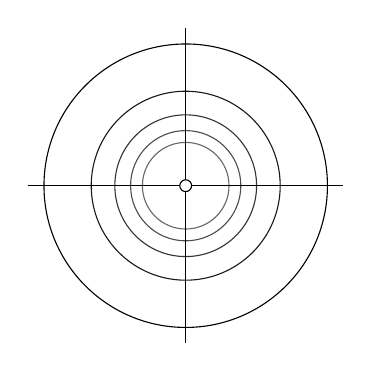
\begin{tikzpicture}
    \draw (-2, 0) -- (2, 0);
    \draw (0, -2) -- (0, 2);

    \draw [fill=white] circle [radius=0.075];
    \draw circle [radius=1.8];
    \draw [opacity=0.9] circle [radius=1.2];
    \draw [opacity=0.8] circle [radius=0.9];
    \draw [opacity=0.7] circle [radius=0.7];
    \draw [opacity=0.6] circle [radius=0.55];
  \end{tikzpicture}
\end{center}
The strategy now is to exploit the fact that $\R^2 \setminus \{0\}$ has circles which cannot be deformed to points.

\subsection{Homotopy}
We have just talked about the notion of ``deforming'' circles to a point. We can think of a circle in $X$ as a map $S^1 \to X$, and we want to ``deform'' this map to a point. This process of deformation is known as \emph{homotopy}. Here we are going to use the interval $[0, 1]\subseteq \R $ a lot, and we will just call it $I$.
\begin{notation}
  \[
    I = [0, 1]\subseteq \R.
  \]
\end{notation}

\begin{defi}[Homotopy]
  Let $f, g: X\to Y$ be maps. A \emph{homotopy} from $f$ to $g$ is a map
  \[
    H: X\times I \to Y
  \]
  such that
  \[
    H(x, 0) = f(x),\quad H(x, 1) = g(x).
  \]
  We think of the interval $I$ as time. For each time $t$, $H(\ph, t)$ defines a map $X\to Y$. So we want to start from $f$, move with time, and eventually reach $g$.

  If such an $H$ exists, we say $f$ is \emph{homotopic} to $g$, and write $f\simeq g$. If we want to make it explicit that the homotopy is $H$, we write $f \simeq_H g$.
\end{defi}
As mentioned at the beginning, by calling $H$ a map, we are requiring it to be continuous.

Sometimes, we don't want a general homotopy. We might want to make sure that when we are deforming from a path $f$ to $g$, the end points of the path don't move. In general, we have
\begin{defi}[Homotopy $\rel$ A]
  We say $f$ is \emph{homotopic to} $g$ $\rel A$, written $f\simeq g\rel A$, if for all $a \in A\subseteq X$, we have
  \[
    H(a, t) = f(a) = g(a).
  \]
\end{defi}
This notion will find itself useful later, but we don't have to pay too much attention to this yet.

Our notation suggests that homotopy is an equivalence relation. Indeed, we have
\begin{prop}
  For spaces $X, Y$, and $A\subseteq X$, the ``homotopic $\rel A$'' relation is an equivalence relation. In particular, when $A = \emptyset$, homotopy is an equivalence relation.
\end{prop}

\begin{proof}\leavevmode
  \begin{enumerate}
    \item Reflexivity: $f \simeq f$ since $H(x, t) = f(x)$ is a homotopy.
    \item Symmetry: if $H(x, t)$ is a homotopy from $f$ to $g$, then $H(x, 1 - t)$ is a homotopy from $g$ to $f$.
    \item Transitivity: Suppose $f, g, h: X\to Y$ and $f\simeq_H g\rel A$, $g\simeq_{H'} h \rel A$. We want to show that $f\simeq h \rel A$. The idea is to ``glue'' the two maps together.

      We know how to continuously deform $f$ to $g$, and from $g$ to $h$. So we just do these one after another.
      We define $H'': X\times I \to Y$ by
      \[
        H''(x, t) =
        \begin{cases}
          H(x, 2t) & 0 \leq t \leq \frac{1}{2}\\
          H'(x, 2t - 1) & \frac{1}{2} \leq t \leq 1
        \end{cases}
      \]
      This is well-defined since $H(x, 1) = g(x) = H'(x, 0)$. This is also continuous by the gluing lemma. It is easy to check that $H''$ is a homotopy $\rel A$.\qedhere
  \end{enumerate}
\end{proof}

We now have a notion of equivalence of maps --- two maps are equivalent if they are homotopic. We can extend the notion of homotopy to spaces as well.

Recall that when we defined homeomorphism, we required that there be some $f, g$ such that $f\circ g = \id$, $g\circ f = \id$. Here, we replace equality by homotopy.
\begin{defi}[Homotopy equivalence]
  A map $f: X\to Y$ is a \emph{homotopy equivalence} if there exists a $g: Y\to X$ such that $f\circ g \simeq \id_Y$ and $g\circ f \simeq \id_X$. We call $g$ a \emph{homotopy inverse} for $f$.

  If a homotopy equivalence $f: X\to Y$ exists, we say that $X$ and $Y$ are homotopy equivalent and write $X\simeq Y$.
\end{defi}
We are soon going to prove that this is indeed an equivalence relation on spaces, but we first look at some examples of homotopy equivalent spaces. Clearly, homeomorphic spaces are homotopy equivalent. However, we will see that we can do much more ``violent'' things to a space and still be homotopy equivalent.
\begin{eg}
  Let $X = S^1$, $Y = \R^2 \setminus \{0\}$. We have a natural inclusion map $i: X\hookrightarrow Y$. To obtain a map $Y \to X$, we can project each point onto the circle.
  \begin{center}
    \begin{tikzpicture}
      \draw (-2, 0) -- (2, 0);
      \draw (0, -2) -- (0, 2);

      \draw [fill=white] circle [radius=0.075];
      \draw circle [radius=1.5];

      \node [circ] at (1.06, 1.06) {};
      \node [circ] at (2, 2) {};
      \node at (1.06, 1.06) [right] {$r(y)$};
      \node at (2, 2) [right] {$y$};
      \draw [dashed] (0.053, 0.053) -- (2, 2);
    \end{tikzpicture}
  \end{center}
  In particular, we define $r: Y\to X$ by
  \[
    r(y) = \frac{y}{\|y\|}.
  \]
  We immediately have $r\circ i = \id_X$. We will now see that $i\circ r \simeq \id_Y$. The composition $i\circ r$ first projects each object into $S^1$, and then includes it back into $\R^2 \setminus \{0\}$. So this is just the projection map. We can define a homotopy $H: Y\times I \to Y$ by
  \[
    H(y, t) = \frac{y}{t + (1 - t)\|y\|}.
  \]
  This is continuous, and $H(\ph, 0) = i\circ r$, $H(\ph, 1) = \id_Y$.
\end{eg}
As we have said, homotopy equivalence can do really ``violent'' things to a space. We started with a 2-dimensional $\R^2\setminus \{0\}$ space, and squashed it into a one-dimensional sphere.

Hence we see that homotopy equivalence doesn't \emph{care} about dimensions. Dimensions seem to be a rather fundamental thing in geometry, and we are discarding it here. So what is left? What does homotopy equivalence preserve?

While $S^1$ and $\R^2 \setminus \{0\}$ seem rather different, they have something in common --- they both have a ``hole''. We will later see that this is what homotopy equivalence preserves.

\begin{eg}
  Let $Y = \R^n$, $X = \{0\} = *$. Let $X\hookrightarrow Y$ be the inclusion map, and $r: Y\to X$ be the unique map that sends everything to $\{0\}$. Again, we have $r\circ i = \id_X$. We can also obtain a homotopy from $i \circ r$ to $\id_Y$ by
  \[
    H(y, t) = ty.
  \]
\end{eg}
Again, from the point of view of homotopy theory, $\R^n$ is just the same as a point! You might think that this is something crazy to do --- we have just given up a lot of structure of topological spaces. However, by giving up these structures, it is easier to focus on what we really want to care about --- holes. For example, it is often much easier to argue about the one-point space $*$ than the whole of $\R^2$! By studying properties that are preserved by homotopy equivalence, and not just homeomorphism, we can simplify our problems by reducing complicated spaces to simpler ones via homotopy equivalence.

In general things homotopy equivalent to a single point are known as \emph{contractible spaces}.
\begin{notation}
  $*$ denotes the one-point space $\{0\}$.
\end{notation}

\begin{defi}[Contractible space]
  If $X\simeq *$, then $X$ is \emph{contractible}.
\end{defi}

We now show that homotopy equivalence of spaces is an equivalence relation. To do this, we first need a lemma.
\begin{lemma}
  Consider the spaces and arrows
  \[
    \begin{tikzcd}
      X \ar[r, bend left, "f_0"] \ar[r, bend right, "f_1"'] & Y \ar[r, bend left, "g_0"] \ar[r, bend right, "g_1"'] & Z
    \end{tikzcd}
  \]
  If $f_0\simeq_H f_1$ and $g_0\simeq_{H'} g_1$, then $g_0\circ f_0 \simeq g_1 \circ f_1$.
\end{lemma}

\begin{proof}
  We will show that $g_0 \circ f_0 \simeq g_0 \circ f_1 \simeq g_1 \circ f_1$. Then we are done since homotopy between maps is an equivalence relation. So we need to write down two homotopies.

  \begin{enumerate}
    \item Consider the following composition:
      \[
        \begin{tikzcd}
          X\times I \ar[r, "H"] & Y \ar[r, "g_0"] & Z
        \end{tikzcd}
      \]
      It is easy to check that this is the first homotopy we need to show $g_0\circ f_0 \simeq g_0 \circ f_1$.
    \item The following composition is a homotopy from $g_0 \circ f_1$ to $g_1 \circ f_1$:
      \[
        \begin{tikzcd}
          X\times I \ar[r, "f_1\times \id_I"] & Y\times I \ar[r, "H'"] & Z
        \end{tikzcd}\qedhere
      \]%\qedhere
  \end{enumerate}
\end{proof}

\begin{prop}
  Homotopy equivalence of spaces is an equivalence relation.
\end{prop}

\begin{proof}
  Symmetry and reflexivity are trivial. To show transitivity, let $f: X \to Y$ and $h: Y \to Z$ be homotopy equivalences, and $g: Y \to X$ and $k: Z \to Y$ be their homotopy inverses. We will show that $h \circ f: X \to Z$ is a homotopy equivalence with homotopy inverse $g \circ k$. We have
  \[
    (h \circ f) \circ (g \circ k) = h \circ (f \circ g) \circ k \simeq h \circ {\id_Y} \circ k = h \circ k \simeq \id_Z.
  \]
  Similarly,
  \[
    (g \circ k) \circ (h \circ f) = g \circ (k \circ h) \circ f \simeq g \circ {\id_Y} \circ f = g \circ f \simeq \id_X.
  \]
  So done.
\end{proof}

\begin{defi}[Retraction]
  Let $A\subseteq X$ be a subspace. A \emph{retraction} $r: X\to A$ is a map such that $r\circ i = \id_A$, where $i: A\hookrightarrow X$ is the inclusion. If such an $r$ exists, we call $A$ a \emph{retract} of $X$.
\end{defi}
This map sends everything in $X$ to $A$ without moving things in $A$. Roughly speaking, if such a retraction exists, then $A$ is no more complicated than $X$.

\begin{defi}[Deformation retraction]
  The retraction $r$ is a \emph{deformation retraction} if $i\circ r \simeq \id_X$. A deformation retraction is \emph{strong} if we require this homotopy to be a homotopy rel $A$.
\end{defi}
Roughly, this says that $A$ is as complicated as $X$.

\begin{eg}
  Take $X$ any space, and $A = \{x\}\subseteq X$. Then the constant map $r: X\to A$ is a retraction. If $X$ is contractible, then $A$ is a deformation retract of $X$.
\end{eg}

\subsection{Paths}
\begin{defi}[Path]
  A \emph{path} in a space $X$ is a map $\gamma: I\to X$. If $\gamma(0) = x_0$ and $\gamma(1) = x_1$, we say $\gamma$ is a path from $x_0$ to $x_1$, and write $\gamma: x_0 \rightsquigarrow x_1$.

  If $\gamma(0) = \gamma(1)$, then $\gamma$ is called a \emph{loop} (based at $x_0$).
  \begin{center}
    \begin{tikzpicture}
      \draw plot [smooth cycle] coordinates {(-1.2, -0.7) (0, -0.7) (0.7, -1) (1.3, -0.9) (1.4, 0.6) (0.3, 0.9) (-1.7, 0.8)};

      \node [circ] at (-1, 0.2) {};
      \node [above] at (-1, 0.2) {$x_0$};
      \node [circ] at (0.8, 0.1) {};
      \node [above] at (0.8, 0.1) {$x_1$};
      \draw plot [smooth] coordinates {(-1, 0.2) (-0.3, 0) (0.1, 0.3) (0.8, 0.1)};
    \end{tikzpicture}
  \end{center}
\end{defi}
Note that this map does not have to be injective. It can be self-intersecting or do all sorts of weird stuff.

Recall that the basic idea of algebraic topology is to assign to each space $X$ an (algebraic) object, which is (hopefully) easier to deal with. In homotopy theory, we do so using the idea of paths.

To do so, we need to be able to perform operations on paths.
\begin{defi}[Concatenation of paths]
  If we have two paths $\gamma_1$ from $x_0$ to $x_1$; and $\gamma_2$ from $x_1$ to $x_2$, we define the \emph{concatenation} to be
  \[
    (\gamma_1\cdot \gamma_2)(t) =
    \begin{cases}
      \gamma_1(2t) & 0 \leq t \leq \frac{1}{2}\\
      \gamma_2(2t - 1) & \frac{1}{2} \leq t \leq 1.
    \end{cases}
  \]
  This is continuous by the gluing lemma.
\end{defi}
Note that we concatenate left to right, but function composition goes from right to left.
\begin{center}
  \begin{tikzpicture}
    \draw plot [smooth cycle] coordinates {(-2.4, -0.7) (0, -0.7) (1.4, -1) (2.6, -0.9) (2.8, 0.6) (0.6, 1.9) (-3.4, 0.8)};

    \node [circ] at (-2, 0.2) {};
    \node [above] at (-2, 0.2) {$x_0$};
    \node [circ] at (-0.2, 0.1) {};
    \node [above] at (-0.2, 0.1) {$x_1$};
    \node [circ] at (2, 0.5) {};
    \node [above] at (2, 0.5) {$x_2$};
    \draw plot [smooth] coordinates {(-2, 0.2) (-1.3, 0) (-0.9, 0.3) (-0.2, 0.1) (1, 0.6) (2, 0.5)};
  \end{tikzpicture}
\end{center}
\begin{defi}[Inverse of path]
  The \emph{inverse} of a path $\gamma: I \to X$ is defined by
  \[
    \gamma^{-1}(t) = \gamma(1 - t).
  \]
  This is exactly the same path but going in the opposite direction.
\end{defi}

What else do we need? We need an identity.
\begin{defi}[Constant path]
  The \emph{constant path} at a point $x\in X$ is given by $c_x(t) = x$.
\end{defi}

We haven't actually got a good algebraic system. We have $\gamma$ and $\gamma^{-1}$, but when we compose them, we get a path from $x_1$ to $x_2$ and back, and not the identity. Also, we are not able to combine arbitrary paths in a space.

Before we make these into proper algebraic operations, we will talk about something slightly different. We can view this as a first attempt at associating things to topological spaces.

\begin{defi}[Path components]
  We can define a relation on $X$: $x_1 \sim x_2$ if there exists a path from $x_1$ to $x_2$. By the concatenation, inverse and constant paths, $\sim$ is an equivalence relation. The equivalence classes $[x]$ are called \emph{path components}. We denote the quotient $X/{\sim}$ by $\pi_0(X)$.
\end{defi}
\begin{center}
  \begin{tikzpicture}[scale=0.5]
    \draw [fill=mblue, opacity=0.5] circle [radius = 1];
    \draw (3, 2.5) [fill=mblue, opacity=0.5] circle [radius = 1.3];
    \draw (6, 1) [fill=mblue, opacity=0.5] circle [radius = 1.2];
  \end{tikzpicture}
\end{center}
In the above space, we have three path components.

This isn't really a very useful definition, since most spaces we care about are path-connected, i.e.\ only have one path component. However, this is a first step at associating \emph{something} to spaces. We can view this as a ``toy model'' for the more useful definitions we will later have.

One important property of this $\pi_0$ is that not only does it associate a set to each topological space, but also associates a function between the corresponding sets to each continuous map.
\begin{prop}
  For any map $f: X\to Y$, there is a well-defined function
  \[
    \pi_0(f): \pi_0(X) \to \pi_0(Y),
  \]
  defined by
  \[
    \pi_0(f)([x]) = [f(x)].
  \]
  Furthermore,
  \begin{enumerate}
    \item If $f\simeq g$, then $\pi_0(f) = \pi_0(g)$.
    \item For any maps $\begin{tikzcd} A \ar[r, "h"] & B\ar[r, "k"] & C\end{tikzcd}$, we have $\pi_0(k\circ h) = \pi_0(k)\circ \pi_0 (h)$.
    \item $\pi_0(\id_X) = \id_{\pi_0(X)}$
  \end{enumerate}
\end{prop}

\begin{proof}
  To show this is well-defined, suppose $[x] = [y]$. Then let $\gamma: I \to X$ be a path from $x$ to $y$. Then $f \circ \gamma$ is a path from $f(x)$ to $f(y)$. So $[f(x)] = [f(y)]$.
  \begin{enumerate}
    \item If $f \simeq g$, let $H: X \times I \to Y$ be a homotopy from $f$ to $g$. Let $x \in X$. Then $H(x, \ph)$ is a path from $f(x)$ to $g(x)$. So $[f(x)] = [g(x)]$, i.e.\ $\pi_0(f)([x]) = \pi_0(g)([x])$. So $\pi_0(f) = \pi_0(g)$.
    \item $\pi_0(k \circ h)([x]) = \pi_0(k) \circ \pi_0(h)([x]) = [k(h(x))]$.
    \item $\pi_0(\id_X)([x]) = [\id_X(x)] = [x]$. So $\pi_0(\id_X) = \id_{\pi_0(X)}$.\qedhere
  \end{enumerate}
\end{proof}

\begin{cor}
  If $f: X\to Y$ is a homotopy equivalence, then $\pi_0(f)$ is a bijection.
\end{cor}

\begin{eg}
  The two point space $X = \{-1, 1\}$ is not contractible, because $|\pi_0(X)| = 2$, but $|\pi_0(*)| = 1$.
\end{eg}
This is a rather silly example, since we can easily prove it directly. However, this is an example to show how we can use this machinery to prove topological results.

Now let's return to our operations on paths, and try to make them algebraic.

\begin{defi}[Homotopy of paths]
  Paths $\gamma, \gamma': I\to X$ are \emph{homotopic as paths} if they are homotopic rel $\{0, 1\}\subseteq I$, i.e.\ the end points are fixed. We write $\gamma\simeq \gamma'$.
\end{defi}
\begin{center}
  \begin{tikzpicture}
    \draw plot [smooth cycle] coordinates {(-1.2, -0.7) (0, -0.7) (0.7, -1) (1.3, -0.9) (1.4, 0.6) (0.3, 1.2) (-1.7, 0.8)};

    \node [circ] at (-1, 0.2) {};
    \node [left] at (-1, 0.2) {$x_0$};
    \node [circ] at (0.8, 0.1) {};
    \node [right] at (0.8, 0.1) {$x_1$};
    \draw [semithick, mred] plot [smooth] coordinates {(-1, 0.2) (-0.5, 0.6) (0.1, 0.8) (0.8, 0.1)};
    \draw [semithick, mred!50!mblue] plot [smooth] coordinates {(-1, 0.2) (-0.3, 0) (0.1, 0.3) (0.8, 0.1)};
    \draw [semithick, mblue] plot [smooth] coordinates {(-1, 0.2) (-0.3, -0.5) (0.4, -0.5) (0.8, 0.1)};
  \end{tikzpicture}
\end{center}
Note that we would necessarily want to fix the two end points. Otherwise, if we allow end points to move, we can shrink any path into a constant path, and our definition of homotopy would be rather silly.

This homotopy works well with our previous operations on paths.
\begin{prop}
  Let $\gamma_1, \gamma_2: I \to X$ be paths, $\gamma_1(1) = \gamma_2(0)$. Then if $\gamma_1\simeq \gamma_1'$ and $\gamma_2 \simeq \gamma_2'$, then $\gamma_1 \cdot \gamma_2 \simeq \gamma_1' \cdot \gamma_2'$.
\end{prop}
\begin{center}
  \begin{tikzpicture}
    \draw plot [smooth cycle] coordinates {(-2.4, -0.7) (0, -0.7) (1.4, -1) (2.6, -0.9) (2.8, 0.6) (0.6, 1.9) (-3.4, 0.8)};

    \node [circ] at (-2, 0.2) {};
    \node [anchor = south east] at (-2, 0.2) {$x_0$};
    \node [circ] at (-0.2, 0.1) {};
    \node [above] at (-0.2, 0.1) {$x_1$};
    \node [circ] at (2, 0.5) {};
    \node [above] at (2, 0.5) {$x_2$};
    \draw [semithick, mred] (-2, 0.2) parabola bend (-1.1, -0.3) (-0.2, 0.1);
    \draw [semithick, mred] (-0.2, 0.1) parabola bend (1, -0.5) (2, 0.5);

    \draw [semithick, mblue] (-2, 0.2) parabola bend (-1.3, 0.7) (-0.2, 0.1);
    \draw [semithick, mblue] (-0.2, 0.1) parabola bend (1.3, 0.7) (2, 0.5);

    \node [mred, below] at (-1.1, -0.3) {$\gamma_1$};
    \node [mred, below] at (1, -0.5) {$\gamma_2$};

    \node [mblue, above] at (-1.3, 0.7) {$\gamma_1'$};
    \node [mblue, above] at (1, 0.7) {$\gamma_2'$};
  \end{tikzpicture}
\end{center}

\begin{proof}
  Suppose that $\gamma_1 \simeq_{H_1}\gamma_1'$ and $\gamma_2\simeq_{H_2}\gamma_2'$. Then we have the diagram
  \begin{center}
    \begin{tikzpicture}
      \draw (0, 0) rectangle (2, 2);
      \draw (2, 0) rectangle (4, 2);
      \node at (1, 0) [below] {\small$\gamma_1$};
      \node at (3, 0) [below] {\small$\gamma_2$};
      \node at (1, 2) [above] {\small$\gamma_1'$};
      \node at (3, 2) [above] {\small$\gamma_2'$};
      \node at (0, 1) [left] {\small$x_0$};
      \node at (2, 1) [left] {\small$x_1$};
      \node at (4, 1) [right] {\small$x_2$};

      \node at (1, 1) {\large $H_1$};
      \node at (3, 1) {\large $H_2$};
    \end{tikzpicture}
  \end{center}
  We can thus construct a homotopy by
  \[
    H(s, t) =
    \begin{cases}
      H_1(s, 2t) & 0 \leq t \leq \frac{1}{2}\\
      H_2(s, 2t - 1) & \frac{1}{2} \leq t \leq 1
    \end{cases}.\qedhere
  \]
\end{proof}

To solve all our previous problems about operations on paths not behaving well, we can look at paths \emph{up to homotopy}.
\begin{prop}
  Let $\gamma_0: x_0 \leadsto x_1, \gamma_1: x_1 \leadsto x_2, \gamma_2: x_2 \leadsto x_3$ be paths. Then
  \begin{enumerate}
    \item $(\gamma_0 \cdot \gamma_1)\cdot \gamma_2 \simeq \gamma_0 \cdot (\gamma_1\cdot \gamma_2)$
    \item $\gamma_0 \cdot c_{x_1}\simeq \gamma_0 \simeq c_{x_0}\cdot \gamma_0$.
    \item $\gamma_0 \cdot \gamma_0^{-1}\simeq c_{x_0}$ and $\gamma_0^{-1}\cdot \gamma_0 \simeq c_{x_1}$.
  \end{enumerate}
\end{prop}

\begin{proof}\leavevmode
  \begin{enumerate}
    \item Consider the following diagram:
      \begin{center}
        \begin{tikzpicture}[scale=0.75]
          \draw rectangle (4, 4);

          \node at (0, 2) [left] {\small$x_0$};
          \node at (4, 2) [right] {\small$x_3$};

          \node [circ] at (1, 0) {};
          \node [circ] at (2, 0) {};
          \node [circ] at (2, 4) {};
          \node [circ] at (3, 4) {};

          \node [below] at (0.5, 0) {\small$\gamma_0$};
          \node [below] at (1.5, 0) {\small$\gamma_1$};
          \node [below] at (3, 0) {\small$\gamma_2$};

          \node [above] at (1, 4) {\small$\gamma_0$};
          \node [above] at (2.5, 4) {\small$\gamma_1$};
          \node [above] at (3.5, 4) {\small$\gamma_2$};

          \draw (1, 0) -- (2, 4) node [pos=0.5, left] {\small$x_1$};
          \draw (2, 0) -- (3, 4) node [pos=0.5, left] {\small$x_2$};
        \end{tikzpicture}
      \end{center}
    \item Consider the following diagram:
      \begin{center}
        \begin{tikzpicture}[scale=0.75]
          \draw rectangle (4, 4);
          \node [circ] at (2, 0) {};
          \node at (1, 0) [below] {\small$\gamma_0$};
          \node at (3, 0) [below] {\small$c_{x_1}$};
          \node at (2, 4) [above] {\small$\gamma_0$};
          \node at (0, 2) [left] {\small$x_0$};
          \node at (4, 2) [right] {\small$x_1$};

          \draw (2, 0) -- (4, 4) node [pos=0.5, left] {\small$x_1$};
        \end{tikzpicture}
      \end{center}
    \item Consider the following diagram:
      \begin{center}
        \begin{tikzpicture}[scale=0.75]
          \draw rectangle (4, 4);
          \node [circ] at (2, 0) {};
          \node at (1, 0) [below] {\small$\gamma_0$};
          \node at (3, 0) [below] {\small$\gamma_0^{-1}$};
          \node at (2, 4) [above] {\small$c_{x_0}$};
          \node at (0, 2) [left] {\small$x_0$};
          \node at (4, 2) [right] {\small$x_0$};

          \draw (0, 4) -- (2, 0) -- (4, 4);
        \end{tikzpicture}
      \end{center}
  \end{enumerate}
  Turning these into proper proofs is left as an exercise for the reader.
\end{proof}

\subsection{The fundamental group}
The idea is to take spaces and turn them into groups. We want to try to do this using paths. We've seen that if we want to do this, we should not work directly with paths, but paths up to homotopy. According to our proposition, this operation satisfies associativity, inverses and identity. The last issue we have to resolve is that we can't actually put two paths together unless they have the same start and end points.

The idea is to fix one of the points $x_0$ in our space, and only think about loops that start and end at $x_0$. So we can always join two paths together.

This tells us that we aren't going to just think about spaces, but spaces \emph{with basepoints}. We've now got everything we need.

\begin{defi}[Fundamental group]
  Let $X$ be a space and $x_0 \in X$. The \emph{fundamental group} of $X$ (based at $x_0$), denoted $\pi_1(X, x_0)$, is the set of homotopy classes of loops in $X$ based at $x_0$ (i.e.\ $\gamma(0) = \gamma(1) = x_0$). The group operations are defined as follows:

  We define an operation by $[\gamma_0][\gamma_1] = [\gamma_0\cdot \gamma_1]$; inverses by $[\gamma]^{-1} = [\gamma^{-1}]$; and the identity as the constant path $e = [c_{x_0}]$.
\end{defi}
Often, when we write the homotopy classes of paths $[\gamma]$, we just get lazy and write $\gamma$.

\begin{thm}
  The fundamental group is a group.
\end{thm}

\begin{proof}
  Immediate from our previous lemmas.
\end{proof}

Often, in mathematics, after defining a term, we give lots of examples of it. Unfortunately, it is rather difficult to prove that a space has a non-trivial fundamental group, until we have developed some relevant machinery. Hence we will have to wait for a while before we have some concrete examples. Instead, we will look at some properties of the fundamental group first.

\begin{defi}[Based space]
  A \emph{based space} is a pair $(X, x_0)$ of a space $X$ and a point $x_0\in X$, the \emph{basepoint}. A \emph{map of based spaces}
  \[
    f: (X, x_0) \to (Y, y_0)
  \]
  is a continuous map $f: X\to Y$ such that $f(x_0) = y_0$. A \emph{based homotopy} is a homotopy rel $\{x_0\}$.
\end{defi}

Recall that for $\pi_0$, to every map $f: X\to Y$, we can associate a function $\pi_0(f): \pi_0(X) \to \pi_0(Y)$. We can do the same for $\pi_1$.
\begin{prop}
  To a based map
  \[
    f: (X, x_0) \to (Y, y_0),
  \]
  there is an associated function
  \[
    f_* = \pi_1(f): \pi_1(X, x_0) \to \pi_1(Y, y_0),
  \]
  defined by $[\gamma] \mapsto [f\circ \gamma]$. Moreover, it satisfies
  \begin{enumerate}
    \item $\pi_1(f)$ is a homomorphism of groups.
    \item If $f \simeq f'$, then $\pi_1(f) = \pi_1(f')$.
    \item For any maps $\begin{tikzcd} (A, a) \ar[r, "h"] & (B, b) \ar[r, "k"] & (C, c) \end{tikzcd}$, we have $\pi_1(k\circ h) = \pi_1(k)\circ \pi_1 (h)$.
    \item $\pi_1(\id_X) = \id_{\pi_1(X, x_0)}$
  \end{enumerate}
\end{prop}

\begin{proof}
  Exercise. % fill in
\end{proof}
In category-theoretic language, we say that $\pi_1$ is a \emph{functor}.

So far so good. However, to define the fundamental group, we had to make a compromise and pick a basepoint. But we just care about the space. We don't want a basepoint! Hence, we should look carefully at what happens when we change the basepoint, and see if we can live without it.

The first observation is that $\pi_1(X, x_0)$ only ``sees'' the path component of $x_0$, since all loops based at $x_0$ can only live inside the path component of $x_0$. Hence, the first importance of picking a basepoint is picking a path component.

For all practical purposes, we just assume that $X$ is path connected, since if we weren't, the fundamental group just describes a particular path component of the original space.

Now we want to compare fundamental groups with different basepoints. Suppose we have two basepoints $x_0$ and $x_1$. Suppose we have a loop $\gamma$ at $x_0$. How can we turn this into a loop based at $x_1$? This is easy. We first pick a path $u: x_0 \leadsto x_1$. Then we can produce a new loop at $x_1$ by going along $u^{-1}$ to $x_0$, take the path $\gamma$, and then return to $x_0$ by $u$, i.e.\ consider $u^{-1}\cdot \gamma\cdot u$.
\begin{center}
  \begin{tikzpicture}
    \draw plot [smooth cycle] coordinates {(-2.4, -0.7) (0, -0.7) (1.4, -1) (2.6, -0.9) (2.8, 0.6) (0.6, 1.9) (-3.4, 0.8)};

    \node [circ] at (-2, 0.2) {};
    \node [anchor = south west] at (-2, 0.2) {$x_0$};
    \node [circ] at (1.5, 0.1) {};
    \node [above] at (1.5, 0.1) {$x_1$};

    \draw [->-=0.5] (-2.4, 0.2) circle [radius = 0.4];
    \draw [->-=0.5] (-2, 0.2) parabola bend (-0.25, 0) (1.5, 0.1) node [pos=0.5, below] {$u$};
    \draw [mred, ->-=0.3, ->-=0.7] (1.5, 0.1) -- (1.5, 0.2) parabola bend (-0.25, 0.1) (-2, 0.3) arc (14:346:0.4123) parabola bend (-0.25, -0.1) (1.5, 0) -- (1.5, 0.1);
  \end{tikzpicture}
\end{center}

\begin{prop}
  A path $u: x_0 \leadsto x_1$ induces a group \emph{isomorphism}
  \[
    u_\#: \pi_1(X, x_0) \to \pi_1(X, x_1)
  \]
  by
  \[
    [\gamma] \mapsto [u^{-1}\cdot \gamma \cdot u].
  \]
  This satisfies
  \begin{enumerate}
    \item If $u\simeq u'$, then $u_\# = u'_\#$.
    \item $(c_{x_0})_\# = \id_{\pi_1(X, x_0)}$
    \item If $v: x_1 \leadsto x_2$. Then $(u\cdot v)_\# = v_\# \circ u_\#$.
    \item If $f: X\to Y$ with $f(x_0) = y_0$, $f(x_1) = y_1$, then
      \[
        (f\circ u)_\# \circ f_* = f_* \circ u_\#: \pi_1(X, x_0) \to \pi_1(Y, y_1).
      \]
      A nicer way of writing this is
      \[
        \begin{tikzcd}[row sep=large]
          \pi_1(X, x_0) \ar[r, "f_*"] \ar[d, "u_\#"] & \pi_1(Y, y_0)\ar [d, "(f\circ u)_\#"]\\
          \pi_1(X, x_1) \ar[r, "f_*"] & \pi_1(Y, y_1)
        \end{tikzcd}
      \]
      The property says that the composition is the same no matter which way we go from $\pi_1(X, x_0)$ to $\pi_1(Y, y_1)$. We say that the square is a \emph{commutative diagram}. These diagrams will appear all of the time in this course.
    \item If $x_1 = x_0$, then $u_\#$ is an automorphism of $\pi_1(X, x_0)$ given by conjugation by $u$.
  \end{enumerate}
\end{prop}
It is important (yet difficult) to get the order of concatenation and composition right. Path concatenation is from left to right, while function composition is from right to left.

\begin{proof}
  Yet another exercise. Note that $(u^{-1})_\# = (u_\#)^{-1}$, which is why we have an isomorphism. %fill in
\end{proof}
The main takeaway is that if $x_0$ and $x_1$ are in the same path component, then
\[
  \pi_1(X, x_0) \cong \pi_1(X, x_1).
\]
So the basepoint isn't really too important. However, we have to be careful. While the two groups are isomorphic, the actual isomorphism depends on \emph{which} path $u: x_0 \leadsto x_1$ we pick. So there is no natural isomorphism between the two groups. In particular, we cannot say ``let $\alpha \in \pi_1(X, x_0)$. Now let $\alpha'$ be the corresponding element in $\pi_1(X, x_1)$''.

We can also see that if $(X, x_0)$ and $(Y, y_0)$ are based homotopy equivalent, then $\pi_1(X, x_0)\cong \pi_1(Y, y_0)$. Indeed, if they are homotopy equivalent, then there are some $f: X \to Y$, $g: Y \to X$ such that
\[
  f\circ g \simeq \id_Y,\quad g\circ f \simeq \id_X.
\]
So
\[
  f_*\circ g_* = \id_{\pi_1(Y, y_0)},\quad g_*\circ f_* = \id_{\pi_1(X, x_0)},
\]
and $f_*$ and $g_*$ are the isomorphisms we need.

However, can we do this with non-based homotopies? Suppose we have a space $X$, and a space $Y$, and functions $f, g: X \to Y$, with a homotopy $H: X\times I \to Y$ from $f$ to $g$. If this were a based homotopy, we know
\[
  f_* = g_*: \pi_1(X, x_0) \to \pi_1(Y, f(x_0)).
\]
Now we don't insist that this homotopy fixes $x_0$, and we could have $f(x_0) \not= g(x_0)$. How can we relate $f_*: \pi_1(X, x_0) \to \pi_1(Y, f(x_0))$ and $g_*: \pi_1(X, x_0) \to \pi_1(Y, g(x_0))$?

First of all, we need to relate the groups $\pi_1(Y, f(x_0))$ and $\pi_1(Y, g(x_0))$. To do so, we need to find a path from $f(x_0)$ to $g(x_0)$. To produce this, we can use the homotopy $H$. We let $u: f(x_0) \leadsto g(x_0)$ with $u = H(x_0, \ph)$. Now we have three maps $f_*, g_*$ and $u_\#$. Fortunately, these do fit together well.
\begin{center}
  \begin{tikzpicture}
    \draw plot [smooth cycle] coordinates {(-3.7, -1.2) (-3.7, 0) (-4, 0.7) (-3.9, 1.3) (-2.4, 1.4) (-1.8, 0.3) (-2.2, -1.7)};
    \draw plot [smooth cycle] coordinates {(1.3, -1.2) (1.3, 0) (0.7, 0.7) (0.6, 1.3) (2.6, 1.4) (3, 0.3) (2.8, -1.7)};

    \node [circ] at (-3, 0) {};
    \node [below] at (-3, 0) {$x_0$};
    \node [above] at (-3, 1.6) {$X$};

    \node [above] at (1.8, 1.6) {$Y$};

    \node [circ] at (1.8, 0.8) {};
    \node [below] at (1.8, 0.8) {$f(x_0)$};

    \node [circ] at (2, -0.8) {};
    \node [below] at (2, -0.8) {$g(x_0)$};

    \draw [->] (-1.6, 1) parabola bend (-0.7, 1.3) (0.2, 1.2);
    \node [above] at (-0.7, 1.3) {$f$};

    \draw [->] (-1.6, -1) parabola bend (-0.3, -1.3) (1, -1.1);
    \node [below] at (-0.3, -1.3) {$g$};
  \end{tikzpicture}
\end{center}

\begin{lemma}
  The following diagram commutes:
  \[
    \begin{tikzcd}
      & \pi_1(Y, f(x_0)) \ar[dd, "u_\#"]\\
      \pi_1(X, x_0) \ar[ru, "f_*"] \ar [rd, "g_*"']& \\
      & \pi_1(Y, g(x_0))
    \end{tikzcd}
  \]
  In algebra, we say
  \[
    g_* = u_\# \circ f_*.
  \]
\end{lemma}

\begin{proof}
  Suppose we have a loop $\gamma: I\to X$ based at $x_0$.

  We need to check that
  \[
    g_*([\gamma]) = u_\#\circ f_*([\gamma]).
  \]
  In other words, we want to show that
  \[
    g\circ \gamma \simeq u^{-1}\cdot (f\circ \gamma)\cdot u.
  \]
  To prove this result, we want to build a homotopy.

  Consider the composition:
  \[
    F:
    \begin{tikzcd}
      I\times I \ar[r, "\gamma\times \id_I"] & X\times I \ar[r, "H"] & Y.
    \end{tikzcd}
  \]
  Our plan is to exhibit two homotopic paths $\ell^+$ and $\ell^-$ in $I\times I$ such that
  \[
    F\circ \ell^+ = g \circ \gamma,\quad F\circ \ell^- = u^{-1}\cdot (f\circ \gamma) \cdot u.
  \]
  This is in general a good strategy --- $X$ is a complicated and horrible space we don't understand. So to construct a homotopy, we make ourselves work in a much nicer space $I\times I$.

  Our $\ell^+$ and $\ell^-$ are defined in a rather simple way.
  \begin{center}
    \begin{tikzpicture}[scale=0.75]
      \node at (2, 5) {$I\times I$};
      \draw [mgreen, ->-=0.5] (0, 4) -- (0, 0);
      \draw [mgreen, ->-=0.5] (0, 0) -- (4, 0) node [pos=0.5, below] {$\ell^-$};
      \draw [mgreen, ->-=0.5] (4, 0) -- (4, 4);

      \draw [mred, ->-=0.5] (0, 4) -- (4, 4) node [pos=0.5, above] {$\ell^+$};

      \draw [->] (4.5, 2) -- (6.5, 2) node [pos=0.5, above] {$F$};
      \begin{scope}[shift={(7, 0)}]
      \node at (2, 5) {$Y$};
        \draw [->-=0.5] (0, 4) -- (0, 0) node [pos=0.5, right] {$u^{-1}$};
        \draw [->-=0.5] (0, 0) -- (4, 0) node [pos=0.5, below] {$f$};
        \draw [->-=0.5] (4, 0) -- (4, 4) node [pos=0.5, right] {$u$};

        \draw [->-=0.5] (0, 4) -- (4, 4) node [pos=0.5, above] {$g$};
      \end{scope}

    \end{tikzpicture}
  \end{center}
  More precisely, $\ell^+$ is the path $s\mapsto (s, 1)$, and $\ell^-$ is the concatenation of the paths $s\mapsto (0, 1- s)$, $s \mapsto (s, 0)$ and $s\mapsto (1, s)$.

  Note that $\ell^+$ and $\ell^-$ are homotopic as paths. If this is not obvious, we can manually check the homotopy
  \[
    L(s, t) = t\ell^+(s) + (1 - t)\ell^- (s).
  \]
  This works because $I\times I$ is convex. Hence $F\circ \ell^+\simeq_{F\circ L} F\circ \ell^-$ as paths.

  Now we check that the compositions $F\circ \ell^{\pm}$ are indeed what we want. We have
  \[
    F\circ \ell^+ (s) = H(\gamma(s), 1) = g\circ \gamma (s).
  \]
  Similarly, we can show that
  \[
    F\circ \ell^-(s) = u^{-1}\cdot (f\circ \gamma)\cdot u (s).
  \]
  So done.
\end{proof}
It is worth looking at this proof hard and truly understand what is going on, since this is a really good example of how we can construct interesting homotopies.

With this lemma, we can show that fundamental groups really respect homotopies.

\begin{thm}
  If $f: X\to Y$ is a homotopy equivalence, and $x_0 \in X$, then the induced map
  \[
    f_*: \pi_1(X, x_0) \to \pi_1(Y, f(x_0)).
  \]
  is an isomorphism.
\end{thm}
While this seems rather obvious, it is actually non-trivial if we want to do it from scratch. While we are given a homotopy equivalence, we are given no guarantee that the homotopy respects our basepoints. So this proof involves some real work.

\begin{proof}
  Let $g: Y\to X$ be a homotopy inverse. So $f\circ g\simeq_H \id_Y$ and $g\circ f\simeq_{H'} \id_X$.
  \begin{center}
    \begin{tikzpicture}
      \draw plot [smooth cycle] coordinates {(-3.7, -1.2) (-3.7, 0) (-4, 0.7) (-3.9, 1.3) (-2.4, 1.4) (-1.8, 0.3) (-2.2, -1.7)};
      \draw plot [smooth cycle] coordinates {(1.3, -1.2) (1.3, 0) (0.7, 0.7) (0.6, 1.3) (2.6, 1.4) (3, 0.3) (2.8, -1.7)};

      \node [circ] at (-3, 0.7) {};
      \node [above] at (-3, 0.7) {$x_0$};
      \node [above] at (-3, 1.6) {$X$};

      \node [above] at (1.8, 1.6) {$Y$};

      \node [circ] at (1.8, 0.8) {};
      \node [below] at (1.8, 0.8) {$f(x_0)$};

      \node [circ] at (-3, -0.8) {};
      \node [below] at (-3, -0.8) {$g\circ f(x_0)$};

      \draw [decoration={snake}, decorate] (-3, 0.7) -- (-3, -0.8) node [right, pos=0.5] {$u'$};

      \draw [->] (-1.6, 1) parabola bend (-0.7, 1.3) (0.2, 1.2);
      \node [above] at (-0.7, 1.3) {$f$};

      \draw [->] (1, -1.1) parabola bend (-0.3, -1.3) (-1.6, -1);
      \node [below] at (-0.3, -1.3) {$g$};
    \end{tikzpicture}
  \end{center}
  We have no guarantee that $g\circ f(x_0) = x_0$, but we know that our homotopy $H'$ gives us $u' = H'(x_0, \ph): x_0 \leadsto g\circ f(x_0)$.

  Applying our previous lemma with $\id_X$ for ``$f$'' and $g \circ f$ for ``$g$'', we get
  \[
    u'_\# \circ (\id_X)_* = (g\circ f)_*
  \]
  Using the properties of the $_*$ operation, we get that
  \[
    g_*\circ f_* = u'_\#.
  \]
  However, we know that $u'_\#$ is an isomorphism. So $f_*$ is injective and $g_*$ is surjective.

  Doing it the other way round with $f\circ g$ instead of $g\circ f$, we know that $g_*$ is injective and $f_*$ is surjective. So both of them are isomorphisms.
\end{proof}
With this theorem, we can finally be sure that the fundamental group is a property of the space, without regards to the basepoint (assuming path connectedness), and is preserved by arbitrary homotopies.

We now use the fundamental group to define several simple notions.
\begin{defi}[Simply connected space]
  A space $X$ is \emph{simply connected} if it is path connected \emph{and} $\pi_1(X, x_0) \cong 1$ for some (any) choice of $x_0 \in X$.
\end{defi}

\begin{eg}
  Clearly, a point $*$ is simply connected since there is only one path on $*$ (the constant path). Hence, any contractible space is simply connected since it is homotopic to $*$. For example, $\R^n$ is simply connected for all $n$.
\end{eg}

There is a useful characterization of simply connected spaces:
\begin{lemma}
  A path-connected space $X$ is simply connected if and only if for any $x_0, x_1\in X$, there exists a unique homotopy class of paths $x_0 \leadsto x_1$.
\end{lemma}

\begin{proof}
  Suppose $X$ is simply connected, and let $u, v: x_0 \leadsto x_1$ be paths. Now note that $u \cdot v^{-1}$ is a loop based at $x_0$, it is homotopic to the constant path, and $v^{-1} \cdot v$ is trivially homotopic to the constant path. So we have
  \[
    u \simeq u \cdot v^{-1} \cdot v \simeq v.
  \]
  On the other hand, suppose there is a unique homotopy class of paths $x_0 \leadsto x_1$ for all $x_0, x_1 \in X$. Then in particular there is a unique homotopy class of loops based at $x_0$. So $\pi_1(X, x_0)$ is trivial.
\end{proof}

\section{Covering spaces}
We can ask ourselves a question --- what are groups? We can write down a definition in terms of operations and axioms, but this is not what groups \emph{are}. Groups were created to represent \emph{symmetries} of objects. In particular, a group should be \emph{acting} on something. If not, something wrong is probably going on.

We have created the fundamental group. So what do they act on? Can we find something on which these fundamental groups act on?

An answer to this would also be helpful in more practical terms. So far we have not exhibited a non-trivial fundamental group. This would be easy if we can make the group act on something --- if the group acts non-trivially on our thing, then clearly the group cannot be trivial.

These things we act on are \emph{covering spaces}.

\subsection{Covering space}
Intuitively, a \emph{covering space} of $X$ is a pair $(\tilde{X}, p: \tilde{X} \to X)$, such that if we take any $x_0 \in X$, there is some neighbourhood $U$ of $x_0$ such that the pre-image of the neighbourhood is ``many copies'' of $U$.
\begin{center}
  \begin{tikzpicture}
    \draw plot [smooth cycle] coordinates {(-1.2, -0.7) (0, -0.7) (0.7, -1) (1.3, -0.9) (1.4, 0.4) (0.3, 1) (-1.7, 0.6)};

    \draw [fill=morange] ellipse (0.6 and 0.3);
    \node at (0.6, 0.3) [anchor = south east] {$U$};

    \draw [densely dashed] (0, 1.5) -- (0, 0);
    \foreach \y in {1.5, 2, 2.5, 3} {
      \node [circ] at (0, \y) {};
      \pgfmathsetmacro\c{100 - \y * 30};
      \draw [densely dashed] (0, \y) -- (0, \y - 0.5);
      \draw [fill=morange!\c!yellow] (0, \y) ellipse (0.6 and 0.3);
      \node [circ] at (0, \y) {};
    }
    \node [circ] at (0, 0) {};
    \node [left] at (0, 0) {$x_0$};

    \draw [->] (2.3, 2.5) node [above] {$\tilde{X}$}-- +(0, -2.3) node [pos=0.5, right] {$p$} node [below] {$X$};
  \end{tikzpicture}
\end{center}

\begin{defi}[Covering space]
  A \emph{covering space} of $X$ is a pair $(\tilde{X}, p: \tilde{X} \to X)$, such that each $x\in X$ has a neighbourhood $U$ which is \emph{evenly covered}.
\end{defi}
Whether we require $p$ to be surjective is a matter of taste. However, it will not matter if $X$ is path-connected, which is the case we really care about.

\begin{defi}[Evenly covered]
  $U \subseteq X$ is \emph{evenly covered} by $p: \tilde{X} \to X$ if
  \[
    p^{-1}(U) \cong \coprod_{\alpha \in \Lambda}V_\alpha,
  \]
  where $p|_{V_\alpha}: V_\alpha \to U$ is a homeomorphism, and each of the $V_\alpha \subseteq \tilde{X}$ is open.
\end{defi}

\begin{eg}
  Homeomorphisms are covering maps. Duh.
\end{eg}

\begin{eg}
  Consider $p: \R \to S^1\subseteq \C$ defined by $t \mapsto e^{2\pi i t}$. This is a covering space.
  \begin{center}
    \begin{tikzpicture}
      \draw [samples=80, domain=0:5] plot [smooth] ({0.6 * sin (360 * \x)}, {1 + 0.3 * cos (360 * \x) + \x / 2});

      \draw ellipse (0.6 and 0.3);

      \node [circ] at (0.6, 0) {};
      \node [right] at (0.6, 0) {\small$1$};

      \foreach \y in {0,1,...,4} {
        \node [mred, circ] at (0.6, 1 + \y/2 + 0.125) {};
      }
      \node [mred, right] at (0.6, 2.125) {\small$p^{-1}(1)$};

      \draw [->] (1.8, 2.7) node [above] {$\R$}-- +(0, -2.3) node [pos=0.5, right] {$p$} node [below] {$S^1$};
    \end{tikzpicture}
  \end{center}
  Here we have $p^{-1}(1) = \Z$.
\end{eg}
As we said, we are going to use covering spaces to determine non-trivial fundamental groups. Before we do that, we can guess what the fundamental group of $S^1$ is. If we have a loop on $S^1$, it could be nothing, it can loop around the circle once, or loop around many times. So we can characterize each loop by the number of times it loops around the circle, and it should not be difficult to convince ourselves that two loops that loop around the same number of times can be continuously deformed to one another. So it is not unreasonable to guess that $\pi_1(S^1, 1) \cong \Z$. However, we also know that $p^{-1}(1) = \Z$. In fact, for any point $z\in S^1$, $p^{-1}(z)$ is just ``$\Z$ many copies'' of $z$. We will show that this is not a coincidence.

\begin{eg}
  Consider $p_n: S^1 \to S^1$ (for any $n \in \Z\setminus\{0\}$) defined by $z \mapsto z^n$. We can consider this as ``winding'' the circle $n$ times, or as the following covering map:
  \begin{center}
    \begin{tikzpicture}
      \draw [samples=80, domain=0:5] plot [smooth] ({0.6 * sin (360 * \x)}, {1 + 0.3 * cos (360 * \x) + \x / 2});
      \node [circ, mred] at (0, 1.3) {};
      \node [circ, mred] at (0, 3.8) {};

      \draw ellipse (0.6 and 0.3);

      \draw [->] (1.8, 2.7) node [above] {$S_1$}-- +(0, -2.3) node [pos=0.5, right] {$p_n$} node [below] {$S^1$};
    \end{tikzpicture}
  \end{center}
  where we join the two red dots together.

  This time the pre-image of $1$ would be $n$ copies of $1$, instead of $\Z$ copies of $1$.
\end{eg}

\begin{eg}
  Consider $X = \RP^2$, which is the real projective plane. This is defined by $S^2/{\sim}$, where we identify every $x\sim -x$, i.e.\ every pair of antipodal points. We can also think of this as the space of lines in $\R^3$. This is actually really difficult to draw (and in fact impossible to fully embed in $\R^3$), so we will not attempt. There is, however, a more convenient way of thinking about $\RP^2$. We just use the definition --- we imagine an $S^2$, but this time, instead of a point being a ``point'' on the sphere, it is a \emph{pair} of antipodal points.
  \begin{center}
    \begin{tikzpicture}
      \draw circle [radius=2];

      \draw [dashed] (2, 0) arc (0:180:2 and 0.5);
      \draw (-2, 0) arc (180:360:2 and 0.5);

      \draw [dashed, mred] (1, 1.1) node [circ] {} -- (-1, -1.1) node [circ] {};

      \draw [rotate around={-45:(1, 1.1)}, mblue, fill=mblue, fill opacity=0.5] (1, 1.1) ellipse (0.3 and 0.1) node [opacity=1, anchor = south west] {$U$};

      \draw [dashed, rotate around={-45:(-1, -1.1)}, mblue, fill=mblue, fill opacity=0.5] (-1, -1.1) ellipse (0.3 and 0.1) node [opacity=1, anchor = north east] {$U$};

      \node [circ, mred] at (0, 0) {};
    \end{tikzpicture}
  \end{center}
  We define $p: S^2 \to \RP^2$ to be the quotient map. Then this is a covering map, since the pre-image of a small neighbourhood of any $x_0$ is just two copies of the neighbourhood.
\end{eg}

As we mentioned, a covering space of $X$ is (locally) like many ``copies'' of $X$. Hence, given any function $f: Y \to X$, a natural question is whether we can ``lift'' it to a function $f: Y \to \tilde{X}$, by mapping to one of the copies of $X$ in $\tilde{X}$.

This is not always possible, but when it is, we call this a lift.
\begin{defi}[Lifting]
  Let $f: Y\to X$ be a map, and $p: \tilde{X} \to X$ a covering space. A \emph{lift} of $f$ is a map $\tilde{f}: Y\to \tilde{X}$ such that $f = p\circ \tilde{f}$, i.e.\ the following diagram commutes:
  \[
    \begin{tikzcd}
      & \tilde{X} \ar[d, "p"]\\
      Y \ar[ur, "\tilde{f}"] \ar [r, "f"'] & X
    \end{tikzcd}
  \]
\end{defi}
We can visualize this in the case where $Y$ is the unit interval $I$ and the map is just a path in $X$.
\begin{center}
  \begin{tikzpicture}
    \draw [fill=morange, fill opacity=0.9] ellipse (0.6 and 0.3);

    \foreach \y in {1.5, 2, 2.5, 3} {
      \pgfmathsetmacro\c{100 - \y * 30};
      \draw [fill=morange!\c!yellow, fill opacity=0.9] (0, \y) ellipse (0.6 and 0.3);
    }

    \draw [->] (2, 2.5) node [above] {\Large $\tilde{X}$} -- +(0, -2.2) node [below] {\Large $X$} node [pos=0.5, right] {$p$};

    \draw [thick] (-4.5, 0) -- (-3, 0) node [pos=0.5, below] {\Large $Y$};

    \draw [->] (-2.5, 0) -- (-1, 0) node [below, pos=0.5] {$f$} ;
    \draw [->] (-2.5, 1.5) -- (-1, 2.5) node [anchor = south east, pos=0.5] {$\tilde{f}$};

    \draw [thick, mred, decoration={snake}, decorate] (0, 0) -- +(0.5, 0.1) node [anchor = south west] {$f(Y)$};
    \draw [thick, mblue, decoration={snake}, decorate] (0, 2.5) -- +(0.5, 0.1) node [anchor = south west] {$\tilde{f}(Y)$};

    \draw [mblue, dashed, path fading=south] (0, 0) -- +(0, 2.5);
    \draw [mred, dashed, path fading=north] (0, 0) -- +(0, 2.5);
    \draw [mblue, dashed, path fading=south] (0.5, 0.1) -- +(0, 2.5);
    \draw [mred, dashed, path fading=north] (0.5, 0.1) -- +(0, 2.5);

  \end{tikzpicture}
\end{center}
It feels that if we know which ``copy'' of $X$ we lifted our map to, then we already know everything about $\tilde{f}$, since we are just moving our $f$ from $X$ to that particular copy of $X$. This is made precise by the following lemma:

\begin{lemma}
  Let $p: \tilde{X} \to X$ be a covering map, $f: Y\to X$ be a map, and $\tilde{f}_1 ,\tilde{f}_2$ be both lifts of $f$. Then
  \[
    S = \{y\in Y: \tilde{f}_1(y) = \tilde{f}_2(y)\}
  \]
  is both open and closed. In particular, if $Y$ is connected, $\tilde{f}_1$ and $\tilde{f}_2$ agree either everywhere or nowhere.
\end{lemma}
This is sort of a ``uniqueness statement'' for a lift. If we know a point in the lift, then we know the whole path. This is since once we've decided our starting point, i.e.\ which ``copy'' of $X$ we work in, the rest of $\tilde{f}$ has to follow what $f$ does.

\begin{proof}
  First we show it is open. Let $y$ be such that $\tilde{f}_1(y) = \tilde{f}_2(y)$. Then there is an evenly covered open neighbourhood $U \subseteq X$ of $f(y)$. Let $\tilde{U}$ be such that $\tilde{f}_1(y) \in \tilde{U}$, $p(\tilde{U}) = U$ and $p|_{\tilde{U}} : \tilde{U} \to U$ is a homeomorphism. Let $V = \tilde{f}_1^{-1}(\tilde{U}) \cap \tilde{f}_2^{-1}(\tilde{U})$. We will show that $\tilde{f}_1 = \tilde{f}_2$ on $V$.

  Indeed, by construction
  \[
    p|_{\tilde{U}} \circ \tilde{f}_1|_V = p|_{\tilde{U}} \circ \tilde{f}_2|_V.
  \]
  Since $p|_{\tilde{U}}$ is a homeomorphism, it follows that
  \[
    \tilde{f}_1|_V = \tilde{f}_2|_V.
  \]
  Now we show $S$ is closed. Suppose not. Then there is some $y \in \bar{S} \setminus S$. So $\tilde{f}_1(y) \not= \tilde{f}_2(y)$. Let $U$ be an evenly covered neighbourhood of $f(y)$. Let $p^{-1}(U) = \coprod U_\alpha$. Let $\tilde{f}_1(y) \in U_\beta$ and $\tilde{f}_2(y) \in U_\gamma$, where $\beta \not= \gamma$. Then $V = \tilde{f}_1^{-1}(U_\beta) \cap \tilde{f}_2^{-1}(U_\gamma)$ is an open neighbourhood of $y$, and hence intersects $S$ by definition of closure. So there is some $x \in V$ such that $\tilde{f}_1(x) = \tilde{f}_2(x)$. But $\tilde{f}_1(x) \in U_\beta$ and $\tilde{f}_2(x) \in U_\gamma$, and hence $U_\beta$ and $U_\gamma$ have a non-trivial intersection. This is a contradiction. So $S$ is closed.
\end{proof}

We just had a uniqueness statement. How about existence? Given a map, is there guarantee that we can lift it to something? Moreover, if I have fixed a ``copy'' of $X$ I like, can I also lift my map to that copy? We will later come up with a general criterion for when lifts exist. However, it turns out homotopies can always be lifted.

\begin{lemma}[Homotopy lifting lemma]
  Let $p: \tilde{X} \to X$ be a covering space, $H: Y\times I \to X$ be a homotopy from $f_0$ to $f_1$. Let $\tilde{f}_0$ be a lift of $f_0$. Then there exists a \emph{unique} homotopy $\tilde{H}: Y\times I \to \tilde{X}$ such that
  \begin{enumerate}
    \item $\tilde{H}(\ph, 0) = \tilde{f}_0$; and
    \item $\tilde{H}$ is a lift of $H$, i.e.\ $p\circ\tilde{H} = H$.
  \end{enumerate}
\end{lemma}
This lemma might be difficult to comprehend at first. We can look at the special case where $Y = *$. Then a homotopy is just a path. So the lemma specializes to
\begin{lemma}[Path lifting lemma]
  Let $p: \tilde{X} \to X$ be a covering space, $\gamma: I\to X$ a path, and $\tilde{x}_0 \in \tilde{X}$ such that $p(\tilde{x}_0) = x_0 = \gamma(0)$. Then there exists a \emph{unique} path $\tilde{\gamma}: I\to \tilde{X}$ such that
  \begin{enumerate}
    \item $\tilde{\gamma}(0) = \tilde{x}_0$; and
    \item $\tilde{\gamma}$ is a lift of $\gamma$, i.e.\ $p\circ \tilde{\gamma} = \gamma$.
  \end{enumerate}
\end{lemma}
This is exactly the picture we were drawing before. We just have to start at a point $\tilde{x}_0$, and then everything is determined because locally, everything upstairs in $\tilde{X}$ is just like $X$. Note that we have already proved uniqueness. So we just need to prove existence.

In theory, it makes sense to prove homotopy lifting, and path lifting comes immediately as a corollary. However, the proof of homotopy lifting is big and scary. So instead, we will prove path lifting, which is something we can more easily visualize and understand, and then use that to prove homotopy lifting.

\begin{proof}
  Let
  \[
    S = \{s \in I: \tilde{\gamma}\text{ exists on }[0, s] \subseteq I\}.
  \]
  Observe that
  \begin{enumerate}
    \item $0\in S$.
    \item $S$ is open. If $s\in S$ and $\tilde{\gamma}(s) \in V_\beta \subseteq p^{-1}(U)$, we can define $\tilde{\gamma}$ on some small neighbourhood of $s$ by
      \[
        \tilde{\gamma}(t) = (p|_{V_\beta})^{-1}\circ \gamma(t)
      \]

    \item $S$ is closed. If $s \not \in S$, then pick an evenly covered neighbourhood $U$ of $\gamma(s)$. Suppose $\gamma((s - \varepsilon, s)) \subseteq U$. So $s - \frac{\varepsilon}{2} \not \in S$. So $(s - \frac{\varepsilon}{2}, 1] \cap S = \emptyset$. So $S$ is closed.
  \end{enumerate}
  Since $S$ is both open and closed, and is non-empty, we have $S = I$. So $\tilde{\gamma}$ exists.
\end{proof}
How can we promote this to a proof of the homotopy lifting lemma? At every point $y\in Y$, we know what to do, since we have path lifting. So $\tilde{H}(y, \ph)$ is defined. So the thing we have to do is to show that this is continuous. Steps of the proof are
\begin{enumerate}
  \item Use compactness of $I$ to argue that the proof of path lifting works on small neighbourhoods in $Y$.
  \item For each $y$, we pick an open neighbourhood $U$ of $y$, and define a good path lifting on $U\times I$.
  \item By uniqueness of lifts, these path liftings agree when they overlap. So we have one big continuous lifting.
\end{enumerate}
 % could expand a bit

With the homotopy lifting lemma in our toolkit, we can start to use it to do stuff. So far, we have covering spaces and fundamental groups. We are now going to build a bridge between these two, and show how covering spaces can be used to reflect some structures of the fundamental group.

At least one payoff of this work is that we are going to exhibit some non-trivial fundamental groups.

We have just showed that we are allowed to lift homotopies. However, what we are really interested in is homotopy \emph{as paths}. The homotopy lifting lemma does not tell us that the lifted homotopy preserves basepoints. This is what we are going to show.

\begin{cor}
  Suppose $\gamma, \gamma': I\to X$ are paths $x_0 \leadsto x_1$ and $\tilde{\gamma}, \tilde{\gamma}': I\to \tilde{X}$ are lifts of $\gamma$ and $\gamma'$ respectively, both starting at $\tilde{x}_0 \in p^{-1}(x_0)$.

  If $\gamma\simeq \gamma'$ as \emph{paths}, then $\tilde{\gamma}$ and $\tilde{\gamma}'$ are homotopic as paths. In particular, $\tilde{\gamma}(1) = \tilde{\gamma}'(1)$.
\end{cor}
Note that if we cover the words ``as paths'' and just talk about homotopies, then this is just the homotopy lifting lemma. So we can view this as a stronger form of the homotopy lifting lemma.

\begin{proof}
  The homotopy lifting lemma gives us an $\tilde{H}$, a lift of $H$ with $\tilde{H}(\ph, 0) = \tilde{\gamma}$.
  \begin{center}
    \begin{tikzpicture}
      \begin{scope}
        \draw (0, 0) rectangle (2, 2);
        \node at (1, 0) [below] {$\gamma$};
        \node at (1, 2) [above] {$\gamma'$};
        \node at (0, 1) [left] {$c_{x_0}$};
        \node at (2, 1) [right] {$c_{x_1}$};
        \node at (1, 1) {\Large $H$};
      \end{scope}

      \draw [->] (3, 1) -- (5, 1) node [pos=0.5, above] {lift};
      \begin{scope}[shift={(6, 0)}]
        \draw (0, 0) rectangle (2, 2);
        \node at (1, 0) [below] {$\tilde{\gamma}$};
        \node [gray] at (1, 2) [above] {$\tilde{\gamma'}$};
        \node [gray] at (0, 1) [left] {$c_{\tilde{x}_0}$};
        \node [gray] at (2, 1) [right] {$c_{\tilde{x}_1}$};
        \node at (1, 1) {\Large $\tilde{H}$};
      \end{scope}
    \end{tikzpicture}
  \end{center}
  In this diagram, we by assumption know the bottom of the $\tilde{H}$ square is $\tilde{\gamma}$. To show that this is a path homotopy from $\tilde{\gamma}$ to $\tilde{\gamma}'$, we need to show that the other edges are $c_{\tilde{x}_0}$, $c_{\tilde{x}_1}$ and $\tilde{\gamma}'$ respectively.

  Now $\tilde{H}(\ph, 1)$ is a lift of $H(\ph, 1) = \gamma'$, starting at $\tilde{x}_0$. Since lifts are unique, we must have $\tilde{H}(\ph, 1) = \tilde{\gamma}'$. So this is indeed a homotopy between $\tilde{\gamma}$ and $\tilde{\gamma}'$. Now we need to check that this is a homotopy of paths.

  We know that $\tilde{H}(0, \ph)$ is a lift of $H(0, \ph) = c_{x_0}$. We are aware of one lift of $c_{x_0}$, namely $c_{\tilde{x}_0}$. By uniqueness of lifts, we must have $\tilde{H}(0, \ph) = c_{\tilde{x}_0}$. Similarly, $\tilde{H}(1, \ph) = c_{\tilde{x}_1}$. So this is a homotopy of paths.
\end{proof}

So far, our picture of covering spaces is like this:
\begin{center}
  \begin{tikzpicture}
    \draw plot [smooth cycle] coordinates {(-1, -0.7) (0, -0.7) (1.2, -1) (2.6, -0.9) (3, 0.4) (0.6, 1) (-1.3, 0.6)};

    \draw [fill=morange, fill opacity=0.9] ellipse (0.6 and 0.3);
    \node [circ] at (0, 0) {};
    \node [right] at (0, 0) {$x_0$};
    \foreach \y in {1.5, 2, 2.5, 3} {
      \pgfmathsetmacro\c{100 - \y * 30};
      \draw [fill=morange!\c!yellow, fill opacity=0.9] (0, \y) ellipse (0.6 and 0.3);
      \node [circ] at (0, \y) {};
    }

    \begin{scope}[shift={(2, 0)}]
      \draw [fill=morange, fill opacity=0.9] ellipse (0.6 and 0.3);
      \node [circ] at (0, 0) {};
      \node [right] at (0, 0) {$x_1$};
      \foreach \y in {1.7, 2.2, 2.7} {
        \pgfmathsetmacro\c{100 - \y * 30};
        \draw [fill=morange!\c!yellow, fill opacity=0.9] (0, \y) ellipse (0.6 and 0.3);
        \node [circ] at (0, \y) {};
      }
    \end{scope}
  \end{tikzpicture}
\end{center}
Except\ldots is it? Is it possible that we have four copies of $x_0$ but just three copies of $x_1$? This is obviously possible if $X$ is not path connected --- the component containing $x_0$ and the one containing $x_1$ are completely unrelated. But what if $X$ is path connected?

\begin{cor}
  If $X$ is a path connected space, $x_0, x_1 \in X$, then there is a bijection $p^{-1}(x_0) \to p^{-1}(x_1)$.
\end{cor}

\begin{proof}
  Let $\gamma: x_0 \leadsto x_1$ be a path. We want to use this to construct a bijection between each preimage of $x_0$ and each preimage of $x_1$. The obvious thing to do is to use lifts of the path $\gamma$.
  \begin{center}
    \begin{tikzpicture}
      \draw plot [smooth cycle] coordinates {(-1, -0.7) (0, -0.7) (1.2, -1) (2.6, -0.9) (3, 0.4) (0.6, 1) (-1.3, 0.6)};

      \draw [fill=morange, fill opacity=0.9] ellipse (0.6 and 0.3);
      \node [circ] at (0, 0) {};
      \node [left] at (0, 0) {$x_0$};
      \foreach \y in {1.5, 2, 2.5, 3} {
        \pgfmathsetmacro\c{100 - \y * 30};
        \draw [fill=morange!\c!yellow, fill opacity=0.9] (0, \y) ellipse (0.6 and 0.3);
        \node [circ] at (0, \y) {};
      }

      \begin{scope}[shift={(2, 0)}]
        \draw [fill=morange, fill opacity=0.9] ellipse (0.6 and 0.3);
        \node [circ] at (0, 0) {};
        \node [right] at (0, 0) {$x_1$};
        \foreach \y in {1.5, 2, 2.5, 3} {
          \pgfmathsetmacro\c{100 - \y * 30};
          \draw [fill=morange!\c!yellow, fill opacity=0.9] (0, \y) ellipse (0.6 and 0.3);
          \node [circ] at (0, \y) {};
        }
      \end{scope}

      \draw plot [smooth] coordinates {(0, 0) (0.7, 0.3) (1.6, -0.1) (2, 0)};
      \node at (1, 0.3) [above] {$\gamma$};

      \draw (0, 1.5) parabola (2, 3);
      \draw [decorate, decoration={snake, segment length=3cm}] (0, 2) -- (2, 1.5);
      \draw (0, 3) parabola bend (1, 2.4) (2, 2);
      \draw (0, 2.5) -- (2, 2.5);
    \end{tikzpicture}
  \end{center}
  Define a map $f_\gamma: p^{-1}(x_0) \to p^{-1}(x_1)$ that sends $\tilde{x}_0$ to the end point of the unique lift of $\gamma$ at $\tilde{x}_0$.

  The inverse map is obtained by replacing $\gamma$ with $\gamma^{-1}$, i.e.\ $f_{\gamma^{-1}}$. To show this is an inverse, suppose we have some lift $\tilde{\gamma}: \tilde{x}_0 \leadsto \tilde{x}_1$, so that $f_\gamma(\tilde{x}_0) = \tilde{x}_1$. Now notice that $\tilde{\gamma}^{-1}$ is a lift of $\gamma^{-1}$ starting at $\tilde{x}_1$ and ending at $\tilde{x}_0$. So $f_{\gamma^{-1}}(\tilde{x}_1) = \tilde{x}_0$. So $f_{\gamma^{-1}}$ is an inverse to $f_\gamma$, and hence $f_\gamma$ is bijective.
\end{proof}

\begin{defi}[$n$-sheeted]
  A covering space $p: \tilde{X} \to X$ of a path-connected space $X$ is $n$-\emph{sheeted} if $|p^{-1}(x)| = n$ for any (and hence all) $x \in X$.
\end{defi}
Each covering space has a number associated to it, namely the number of sheets. Is there any number we can assign to fundamental groups? Well, the index of a subgroup might be a good candidate. We'll later see if this is the case.

One important property of covering spaces is the following:
\begin{lemma}
  If $p: \tilde{X} \to X$ is a covering map and $\tilde{x}_0 \in \tilde{X}$, then
  \[
    p_*: \pi_1(\tilde{X}, \tilde{x}_0) \to \pi_1(X, x_0)
  \]
  is injective.
\end{lemma}

\begin{proof}
  To show that a group homomorphism $p_*$ is injective, we have to show that if $p_*(x)$ is trivial, then $x$ must be trivial.

  Consider a based loop $\tilde{\gamma}$ in $\tilde{X}$. We let $\gamma = p\circ \tilde{\gamma}$. If $\gamma$ is trivial, i.e.\ $\gamma \simeq c_{x_0}$ as paths, the homotopy lifting lemma then gives us a homotopy upstairs between $\tilde{\gamma}$ and $c_{\tilde{x}_0}$. So $\tilde{\gamma}$ is trivial.
\end{proof}

As we have originally said, our objective is to make our fundamental group act on something. We are almost there already.

Let's look again at the proof that there is a bijection between $p^{-1}(x_0)$ and $p^{-1}(x_1)$. What happens if $\gamma$ is a loop? For any $\tilde{x}_0 \in p^{-1}(x_0)$, we can look at the end point of the lift. This end point may or may not be our original $\tilde{x}_0$. So each loop $\gamma$ ``moves'' our $\tilde{x}_0$ to another $\tilde{x}_0'$.

However, we are not really interested in paths themselves. We are interested in equivalence classes of paths under homotopy of paths. However, this is fine. If $\gamma$ is homotopic to $\gamma'$, then this homotopy can be lifted to get a homotopy between $\tilde{\gamma}$ and $\tilde{\gamma}'$. In particular, these have the same end points. So each (based) homotopy class gives a well-defined endpoint.
\begin{center}
  \begin{tikzpicture}
    \draw plot [smooth cycle] coordinates {(-1.2, -0.7) (0, -0.7) (0.7, -1) (1.3, -0.9) (1.4, 0.4) (0.3, 1) (-1.7, 0.6)};
    \draw [fill=morange, fill opacity=0.9] ellipse (0.6 and 0.3);

    \foreach \y in {1.5, 2, 2.5, 3} {
      \pgfmathsetmacro\c{100 - \y * 23};
      \draw [fill=morange!\c!yellow, fill opacity=0.9] (0, \y) ellipse (0.6 and 0.3);
      \node [circ] at (0, \y) {};
    }

    \draw [->] (2, 2.5) node [above] {\Large $\tilde{X}$} -- +(0, -2.2) node [below] {\Large $X$} node [pos=0.5, right] {$p$};

    \node [circ] at (0, 0) {};
    \node [left] at (0, 0) {$x_0$};

    \draw plot [tension=0.9, smooth] coordinates {(0, 0) (1, -0.3) (1.2, 0) (0.8, 0.3) (0, 0)};
    \node at (0.8, 0.3) [above] {$\gamma$};

    \draw plot [tension=0.9, smooth] coordinates {(0, 2.5) (1, 2.3) (1.2, 2) (0.8, 1.7) (0, 1.5)};
    \node [right] at (1.2, 2) {$\tilde{\gamma}$};

    \node [left] at (0, 2.5) {$\tilde{x}_0$};
    \node [left] at (0, 1.5) {$\tilde{x}_0'$};
  \end{tikzpicture}
\end{center}
Now this gives an action of $\pi_1(X, x_0)$ on $p^{-1}(x_0)$! Note, however, that this will not be the sort of actions we are familiar with. We usually work with \emph{left}-actions, where the group acts on the left, but now we will have \emph{right}-actions, which may confuse you a lot. To see this, we have to consider what happens when we perform two operations one after another, which you shall check yourself. We write this action as $\tilde{x}_0 \cdot [\gamma]$.

When we have an action, we are interested in two things --- the orbits, and the stabilizers. This is what the next lemma tells us about.

\begin{lemma}
  Suppose $X$ is path connected and $x_0 \in X$.
  \begin{enumerate}
    \item The action of $\pi_1(X, x_0)$ on $p^{-1}(x_0)$ is transitive if and only if $\tilde{X}$ is path connected. Alternatively, we can say that the orbits of the action correspond to the path components.
    \item The stabilizer of $\tilde{x}_0 \in p^{-1}(x_0)$ is $p_*(\pi_1(\tilde{X}, \tilde{x}_0)) \subseteq \pi_1(X, x_0)$.
    \item If $\tilde{X}$ is path connected, then there is a bijection
      \[
        p_* \pi_1(\tilde{X}, \tilde{x}_0)\backslash \pi_1(X, x_0) \to p^{-1}(x_0).
      \]
      Note that $p_* \pi_1(\tilde{X}, \tilde{x}_0)\backslash \pi_1(X, x_0)$ is not a quotient, but simply the set of cosets. We write it the ``wrong way round'' because we have right cosets instead of left cosets.
  \end{enumerate}
\end{lemma}
Note that this is great! If we can find a covering space $p$ and a point $x_0$ such that $p^{-1}(x_0)$ is non-trivial, then we immediately know that $\pi_1(X, x_0)$ is non-trivial!

\begin{proof}\leavevmode
  \begin{enumerate}
    \item If $\tilde{x}_0, \tilde{x}'_0 \in p^{-1}(x_0)$, then since $\tilde{X}$ is path connected, we know that there is some $\tilde{\gamma}: \tilde{x}_0 \leadsto \tilde{x}_0'$. Then we can project this to $\gamma = p\circ \tilde{\gamma}$. Then $\gamma$ is a path from $x_0 \leadsto x_0$, i.e.\ a loop. Then by the definition of the action, $\tilde{x}_0 \cdot [\gamma] = \tilde{\gamma}(1) = \tilde{x}_0'$.

    \item Suppose $[\gamma] \in \stab(\tilde{x}_0)$. Then $\tilde{\gamma}$ is a loop based at $\tilde{x_0}$. So $\tilde{\gamma}$ defines $[\tilde{\gamma}] \in \pi_1(\tilde{X}, \tilde{x}_0)$ and $\gamma = p\circ \tilde{\gamma}$.

    \item This follows directly from the orbit-stabilizer theorem.\qedhere
  \end{enumerate}
\end{proof}

We now want to use this to determine that the fundamental group of a space is non-trivial. We can be more ambitious, and try to actually \emph{find} $\pi_1(X, x_0)$. In the best possible scenario, we would have $\pi_1(\tilde{X}, \tilde{x}_0)$ trivial. Then we have a bijection between $\pi_1(X, x_0)$ and $p^{-1}(x_0)$. In other words, we want our covering space $\tilde{X}$ to be simply connected.

\begin{defi}[Universal cover]
  A covering map $p: \tilde{X} \to X$ is a \emph{universal cover} if $\tilde{X}$ is simply connected.
\end{defi}
We will look into universal covers in depth later and see what they really are.

\begin{cor}
  If $p: \tilde{X} \to X$ is a universal cover, then there is a bijection $\ell: \pi_1(X, x_0) \to p^{-1}(x_0)$.
\end{cor}
Note that the orbit-stabilizer theorem does not provide a canonical bijection between $p^{-1}(x_0)$ and $p_* \pi_1(\tilde{X}, \tilde{x}_0)\backslash \pi_1(X,x_0)$. To obtain a bijection, we need to pick a starting point $\tilde{x}_0 \in p^{-1}(x_0)$. So the above bijection $\ell$ depends on a choice of $\tilde{x}_0$.

\subsection{The fundamental group of the circle and its applications}
Finally, we can exhibit a non-trivial fundamental group. We are going to consider the space $S^1$ and a universal covering $\R$.
\begin{center}
  \begin{tikzpicture}
    \draw [samples=80, domain=0:5] plot [smooth] ({0.6 * sin (360 * \x)}, {1 + 0.3 * cos (360 * \x) + \x / 2});

    \draw ellipse (0.6 and 0.3);

    \node [circ] at (0.6, 0) {};
    \node [right] at (0.6, 0) {$1$};

    \foreach \y in {0,1,...,4} {
      \node [mred, circ] at (0.6, 1 + \y/2 + 0.125) {};
    }
    \node [mred, right] at (0.6, 2.125) {$p^{-1}(1)$};

    \draw [->] (1.8, 2.7) node [above] {$\R$} -- +(0, -2.3) node [pos=0.5, right] {$p$} node [below] {$S^1$};
  \end{tikzpicture}
\end{center}
Then our previous corollary gives
\begin{cor}
  There is a bijection $\pi_1(S^1, 1) \to p^{-1}(1) = \Z$.
\end{cor}
What's next? We just know that $\pi_1(S^1, 1)$ is countably infinite, but can we work out the group structure?

We can, in fact, prove a stronger statement:
\begin{thm}
  The map $\ell: \pi_1(S^1, 1) \to p^{-1}(1) = \Z$ is a group isomorphism.
\end{thm}

\begin{proof}
  We know it is a bijection. So we need to check it is a group homomorphism. The idea is to write down representatives for what we think the elements should be.
  \begin{center}
    \begin{tikzpicture}
      \draw [samples=80, domain=0:5, opacity=0.7] plot [smooth] ({0.6 * sin (360 * \x)}, {1 + 0.3 * cos (360 * \x) + \x / 2});

      \draw [mblue, semithick, domain=2.25:4.25, samples=30] plot [smooth] ({0.6 * sin (360 * \x)}, {1 + 0.3 * cos (360 * \x) + \x / 2});

      \node [mblue] at (-1, 2.6) {$\tilde{u}_2$};
      \foreach \y in {-2,-1,...,2} {
        \node [mred, circ] at (0.6, 2 + \y/2 + 0.125) {};
        \node [mred, right] at (0.6, 2 + \y/2 + 0.125) {$\y$};
      }

      \draw ellipse (0.6 and 0.3);

      \draw [->] (1.8, 2.7) node [above] {$\R$} -- +(0, -2.3) node [pos=0.5, right] {$p$} node [below] {$S^1$};

      \draw [domain=0.25:2.25, mblue, samples=50] plot [smooth] ({(1.05 + \x / 10) * 0.6 * sin (360 * \x)}, {(1.05 + \x / 10) * 0.3 * cos (360 * \x)});
      \node [mblue] at (-1, 0) {$u_2$};
    \end{tikzpicture}
  \end{center}
  Let $\tilde{u}_n: I \to \R$ be defined by $t \mapsto nt$, and let $u_n = p\circ \tilde{u}_n$. Since $\R$ is simply connected, there is a unique homotopy class between any two points. So for any $[\gamma] \in \pi_1(S^1, 1)$, if $\tilde{\gamma}$ is the lift to $\R$ at $0$ and $\tilde{\gamma}(1) = n$, then $\tilde{\gamma} \simeq \tilde{u_n}$ as paths. So $[\gamma] = [u_n]$.

  To show that this has the right group operation, we can easily see that $\widetilde{u_m \cdot u_n} = \tilde{u}_{m + n}$, since we are just moving by $n + m$ in both cases. Therefore
  \[
    \ell([u_m][u_n]) = \ell([u_m \cdot u_m]) = m + n = \ell([u_{m + n}]).
  \]
  So $\ell$ is a group isomorphism.
\end{proof}
What have we done? In general, we might be given a horrible, crazy loop in $S^1$. It would be rather difficult to work with it directly in $S^1$. So we pull it up to the universal covering $\R$. Since $\R$ is nice and simply connected, we can easily produce a homotopy that ``straightens out'' the path. We then project this homotopy down to $S^1$, to get a homotopy from $\gamma$ to $u_n$.

It is indeed possible to produce a homotopy directly inside $S^1$ from each loop to some $u_n$, but that would be tedious work that involves messing with a lot of algebra and weird, convoluted formulas.

With the fundamental group of the circle, we do many things. An immediate application is that we can properly define the ``winding number'' of a closed curve. Since $\C \setminus \{0\}$ is homotopy equivalent to $S^1$, its fundamental group is $\Z$ as well. Any closed curve $S^1 \to \C \setminus \{0\}$ thus induces a group homomorphism $\Z \to \Z$. Any such group homomorphism must be of the form $t \mapsto nt$, and the winding number is given by $n$. If we stare at it long enough, it is clear that this is exactly the number of times the curve winds around the origin.

Also, we have the following classic application:
\begin{thm}[Brouwer's fixed point theorem]
  Let $D^2 = \{(x, y) \in \R^2: x^2 + y^2 \leq 1\}$ be the unit disk. If $f: D^2 \to D^2$ is continuous, then there is some $x\in D^2$ such that $f(x) = x$.
\end{thm}

\begin{proof}
  Suppose not. So $x \not= f(x)$ for all $x\in D^2$.
  \begin{center}
    \begin{tikzpicture}
      \draw circle [radius=2cm];
      \node [circ] at (-0.4, -0.3) {};
      \node at (-0.4, -0.3) [below] {$x$};

      \node [circ] at (0.4, 0.3) {};
      \node at (0.4, 0.3) [right] {$f(x)$};
      \draw (0.4, 0.3) -- (-1.6, -1.2);
      \node at (-1.6, -1.2) [circ] {};
      \node at (-1.6, -1.2) [anchor = north east] {$g(x)$};
    \end{tikzpicture}
  \end{center}
  We define $g: D^2 \to S^1$ as in the picture above. Then we know that $g$ is continuous and $g$ is a retraction from $D^2$ onto $S^1$. In other words, the following composition is the identity:
  \[
    \begin{tikzcd}
      S^1 \ar[r, hook, "\iota"] \ar[rr, bend right, "\id_{S^1}"'] & D^2 \ar[r, "g"] & S^1
    \end{tikzcd}
  \]
  Then this induces a homomorphism of groups whose composition is the identity:
  \[
    \begin{tikzcd}
      \Z \ar[r, hook, "\iota_*"] \ar[rr, bend right, "\id_\Z"'] & \{0\} \ar[r, "g_*"] & \Z
    \end{tikzcd}
  \]
  But this is clearly nonsense! So we must have had a fixed point.
\end{proof}
But we have a problem. What about $D^3$? Can we prove a similar theorem? Here the fundamental group is of little use, since we can show that the fundamental group of $S^n$ for $n \geq 2$ is trivial. Later in the course, we will be able to prove this theorem for higher dimensions, when we have developed more tools to deal with stuff.

\subsection{Universal covers}
We have defined universal covers mysteriously as covers that are simply connected. We have just shown that $p: \R\to S^1$ is a universal cover. In general, what do universal covers look like?

Let's consider a slightly more complicated example. What would be a universal cover of the torus $S^1 \times S^1$? An obvious guess would be $p\times p: \R\times \R \to S^1 \times S^1$. How can we visualize this?

First of all, how can we visualize a torus? Often, we just picture it as the surface of a doughnut. Alternatively, we can see it as a quotient of the square, where we identify the following edges:
\begin{center}
  \begin{tikzpicture}
    \draw [->-=0.55, mred] (0, 0) -- (3, 0);
    \draw [->-=0.55, mred] (0, 3) -- (3, 3);

    \draw [->-=0.55, mblue] (0, 0) -- (0, 3);
    \draw [->-=0.55, mblue] (3, 0) -- (3, 3);
  \end{tikzpicture}
\end{center}
Then what does it \emph{feel} like to live in the torus? If you live in a torus and look around, you don't see a boundary. The space just extends indefinitely for ever, somewhat like $\R^2$. The difference is that in the torus, you aren't actually seeing free space out there, but just seeing copies of the same space over and over again. If you live inside the square, the universe actually looks like this:
\begin{center}
  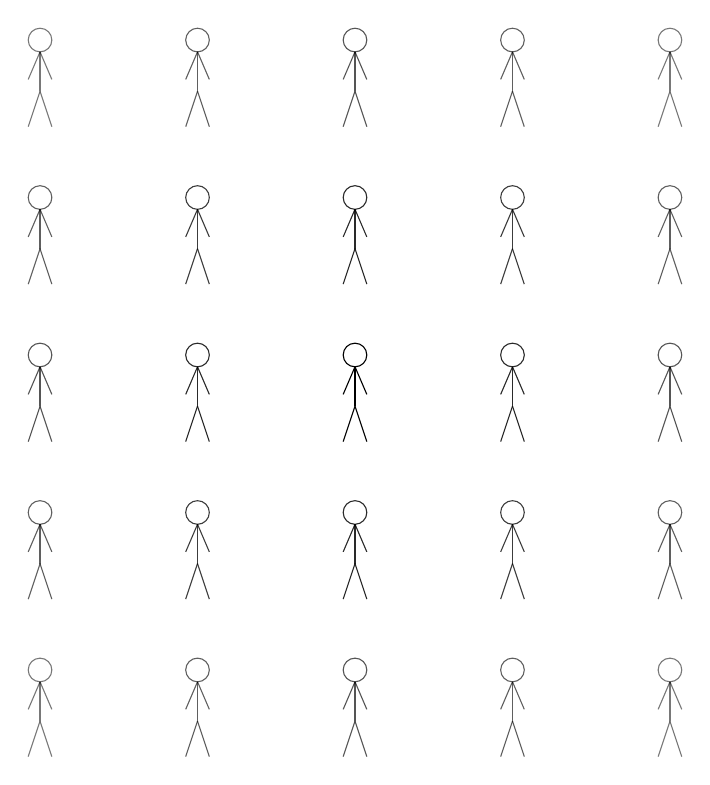
\begin{tikzpicture}
    \foreach \x in {-2,-1,...,2} {
      \foreach \y in {-2,-1,...,2} {
        \pgfmathsetmacro\c{1 - sqrt((\x)^2 + (\y)^2)/6};
        \begin{scope}[shift={(\x * 2, \y * 2)}, opacity=\c]
          \draw (0, 0.4) circle [radius=0.15];
          \draw (0, 0.25) -- (0, -0.25);
          \draw (0, -0.25) -- (-0.15, -0.7);
          \draw (0, -0.25) -- (0.15, -0.7);
          \draw (0, 0.25) -- (-0.15, -0.1);
          \draw (0, 0.25) -- (0.15, -0.1);
        \end{scope}
      }
    }
  \end{tikzpicture}
\end{center}
As we said, this looks somewhat likes $\R^2$, but we \emph{know} that this is not $\R^2$, since we can see some symmetry in this space. Whenever we move one unit horizontally or vertically, we get back to ``the same place''. In fact, we can move horizontally by $n$ units and vertically by $m$ units, for any $n, m \in \Z$, and still get back to the same place. This space has a huge translation symmetry. What is this symmetry? It is exactly $\Z \times \Z$.

We see that if we live inside the torus $S^1 \times S^1$, it feels like we are actually living in the universal covering space $\R \times \R$, except that we have an additional symmetry given by the fundamental group $\Z \times \Z$.

Hopefully, you are convinced that universal covers are nice. We would like to say that universal covers always exist. However, this is not always true.

Firstly, we should think --- what would having a universal cover imply? Suppose $X$ has a universal cover $\tilde{X}$. Pick any point $x_0 \in X$, and pick an evenly covered neighbourhood $U$ in $X$. This lifts to some $\tilde{U} \subseteq \tilde{X}$. If we draw a teeny-tiny loop $\gamma$ around $x_0$ inside $U$, we can lift this $\gamma$ to $\tilde{\gamma}$ in $\tilde{U}$. But we know that $\tilde{X}$ is simply connected. So $\tilde{\gamma}$ is homotopic to the constant path. Hence $\gamma$ is also homotopic to the constant path. So all loops (contained in $U$) at $x_0$ are homotopic to the constant path.

It seems like for every $x_0 \in X$, there is some neighbourhood of $x_0$ that is simply connected. Except that's not what we just showed above. The homotopy from $\tilde{\gamma}$ to the constant path is a homotopy in $\tilde{X}$, and can pass through anything in $\tilde{X}$, not just $\tilde{U}$. Hence the homotopy induced in $X$ is also a homotopy in $X$, not a homotopy in $U$. So $U$ itself need not be simply connected. What we have is a slightly weaker notion.

\begin{defi}[Locally simply connected]
  $X$ is \emph{locally simply connected} if for all $x_0\in X$, there is some neighbourhood $U$ of $x_0$ such that $U$ is simply connected.
\end{defi}

As we mentioned, what we actually want is a weaker condition.
\begin{defi}[Semi-locally simply connected]
  $X$ is \emph{semi-locally simply connected} if for all $x_0 \in X$, there is some neighbourhood $U$ of $x_0$ such that any loop $\gamma$ based at $x_0$ is homotopic to $c_{x_0}$ as paths \emph{in $X$}.
\end{defi}

We have just argued that if a universal cover $p: \tilde{X} \to X$ exists, then $X$ is semi-locally simply connected. This is really not interesting, since we don't care if a space is semi-locally simply connected. What is important is that this is the other direction. We still need one more additional condition:

\begin{defi}[Locally path connected]
  A space $X$ is \emph{locally path connected} if for any point $x$ and any neighbourhood $V$ of $x$, there is some open path connected $U \subseteq V$ such that $x \in U$.
\end{defi}

It is important to note that a path connected space need not be locally path connected. It is an exercise for the reader to come up with a counterexample.

\begin{thm}
  If $X$ is path connected, locally path connected and semi-locally simply connected, then $X$ has a universal covering.
\end{thm}
Note that we can alternatively define a universal covering as a covering space of $X$ that is also a covering space of all other covers of $X$. If we use this definition, then we can prove this result easily using Zorn's lemma. However, that proof is not too helpful since it does not tell us where the universal covering comes from. Instead, we will provide a constructive proof (sketch) that will hopefully be more indicative of what universal coverings are like.

\begin{proof}(idea)
  We pick a basepoint $x_0 \in X$ for ourselves. Suppose we have a universal covering $\tilde{X}$. Then this lifts to some $\tilde{x}_0$ in $\tilde{X}$. If we have any other point $\tilde{x} \in \tilde{X}$, since $\tilde{X}$ should be path connected, there is a path $\tilde{\alpha}: \tilde{x}_0 \rightsquigarrow \tilde{x}$. If we have another path, then since $\tilde{X}$ is simply connected, the paths are homotopic. Hence, we can identify each point in $\tilde{X}$ with a path from $\tilde{x}_0$, i.e.
  \[
    \{\text{points of }\tilde{X}\} \longleftrightarrow \{\text{paths }\tilde{\alpha}\text{ from }\tilde{x}_0\in \tilde{X}\}/{\simeq}.
  \]
  This is not too helpful though, since we are defining $\tilde{X}$ in terms of things in $\tilde{X}$. However, by path lifting, we know that paths $\tilde{\alpha}$ from $\tilde{x}_0$ in $\tilde{X}$ biject with paths $\alpha$ from $x_0$ in $X$. Also, by homotopy lifting, homotopies of paths in $X$ can be lifted to homotopies of paths in $\tilde{X}$. So we have
  \[
    \{\text{points of }\tilde{X}\} \longleftrightarrow \{\text{paths }\alpha\text{ from }x_0 \in X\}/{\simeq}.
  \]
  So we can produce our $\tilde{X}$ by picking a basepoint $x_0 \in X$, and defining
  \[
    \tilde{X} = \{\text{paths }\alpha: I\to X\text{ such that }\alpha(0) = x_0\}/{\simeq}.
  \]
  The covering map $p: \tilde{X} \to X$ is given by $[\alpha] \mapsto \alpha(1)$.

  One then has to work hard to define the topology, and then show this is simply connected. % complete!!!
\end{proof}

\subsection{The Galois correspondence}
Recall that at the beginning, we wanted to establish a correspondence between covering spaces and fundamental groups. We have already established the result that covering maps are injective on $\pi_1$. Therefore, given a (based) covering space $p: (\tilde{X}, \tilde{x}_0) \to (X, x_0)$, we can give a subgroup $p_*\pi_1(\tilde{X}, \tilde{x}_0)\leq \pi_1(X, x_0)$. It turns out that as long as we define carefully what we mean for based covering spaces to be ``the same'', this is a one-to-one correspondence --- each subgroup corresponds to a covering space.

We can have the following table of correspondences:
\begin{center}
  \begin{tabular}{rcl}
    \textbf{Covering spaces} & & \textbf{Fundamental group}\\
    (Based) covering spaces & $\longleftrightarrow$ & Subgroups of $\pi_1$\\
    Number of sheets & $\longleftrightarrow$ & Index\\
    Universal covers & $\longleftrightarrow$ & Trivial subgroup\\
  \end{tabular}
\end{center}
We now want to look at some of these correspondences.

Recall that we have shown that $\pi_1(X, x_0)$ acts on $p^{-1}(x_0)$. However, this is not too interesting an action, since $p^{-1}(x_0)$ is a discrete group with no structure. Having groups acting on a cube is fun because the cube has some structure. So we want something more ``rich'' for $\pi_1(X, x_0)$ to act on.

We note that we can make $\pi_1(X, x_0)$ ``act on'' the universal cover. How? Recall that in the torus example, each item in the fundamental group corresponds to translating the whole universal covering by some amount. In general, a point on $\tilde{X}$ can be thought of as a path $\alpha$ on $X$ starting from $x_0$. Then it is easy to make a loop $\gamma: x_0 \leadsto x_0$ act on this: use the concatenation $\gamma\cdot \alpha$: $[\gamma]\cdot [\alpha] = [\gamma \cdot \alpha]$.
\begin{center}
  \begin{tikzpicture}
    \draw plot [smooth cycle] coordinates {(-1.2, -0.7) (0, -0.7) (0.7, -1) (1.3, -0.9) (1.4, 0.4) (0.3, 1) (-1.7, 0.6)};

    \begin{scope}[shift={(-1, 3)}]
      \draw plot [smooth cycle] coordinates {(-1, -0.7) (0, -0.7) (1.2, -1) (2.6, -0.9) (3, 0.4) (0.6, 1) (-1.3, 0.6)};
      \node [below] at (-0.5, 0) {$\tilde{x}_0$};
      \node [below] at (0.8, 0.1) {$\tilde{x}_0'$};
      \draw (-0.5, 0) parabola (0.8, 0.1) node [pos=0.5, below] {$\tilde{\gamma}$};

      \node [circ] at (-0.5, 0) {};
      \node [circ] at (0.8, 0.1) {};

      \draw plot [smooth] coordinates {(0.8, 0.1) (1.3, 0.2) (1.8, 0.1)};
      \node [circ] at (1.8, 0.1) {};
      \node [above] at (1.3, 0.2) {$\alpha$};
    \end{scope}

    \draw [->] (3, 2.5) node [above] {\Large $\tilde{X}$} -- +(0, -2.2) node [below] {\Large $X$} node [pos=0.5, right] {$p$};

    \node [circ] at (0, 0) {};
    \node [below] at (0, 0) {$x_0$};

    \draw plot [tension=0.9, smooth] coordinates {(0, 0) (-1, -0.3) (-1.2, 0) (-0.8, 0.3) (0, 0)};
    \node at (-0.8, 0.3) [above] {$\gamma$};

    \draw plot [smooth] coordinates {(0, 0) (0.5, 0.1) (1, 0)};
    \node [circ] at (1, 0) {};
    \node [above] at (0.5, 0.1) {$\alpha$};
  \end{tikzpicture}
\end{center}
We will use this idea and return to the initial issue of making subgroups correspond to covering spaces. We want to show that this is surjective --- every subgroup arises from some cover. We want to say ``For any subgroup $H \leq \pi_1(X, x_0)$, there is a based covering map $p: (\tilde{X}, \tilde{x}_0)\to (X, x_0)$ such that $p_* \pi_1(\tilde{X}, \tilde{x}_0) = H$''. Except, this cannot possibly be true, since by taking the trivial subgroup, this would imply that there is a universal covering for every space. So we need some additional assumptions.

\begin{prop}
  Let $X$ be a path connected, locally path connected and semi-locally simply connected space. For any subgroup $H \leq \pi_1(X, x_0)$, there is a based covering map $p: (\tilde{X}, \tilde{x}_0)\to (X, x_0)$ such that $p_* \pi_1(\tilde{X}, \tilde{x}_0) = H$.
\end{prop}

\begin{proof}
  Since $X$ is a path connected, locally path connected and semi-locally simply connected space, let $\bar{X}$ be a universal covering. We have an intermediate group $H$ such that $\pi_1(\tilde{X}, \tilde{x}_0) = 1 \leq H \leq \pi_1(X, x_0)$. How can we obtain a corresponding covering space?

  Note that if we have $\bar{X}$ and we want to recover $X$, we can quotient $\bar{X}$ by the action of $\pi_1(X, x_0)$. Since $\pi_1(X, x_0)$ acts on $\bar{X}$, so does $H \leq \pi_1(X, x_0)$. Now we can define our covering space by taking quotients. We define $\sim_H$ on $\bar{X}$ to be the orbit relation for the action of $H$, i.e.\ $\tilde{x} \sim_H \tilde{y}$ if there is some $h \in H$ such that $\tilde{y} = h\tilde{x}$. We then let $\tilde{X}$ be the quotient space $\bar{X}/{\sim_H}$.

  We can now do the messy algebra to show that this is the covering space we want. % complete again
\end{proof}
We have just showed that every subgroup comes from some covering space, i.e.\ the map from the set of covering spaces to the subgroups of $\pi_1$ is surjective. Now we want to prove injectivity. To do so, we need a generalization of the homotopy lifting lemma.

Suppose we have path-connected spaces $(Y, y_0)$, $(X, x_0)$ and $(\tilde{X}, \tilde{x}_0)$, with $f: (Y, y_0) \to (X, x_0)$ a continuous map, $p: (\tilde{X}, \tilde{x}_0) \to (X, x_0)$ a covering map. When does a lift of $f$ to $\tilde{f}: (Y, y_0) \to (\tilde{X}, \tilde{x}_0)$ exist? The answer is given by the lifting criterion.

\begin{lemma}[Lifting criterion]
  Let $p: (\tilde{X}, \tilde{x}_0) \to (X, x_0)$ be a covering map of path-connected based spaces, and $(Y, y_0)$ a path-connected, locally path connected based space. If $f: (Y, y_0) \to (X, x_0)$ is a continuous map, then there is a (unique) lift $\tilde{f}: (Y, y_0) \to (\tilde{X}, \tilde{x}_0)$ such that the diagram below commutes (i.e.\ $p\circ \tilde{f} = f$):
  \[
    \begin{tikzcd}[row sep=large]
      & (\tilde{X}, \tilde{x}_0) \ar[d, "p"]\\
      (Y, y_0) \ar [r, "f"'] \ar [ru, dashed, "\tilde{f}"] & (X, x_0)
    \end{tikzcd}
  \]
  if and only if the following condition holds:
  \[
    f_* \pi_1(Y, y_0) \leq p_*\pi_1(\tilde{X}, \tilde{x}_0).
  \]
\end{lemma}
Note that uniqueness comes from the uniqueness of lifts. So this lemma is really about existence.

Also, note that the condition holds trivially when $Y$ is simply connected, e.g.\ when it is an interval (path lifting) or a square (homotopy lifting). So paths and homotopies can always be lifted.

\begin{proof}
  One direction is easy: if $\tilde{f}$ exists, then $f = p \circ \tilde{f}$. So $f_* = p_* \circ \tilde{f}_*$. So we know that $\im f_* \subseteq \im p_*$. So done.

  In the other direction, uniqueness follows from the uniqueness of lifts. So we only need to prove existence. We define $\tilde{f}$ as follows:

  Given a $y \in Y$, there is some path $\alpha_y: y_0 \leadsto y$. Then $f$ maps this to $\beta_y: x_0 \leadsto f(y)$ in $X$. By path lifting, this path lifts uniquely to $\tilde{\beta}_y$ in $\tilde{X}$. Then we set $\tilde{f}(y) = \tilde{\beta}_y(1)$. Note that if $\tilde{f}$ exists, then this \emph{must} be what $\tilde{f}$ sends $y$ to. What we need to show is that this is well-defined.

  Suppose we picked a different path $\alpha'_y: y_0 \leadsto y$. Then this $\alpha_y'$ would have differed from $\alpha_y$ by a loop $\gamma$ in $Y$.

  Our condition that $f_* \pi_1(Y, y_0) \leq p_*\pi_1(\tilde{X}, \tilde{x}_0)$ says $f\circ \gamma$ is the image of a loop in $\tilde{X}$. So $\tilde{\beta}_y$ and $\tilde{\beta}'_y$ also differ by a loop in $\tilde{X}$, and hence have the same end point. So this shows that $\tilde{f}$ is well-defined.

  Finally, we show that $\tilde{f}$ is continuous. First, observe that any open set $U \subseteq \tilde{X}$ can be written as a union of $\tilde{V}$ such that $p|_{\tilde{V}}: \tilde{V} \to p(\tilde{V})$ is a homeomorphism. Thus, it suffices to show that if $p|_{\tilde{V}}: \tilde{V} \to p(\tilde{V}) = V$ is a homeomorphism, then $\tilde{f}^{-1}(\tilde{V})$ is open.

  Let $y \in \tilde{f}^{-1}(\tilde{V})$, and let $x = f(y)$. Since $f^{-1}(V)$ is open and $Y$ is locally path-connected, we can pick an open $W \subseteq f^{-1}(V)$ such that $y \in W$ and $W$ is path connected. We claim that $W \subseteq \tilde{f}^{-1}(\tilde{V})$.

  Indeed, if $z \in W$, then we can pick a path $\gamma$ from $y$ to $z$. Then $f$ sends this to a path from $x$ to $f(z)$. The lift of this path to $\tilde{X}$ is given by $p|_{\tilde{V}}^{-1} (f(\gamma))$, whose end point is $p|_{\tilde{V}}^{-1}(f(z)) \in \tilde{V}$. So it follows that $\tilde{f}(z) = p|_{\tilde{V}}^{-1}(f(z)) \in \tilde{V}$.

\end{proof}

Now we prove that every subgroup of $\pi_1$ comes from exactly one covering space. What this statement properly means is made precise in the following proposition:
\begin{prop}
  Let $(X, x_0)$, $(\tilde{X}_1, \tilde{x}_1)$, $(\tilde{X}_2, \tilde{X}_2)$ be path-connected based spaced, and $p_i: (\tilde{X}_i, \tilde{x}_i) \to (X, x_0)$ be covering maps. Then we have
  \[
    p_{1*}\pi_1(\tilde{X}_1, \tilde{x}_1) = p_{2*} \pi_1(\tilde{X}_2, \tilde{x_2})
  \]
  if and only if there is some \emph{homeomorphism} $h$ such that the following diagram commutes:
  \[
    \begin{tikzcd}[row sep=large, column sep=tiny]
      (\tilde{X}_1, \tilde{x}_1) \ar[rr, dashed, "h"] \ar[rd, "p_1"'] & & (\tilde{X}_2, \tilde{x}_2) \ar[ld, "p_2"]\\
      & (X, x_0)
    \end{tikzcd}
  \]
  i.e.\ $p_1 = p_2 \circ h$.
\end{prop}
Note that this is a stronger statement than just saying the two covering spaces are homeomorphic. We are saying that we can find a nice homeomorphism that works well with the covering map $p$.

\begin{proof}
  If such a homeomorphism exists, then clearly the subgroups are equal. If the subgroups are equal, we rotate our diagram a bit:
  \[
    \begin{tikzcd}[row sep=large]
      & (\tilde{X}_2, \tilde{x}_2) \ar[d, "p_2"]\\
      (\tilde{X}_1, \tilde{x}_1) \ar [r, "p_1"'] \ar [ru, dashed, "h = \tilde{p}_1"] & (X, x_0)
    \end{tikzcd}
  \]
  Then $h = \tilde{p}_1$ exists by the lifting criterion. By symmetry, we can get $h^{-1} = \tilde{p}_2$. To show $\tilde{p}_2$ is indeed the inverse of $\tilde{p}_1$, note that $\tilde{p}_2 \circ \tilde{p}_1$ is a lift of $p_2 \circ \tilde{p}_1 = p_1$. Since $\id_{\tilde{X}_1}$ is also a lift, by the uniqueness of lifts, we know $\tilde{p}_2 \circ \tilde{p}_1$ is the identity map. Similarly, $\tilde{p}_1 \circ \tilde{p}_2$ is also the identity.
  \[
    \begin{tikzcd}[row sep=large]
      & & (\tilde{X}_1, \tilde{x}_1) \ar[d, "p_1"]\\
      (\tilde{X}_1, \tilde{x}_1) \ar[rr, bend right, "p_1"'] \ar [r, "\tilde{p}_1"'] & (\tilde{X}_2, \tilde{x}_2) \ar [ru, "\tilde{p}_2"] \ar[r, "p_2"'] & (X, x_0)
    \end{tikzcd}%\qedhere
  \]
\end{proof}
Now what we would like to do is to forget about the basepoints. What happens when we change base points? Recall that the effect of changing base points is that we will conjugate our group. This doesn't actually change the group itself, but if we are talking about subgroups, conjugation can send a subgroup into a different subgroup. Hence, if we do not specify the basepoint, we don't get a subgroup of $\pi_1$, but a \emph{conjugacy class} of subgroups.

\begin{prop}
  Unbased covering spaces correspond to conjugacy classes of subgroups.
\end{prop}

\section{Some group theory}
Algebraic topology is about translating topology into group theory. Unfortunately, you don't know group theory. Well, maybe you do, but not the right group theory. So let's learn group theory!

\subsection{Free groups and presentations}
Recall that in IA Groups, we defined, say, the dihedral group to be
\[
  D_{2n} = \bra r, s \mid r^n = s^2 = e, srs = r^{-1}\ket.
\]
What does this expression actually mean? Can we formally assign a meaning to this expression?

We start with a simple case --- the free group. This is, in some sense, the ``freest'' group we can have. It is defined in terms of an alphabet and words.

\begin{defi}[Alphabet and words]
 We let $S = \{s_\alpha: \alpha \in \Lambda\}$ be our \emph{alphabet}, and we have an extra set of symbols $S^{-1} = \{s_\alpha^{-1}: \alpha \in \Lambda\}$. We assume that $S\cap S^{-1} = \emptyset$. What do we do with alphabets? We write words with them!

 We define $S^*$ to be the set of \emph{words} over $S\cup S^{-1}$, i.e.\ it contains $n$-tuples $x_1 \cdots x_n$ for any $0 \leq n < \infty$, where each $x_i \in S \cup S^{-1}$.
\end{defi}

\begin{eg}
  Let $S = \{a, b\}$. Then words could be the empty word $\emptyset$, or $a$, or $aba^{-1}b^{-1}$, or $aa^{-1}aaaaabbbb$, etc. We are usually lazy and write $aa^{-1}aaaaabbbb$ as $aa^{-1}a^5 b^4$.
\end{eg}

When we see things like $aa^{-1}$, we would want to cancel them. This is called \emph{elementary reduction}.
\begin{defi}[Elementary reduction]
  An \emph{elementary reduction} takes a word $us_\alpha s_\alpha^{-1}v$ and gives $uv$, or turns $us_\alpha^{-1}s_\alpha v$ into $uv$.
\end{defi}
Since each reduction shortens the word, and the word is finite in length, we cannot keep reducing for ever. Eventually, we reach a \emph{reduced} state.

\begin{defi}[Reduced word]
  A word is \emph{reduced} if it does not admit an elementary reduction.
\end{defi}

\begin{eg}
  $\emptyset$, $a$, $aba^{-1}b^{-1}$ are reduced words, while $aa^{-1}aaaaabbbb$ is not.
\end{eg}
Note that there is an inclusion map $S \to S^*$ that sends the symbol $s_\alpha$ to the word $s_\alpha$.

\begin{defi}[Free group]
  The \emph{free group} on the set $S$, written $F(S)$, is the set of reduced words on $S^*$ together with some operations:
  \begin{enumerate}
    \item Multiplication is given by concatenation followed by elementary reduction to get a reduced word. For example, $(aba^{-1}b^{-1}) \cdot (bab) = aba^{-1}b^{-1}bab = ab^2$
    \item The identity is the empty word $\emptyset$.
    \item The inverse of $x_1\cdots x_n$ is $x_n^{-1}\cdots x_1^{-1}$, where, of course, $(s_\alpha^{-1})^{-1} = s_\alpha$.
  \end{enumerate}
  The elements of $S$ are called the \emph{generators} of $F(S)$.
\end{defi}
Note that we have not showed that multiplication is well-defined --- we might reduce the same word in different ways and reach two different reduced words. We will show that this is indeed well-defined later, using topology!

Some people like to define the free group in a different way. This is a cleaner way to define the free group without messing with alphabets and words, but is (for most people) less intuitive. This definition also does not make it clear that the free group $F(S)$ of any set $S$ exists. We will state this definition as a lemma.
\begin{lemma}
  If $G$ is a group and $\phi: S\to G$ is a set map, then there exists a unique \emph{homomorphism} $f: F(S) \to G$ such that the following diagram commutes:
  \[
    \begin{tikzcd}
      F(S) \ar[dr, dashed, "f"] \\
      S \ar[u] \ar[r, "\phi"'] & G
    \end{tikzcd}
  \]
  where the arrow not labeled is the natural inclusion map that sends $s_\alpha$ (as a symbol from the alphabet) to $s_\alpha$ (as a word).
\end{lemma}

\begin{proof}
  Clearly if $f$ exists, then $f$ must send each $s_\alpha$ to $\phi(s_\alpha)$ and $s_\alpha^{-1}$ to $\phi(s_\alpha)^{-1}$. Then the values of $f$ on all other elements must be determined by
  \[
    f(x_1\cdots x_n) = f(x_1)\cdots f(x_n)
  \]
  since $f$ is a homomorphism. So if $f$ exists, it must be unique. So it suffices to show that this $f$ is a well-defined homomorphism.

  This is well-defined if we define $F(S)$ to be the set of all reduced words, since each reduced word has a unique representation (since it is \emph{defined} to be the representation itself).

  To show this is a homomorphism, suppose
  \[
    x = x_1\cdots x_n a_1\cdots a_k,\quad y = a_k^{-1} \cdots a_1^{-1} y_1\cdots y_m,
  \]
  where $y_1 \not= x_n^{-1}$. Then
  \[
    xy = x_1 \cdots x_n y_1\cdots y_m.
  \]
  Then we can compute
  \begin{align*}
    f(x)f(y) &= \big(\phi(x_1)\cdots \phi(x_n) \phi(a_1) \cdots \phi(a_k)\big) \big(\phi(a_k)^{-1} \cdots \phi(a_1)^{-1}\phi(y_1)\cdots\phi(y_m)\big) \\
    &= \phi(x_1)\cdots\phi(x_n) \cdots \phi(y_1)\cdots \phi(y_m) \\
    &= f(xy).
  \end{align*}
  So $f$ is a homomorphism.
\end{proof}
We call this a ``universal property'' of $F(S)$. We can show that $F(S)$ is the unique group satisfying the conditions of this lemma (up to isomorphism), by taking $G = F(S)$ and using the uniqueness properties.

\begin{defi}[Presentation of a group]
  Let $S$ be a set, and let $R \subseteq F(S)$ be any sub\emph{set}. We denote by $\bra \bra R\ket\ket$ the \emph{normal closure} of $R$, i.e.\ the smallest normal subgroup of $F(S)$ containing $R$. This can be given explicitly by
  \[
    \bra \bra R\ket \ket = \left\{\prod_{i = 1}^n g_i r_i g_i^{-1}: n \in \N, r_i \in R, g_i \in F(S)\right\}.
  \]
  Then we write
  \[
    \bra S \mid R\ket = F(S)/\bra\bra R\ket\ket.
  \]
\end{defi}
This is just the usual notation we have for groups. For example, we can write
\[
  D_{2n} = \bra r, s \mid r^n, s^2, srsr\ket.
\]
Again, we can define this with a universal property.
\begin{lemma}
  If $G$ is a group and $\phi: S \to G$ is a set map such that $f(r) = 1$ for all $r \in R$ (i.e.\ if $r = s_1^{\pm 1}s_2^{\pm 1}\cdots s_m^{\pm 1}$, then $\phi(r) = \phi(s_1)^{\pm 1}\phi(s_2)^{\pm 1} \cdots \phi(s_m)^{\pm 1} = 1$), then there exists a unique homomorphism $f: \bra S \mid R\ket \to G$ such that the following triangle commutes:
  \[
    \begin{tikzcd}
      \bra S\mid R\ket \ar[dr, dashed, "f"] \\
      S \ar[u] \ar[r, "\phi"'] & G
    \end{tikzcd}
  \]
\end{lemma}
Proof is similar to the previous one.

In some sense, this says that all the group $\bra S\mid R \ket$ does is it satisfies the relations in $R$, and nothing else.

\begin{eg}[The \st{stupid} canonical presentation]
  Let $G$ be a group. We can view the group as a set, and hence obtain a free group $F(G)$. There is also an obvious surjection $G \to G$. Then by the universal property of the free group, there is a surjection $f: F(G) \to G$. Let $R = \ker f = \bra \bra R\ket \ket$. Then $\bra G \mid R \ket$ is a presentation for $G$, since the first isomorphism theorem says
  \[
    G \cong F(G) / \ker f.
  \]
\end{eg}
This is a really stupid example. For example, even the simplest non-trivial group $\Z/2$ will be written as a quotient of a free group with two generators. However, this tells us that every group has a presentation.

\begin{eg}
  $\bra a, b\mid b \ket \cong \bra a\ket \cong \Z$.
\end{eg}

\begin{eg}
  With a bit of work, we can show that $\bra a, b\mid ab^{-3}, ba^{-2}\ket = \Z/5$.
\end{eg}

\subsection{Another view of free groups}
Recall that we have not yet properly defined free groups, since we did not show that multiplication is well-defined. We are now going to do this using topology.

Again let $S$ be a set. For the following illustration, we will just assume $S = \{ a, b\}$, but what we will do works for any set $S$. We define $X$ by
\begin{center}
  \begin{tikzpicture}[scale=0.75]
    \draw (-1, 0) circle [radius=1];
    \draw (1, 0) circle [radius=1];
    \node [circ] {};
    \node [left] at (-2, 0) {$a$};
    \node [right] at (2, 0) {$b$};
    \draw [->] (2, 0.1) -- (2, 0.11);
    \draw [->] (-2, 0.1) -- (-2, 0.11);
    \node [right] {$x_0$};
  \end{tikzpicture}
\end{center}
We call this a ``rose with 2 petals''. This is a cell complex, with one $0$-cell and $|S|$ 1-cells. For each $s \in S$, we have one $1$-cell, $e_s$, and we fix a path $\gamma_s: [0, 1] \to e_s$ that goes around the 1-cell once. We will call the $0$-cells and $1$-cells \emph{vertices} and \emph{edges}, and call the whole thing a \emph{graph}.

What's the universal cover of $X$? Since we are just lifting a $1$-complex, the result should be a $1$-complex, i.e.\ a graph. Moreover, this graph is connected and simply connected, i.e.\ it's a tree. We also know that every vertex in the universal cover is a copy of the vertex in our original graph. So it must have 4 edges attached to it. So it has to look like something this:
\begin{center}
  \begin{tikzpicture}[scale=0.5]
    \draw (-3, 0) -- (3, 0);
    \draw (0, -3) -- (0, 3);
    \foreach \x/\y/\rot in {3/0/0, 0/3/90, -3/0/180, 0/-3/270} {
      \begin{scope}[shift={(\x, \y)}, scale=0.5, rotate=\rot]
        \draw (0, 0) -- (3, 0);
        \draw (0, 3) -- (0, -3);
        \foreach \x/\y/\rot in {3/0/0, 0/3/90, 0/-3/270} {
          \begin{scope}[shift={(\x, \y)}, scale=0.5, rotate=\rot]
            \draw (0, 0) -- (3, 0);
            \draw (0, 3) -- (0, -3);
            \foreach \x/\y/\rot in {3/0/0, 0/3/90, 0/-3/270} {
              \begin{scope}[shift={(\x, \y)}, scale=0.5, rotate=\rot]
                \draw (0, 0) -- (3, 0);
                \draw (0, 3) -- (0, -3);
                \foreach \x/\y/\rot in {3/0/0, 0/3/90, 0/-3/270} {
                  \begin{scope}[shift={(\x, \y)}, scale=0.5, rotate=\rot]
                    \draw (0, 0) -- (3, 0);
                    \draw (0, 3) -- (0, -3);
                    \foreach \x/\y/\rot in {3/0/0, 0/3/90, 0/-3/270} {
                      \begin{scope}[shift={(\x, \y)}, scale=0.5, rotate=\rot]
                        \draw (0, 0) -- (3, 0);
                        \draw (0, 3) -- (0, -3);
                      \end{scope}
                    }
                  \end{scope}
                }
              \end{scope}
            }
          \end{scope}
        }
      \end{scope}
    }
    \node [circ] {};
    \node [anchor = south west] {$\tilde{x}_0$};
  \end{tikzpicture}
\end{center}
In $X$, we know that at each vertex, there should be an edge labeled $a$ going in; an edge labeled $a$ going out; an edge labeled $b$ going in; an edge labeled $b$ going out. This should be the case in $\tilde{X}$ as well. So $\tilde{X}$ looks like this:
\begin{center}
  \begin{tikzpicture}[scale=0.5]
    \draw (-3, 0) -- (3, 0);
    \draw (0, -3) -- (0, 3);
    \foreach \x/\y/\rot in {3/0/0, 0/3/90, -3/0/180, 0/-3/270} {
      \begin{scope}[shift={(\x, \y)}, scale=0.5, rotate=\rot]
        \draw (0, 0) -- (3, 0);
        \draw (0, 3) -- (0, -3);
        \foreach \x/\y/\rot in {3/0/0, 0/3/90, 0/-3/270} {
          \begin{scope}[shift={(\x, \y)}, scale=0.5, rotate=\rot]
            \draw (0, 0) -- (3, 0);
            \draw (0, 3) -- (0, -3);
            \foreach \x/\y/\rot in {3/0/0, 0/3/90, 0/-3/270} {
              \begin{scope}[shift={(\x, \y)}, scale=0.5, rotate=\rot]
                \draw (0, 0) -- (3, 0);
                \draw (0, 3) -- (0, -3);
                \foreach \x/\y/\rot in {3/0/0, 0/3/90, 0/-3/270} {
                  \begin{scope}[shift={(\x, \y)}, scale=0.5, rotate=\rot]
                    \draw (0, 0) -- (3, 0);
                    \draw (0, 3) -- (0, -3);
                    \foreach \x/\y/\rot in {3/0/0, 0/3/90, 0/-3/270} {
                      \begin{scope}[shift={(\x, \y)}, scale=0.5, rotate=\rot]
                        \draw (0, 0) -- (3, 0);
                        \draw (0, 3) -- (0, -3);
                      \end{scope}
                    }
                  \end{scope}
                }
              \end{scope}
            }
          \end{scope}
        }
      \end{scope}
    }
    \node [circ] {};
    \node [anchor = south west] {$\tilde{x}_0$};
    \draw [->] (1.7, 0) -- (1.71, 0);
    \node [above] at (1.5, 0) {$a$};
    \draw [->] (-1.3, 0) -- (-1.29, 0);
    \node [above] at (-1.5, 0) {$a$};

    \draw [->] (0, 1.7) -- (0, 1.71);
    \node [left] at (0, 1.5) {$b$};
    \draw [->] (0, -1.3) -- (0, -1.29);
    \node [left] at (0, -1.5) {$b$};

    \draw [->] (3.9, 0) -- (4, 0);
    \node [above] at (3.75, 0) {$a$};

    \draw [->] (3, 0.9) -- (3, 1);
    \node [left] at (3, 0.75) {$b$};
    \draw [->] (3, -0.5) -- (3, -0.4);
    \node [left] at (3, -0.75) {$b$};
  \end{tikzpicture}
\end{center}
The projection map is then obvious --- we send all the vertices in $\tilde{X}$ to $x_0 \in X$, and then the edges according to the labels they have, in a way that respects the direction of the arrow. It is easy to show this is really a covering map.

We are now going to show that this tree ``is'' the free group. Notice that every word $w \in S^*$ denotes a unique ``edge path'' in $\tilde{X}$ starting at $\tilde{x}_0$, where an edge path is a sequence of oriented edges $\tilde{e}_1, \cdots, \tilde{e}_n$ such that the ``origin'' of $\tilde{e}_{i + 1}$ is equal to the ``terminus'' of $\tilde{e}_i$.

For example, the following path corresponds to $w = abb^{-1}b^{-1}b a^{-1}b^{-1}$.
\begin{center}
  \begin{tikzpicture}[scale=0.5]
    \draw (-3, 0) -- (3, 0);
    \draw (0, -3) -- (0, 3);
    \foreach \x/\y/\rot in {3/0/0, 0/3/90, -3/0/180, 0/-3/270} {
      \begin{scope}[shift={(\x, \y)}, scale=0.5, rotate=\rot]
        \draw (0, 0) -- (3, 0);
        \draw (0, 3) -- (0, -3);
        \foreach \x/\y/\rot in {3/0/0, 0/3/90, 0/-3/270} {
          \begin{scope}[shift={(\x, \y)}, scale=0.5, rotate=\rot]
            \draw (0, 0) -- (3, 0);
            \draw (0, 3) -- (0, -3);
            \foreach \x/\y/\rot in {3/0/0, 0/3/90, 0/-3/270} {
              \begin{scope}[shift={(\x, \y)}, scale=0.5, rotate=\rot]
                \draw (0, 0) -- (3, 0);
                \draw (0, 3) -- (0, -3);
                \foreach \x/\y/\rot in {3/0/0, 0/3/90, 0/-3/270} {
                  \begin{scope}[shift={(\x, \y)}, scale=0.5, rotate=\rot]
                    \draw (0, 0) -- (3, 0);
                    \draw (0, 3) -- (0, -3);
                    \foreach \x/\y/\rot in {3/0/0, 0/3/90, 0/-3/270} {
                      \begin{scope}[shift={(\x, \y)}, scale=0.5, rotate=\rot]
                        \draw (0, 0) -- (3, 0);
                        \draw (0, 3) -- (0, -3);
                      \end{scope}
                    }
                  \end{scope}
                }
              \end{scope}
            }
          \end{scope}
        }
      \end{scope}
    }
    \node [circ] {};
    \node [anchor = south west] {$\tilde{x}_0$};
    \draw [mred, ->-=0.1, ->-=0.45, ->-=0.7, ->-=0.9] (0, 0.1) -- (2.9, 0.1) -- (2.9, 1.5) -- (3.1, 1.5) -- (3.1, -1.5) -- (2.9, -1.5) -- (2.9, -0.1) -- (0.1, -0.1) -- (0.1, -3);
  \end{tikzpicture}
\end{center}
We can note a few things:
\begin{enumerate}
  \item $\tilde{X}$ is connected. So for all $\tilde{x} \in p^{-1}(x_0)$, there is an edge-path $\tilde{\gamma}: \tilde{x}_0 \leadsto \tilde{x}$.
  \item If an edge-path $\tilde{\gamma}$ fails to be locally injective, we can simplify it. How can an edge fail to be locally injective? It is fine if we just walk along a path, since we are just tracing out a line. So it fails to be locally injective if two consecutive edges in the path are the same edge with opposite orientations:
    \begin{center}
      \begin{tikzpicture}
        \draw [->-=0.16, ->-=0.9] (-1, 0) -- (-0.05, 0) node [pos=0.5, below] {$\tilde{e}_{i - 1}$} -- (-0.05, 1) node [pos=0.5, left] {$\tilde{e}_{i}$} -- (0.05, 1) -- (0.05, 0) node [pos=0.5, right] {$\tilde{e}_{i + 1}$} -- (1, 0) node [pos=0.5, below] {$\tilde{e}_{i+2}$};
      \end{tikzpicture}
    \end{center}
    We can just remove the redundant lines and get
    \begin{center}
      \begin{tikzpicture}
        \draw [->-=0.3, ->-=0.85] (-1, 0) -- (0, 0) node [pos=0.5, below] {$\tilde{e}_{i - 1}$} -- (1, 0) node [pos=0.5, below] {$\tilde{e}_{i + 2}$};
      \end{tikzpicture}
    \end{center}
    This reminds us of two things --- homotopy of paths \emph{and} elementary reduction of words.
  \item Each point $\tilde{x} \in p^{-1}(x_0)$ is joined to $\tilde{x}_0$ by a \emph{unique} locally injective edge-path.
  \item For any $w \in S^*$, from (ii), we know that $\tilde{\gamma}$ is locally injective if and only if $w$ is reduced.
\end{enumerate}
We can thus conclude that there are bijections
\[
  \begin{tikzcd}
    F(S) & p^{-1}(x_0) \ar[l] \ar [r] & \pi_1(X, x_0)
  \end{tikzcd}
\]
that send $\tilde{x}$ to the word $w \in F(S)$ such that $\tilde{\gamma}_w$ is a locally injective edge-path to $\tilde{x}_0 \leadsto \tilde{x}$; and $\tilde{x}$ to $[\gamma] \in \pi_1(X, x_0)$ such that $\tilde{x}_0 \cdot [\gamma] = \tilde{x}$.

So there is a bijection between $F(S)$ and $\pi_1(X, x_0)$. It is easy to see that the operations on $F(S)$ and $\pi_1(X, x_0)$ are the same, since they are just concatenating words or paths. So this bijection identifies the two group structures. So this induces an isomorphism $F(S)\cong \pi_1(X, x_0)$.

\subsection{Free products with amalgamation}
We managed to compute the fundamental group of the circle. But we want to find the fundamental group of more things. Recall that at the beginning, we defined cell complexes, and said these are the things we want to work with. Cell complexes are formed by gluing things together. So we want to know what happens when we glue things together.

Suppose a space $X$ is constructed from two spaces $A, B$ by gluing (i.e.\ $X = A\cup B$). We would like to describe $\pi_1(X)$ in terms of $\pi_1(A)$ and $\pi_1(B)$. To understand this, we need to understand how to ``glue'' groups together.

\begin{defi}[Free product]
  Suppose we have groups $G_1 = \bra S_1 \mid R_1\ket, G_2 = \bra S_2 \mid R_2\ket$, where we assume $S_1 \cap S_2 = \emptyset$. The \emph{free product} $G_1 * G_2$ is defined to be
  \[
    G_1 * G_2 = \bra S_1 \cup S_2 \mid R_1 \cup R_2\ket.
  \]
\end{defi}
This is not a really satisfactory definition. A group can have many different presentations, and it is not clear this is well-defined. However, it is clear that this group exists. Note that there are natural homomorphisms $j_i: G_i \to G_1 * G_2$ that send generators to generators. Then we can have the following universal property of the free product:

\begin{lemma}
  $G_1 * G_2$ is the group such that for any group $K$ and homomorphisms $\phi_i: G_i \to K$, there exists a unique homomorphism $f: G_1 * G_2 \to K$ such that the following diagram commutes:
  \[
    \begin{tikzcd}[row sep=large]
      & G_2 \ar[rdd, bend left, "\phi_2"] \ar[d, "j_2"]\\
      G_1 \ar[rrd, bend right, "\phi_1"] \ar [r, "j_1"] & G_1 * G_2 \ar [rd, dashed, "f"]\\
      && K
    \end{tikzcd}
  \]
\end{lemma}

\begin{proof}
  It is immediate from the universal property of the definition of presentations.
\end{proof}

\begin{cor}
  The free product is well-defined.
\end{cor}

\begin{proof}
  The conclusion of the universal property can be seen to characterize $G_1 * G_2$ up to isomorphism.
\end{proof}

Again, we have a definition in terms of a concrete construction of the group, without making it clear this is well-defined; then we have a universal property that makes it clear this is well-defined, but not clear that the object actually exists. Combining the two would give everything we want.

However, this free product is not exactly what we want, since there is little interaction between $G_1$ and $G_2$. In terms of gluing spaces, this corresponds to gluing $A$ and $B$ when $A \cap B$ is trivial (i.e.\ simply connected). What we really need is the free product with amalgamation, as you might have guessed from the title.

\begin{defi}[Free product with amalgamation]
  Suppose we have groups $G_1$, $G_2$ and $H$, with the following homomorphisms:
  \[
    \begin{tikzcd}[row sep=large]
      H \ar[r, "i_2"] \ar[d, "i_1"] & G_2\\
      G_1
    \end{tikzcd}
  \]
  The \emph{free product with amalgamation} is defined to be
  \[
    G_1 \underset{H}{*} G_2 = G_1 * G_2/ \bra \bra \{(j_2 \circ i_2(h))^{-1} (j_1 \circ i_1)(h): h\in H\}\ket \ket.
  \]
\end{defi}
Here we are attempting to identify things ``in $H$'' as the same, but we need to use the maps $j_k$ and $i_k$ to map the things from $H$ to $G_1 * G_2$. So we want to say ``for any $h$, $j_1 \circ i_1 (h) = j_2 \circ i_2(h)$'', or $(j_2 \circ i_2(h))^{-1} (j_1 \circ i_1)(h) = e$. So we quotient by the (normal closure) of these things.

We have the universal property
\begin{lemma}
  $G_1 \underset{H}{*} G_2$ is the group such that for any group $K$ and homomorphisms $\phi_i: G_i \to K$, there exists a unique homomorphism $G_1 \underset{H}{*} G_2 \to K$ such that the following diagram commutes:
  \[
    \begin{tikzcd}[row sep=large]
      H \ar[r, "i_2"] \ar[d, "i_1"] & G_2 \ar[rdd, bend left, "\phi_2"] \ar[d, "j_2"]\\
      G_1 \ar[rrd, bend right, "\phi_1"] \ar [r, "j_1"] & G_1 \underset{H}{*} G_2 \ar [rd, dashed, "f"]\\
      && K
    \end{tikzcd}
  \]
\end{lemma}
This is the language we will need to compute fundamental groups. These definitions will (hopefully) become more concrete as we see more examples.
\section{Seifert-van Kampen theorem}
\subsection{Seifert-van Kampen theorem}
The Seifert-van Kampen theorem is the theorem that tells us what happens when we glue spaces together.

Here we let $X = A\cup B$, where $A, B, A\cap B$ are path-connected.
\begin{center}
  \begin{tikzpicture}
    \draw [fill=mred, fill opacity=0.3] (-1, 0) ellipse (1.5 and 0.6);
    \draw [fill=mblue, fill opacity=0.3] (1, 0) ellipse (1.5 and 0.6);
    \node [circ] {};
    \node [above] {$x_0$};
    \node at (-2.5, 0.6) {$A$};
    \node at (2.5, 0.6) {$B$};
  \end{tikzpicture}
\end{center}
We pick a basepoint $x_0 \in A\cap B$ for convenience. Since we like diagrams, we can write this as a commutative diagram:
\[
  \begin{tikzcd}[row sep=large]
    A\cap B \ar [r, hook] \ar[d, hook] & B\ar[d, hook]\\
    A \ar [r, hook] & X
  \end{tikzcd}
\]
where all arrows are inclusion (i.e.\ injective) maps. We can consider what happens when we take the fundamental groups of each space. Then we have the induced homomorphisms
\[
  \begin{tikzcd}[row sep=large]
    \pi_1(A\cap B, x_0) \ar [r] \ar[d] & \pi_1(B, x_0)\ar[d]\\
    \pi_1(A, x_0) \ar [r] & \pi_1(X, x_0)
  \end{tikzcd}
\]
We might guess that $\pi_1(X, x_0)$ is just the free product with amalgamation
\[
  \pi_1(X, x_0) = \pi_1(A, x_0) \underset{\pi_1(A\cap B, x_0)}{*} \pi_1(B, x_0).
\]
The Seifert-van Kampen theorem says that, under mild hypotheses, this guess is correct.

\begin{thm}[Seifert-van Kampen theorem]
  Let $A, B$ be open subspaces of $X$ such that $X = A\cup B$, and $A, B, A\cap B$ are path-connected. Then for any $x_0 \in A\cap B$, we have
  \[
    \pi_1(X, x_0) = \pi_1(A, x_0) \underset{\pi_1(A\cap B, x_0)}{*} \pi_1(B, x_0).
  \]
\end{thm}
Note that by the universal property of the free product with amalgamation, we by definition know that there is a unique map $\pi_1(A, x_0) \underset{\pi_1(A\cap B, x_0)}{*} \pi_1(B, x_0) \to \pi_1(X, x_0)$. The theorem asserts that \emph{this} map is an isomorphism.

Proof is omitted because time is short. % put proof.

\begin{eg}
  Consider a higher-dimensional sphere $S^n = \{\mathbf{v} \in \R^{n + 1}: |\mathbf{v}| = 1\}$ for $n \geq 2$. We want to find $\pi_1(S^n)$.

  The idea is to write $S^n$ as a union of two open sets. We let $n = \mathbf{e}_1 \in S^n \subseteq \R^{n + 1}$ be the North pole, and $s = -\mathbf{e}_1$ be the South pole. We let $A = S^n \setminus \{n\}$, and $B = S^n \setminus\{s\}$. By stereographic projection, we know that $A, B \cong \R^n$. The hard part is to understand the intersection.

  To do so, we can draw a cylinder $S^{n - 1} \times (-1, 1)$, and project our $A\cap B$ onto the cylinder. We can similarly project the cylinder onto $A\cap B$. So $A\cap B\cong S^{n - 1} \times (-1, 1) \simeq S^{n - 1}$, since $(-1, 1)$ is contractible.
  \begin{center}
    \begin{tikzpicture}
      \draw circle [radius=2];
      \draw [dashed] (2, 0) arc (0:180:2 and 0.3);
      \draw (-2, 0) arc (180:360:2 and 0.3);

      \node [circ] at (0, 2) {};
      \node [circ] at (0, -2) {};

      \node [above] at (0, 2) {$n$};
      \node [below] at (0, -2) {$s$};

      \draw [mblue, shading=axis, left color=mblue, right color=mblue!60!white, fill opacity=0.2] (-2, -2) -- (-2, 2) arc (180:360:2 and 0.3) -- (2, -2) arc (360:180:2 and 0.3);
      \draw [mblue] (2, 2) arc (0:180:2 and 0.3);
      \draw [mblue, dashed] (2, -2) arc (0:180:2 and 0.3);
    \end{tikzpicture}
  \end{center}
  We can now apply the Seifert-van Kampen theorem. Note that this works only if $S^{n - 1}$ is path-connected, i.e.\ $n \geq 2$. Then this tells us that
  \[
    \pi_1(S^n) \cong \pi_1(\R^n) \underset{\pi_1(S^{n - 1})}{*} \pi_1(\R^n) \cong 1 \underset{\pi_1(S^{n - 1})}{*} 1
  \]
  It is easy to see this is the trivial group. We can see this directly form the universal property of the amalgamated free product, or note that it is the quotient of $1 * 1$, which is $1$.

  So for $n \geq 2$, $\pi_1(S^n) \cong 1$.
\end{eg}
We have found yet another simply connected space. However, this is unlike our previous examples. Our previous spaces were simply connected because they were contractible. However, we will later see that $S^n$ is not contractible. So this is genuinely a new, interesting example.

Why did we go though all this work to prove that $\pi_1(S^n) \cong 1$? It feels like we can just prove this directly --- pick a point that is not in the curve as the North pole, project stereographically to $\R^n$, and contract it there. However, the problem is that space-filling curves exist. We cannot guarantee that we can pick a point not on the curve! It is indeed possible to prove directly that given any curve on $S^n$ (with $n \geq 1$), we can deform it slightly so that it is no longer surjective. Then the above proof strategy works. However, using Seifert-van Kampen is much neater.

\begin{eg}[$\RP^n$]
  Recall that $\RP^n \cong S^n/\{\pm \id\}$, and the quotient map $S^n \to \RP^n$ is a covering map. Now that we have proved that $S^n$ is simply connected, we know that $S^n$ is a universal cover of $\RP^n$.

  For any $x_0 \in \RP^n$, we have a bijection
  \[
    \pi_1(\RP^n, x_0) \leftrightarrow p^{-1}(x_0).
  \]
  Since $p^{-1}(x_0)$ has two elements by definition, we know that $|\pi_1(\RP^n, x_0)| = 2$. So $\pi_1(\RP^n, x_0) = \Z/2$.
\end{eg}
You will prove a generalization of this in example sheet 2.

\begin{eg}[Wedge of two circles]
  We are going to consider the operation of \emph{wedging}. Suppose we have two topological spaces, and we want to join them together. The natural way to join them is to take the disjoint union. What if we have based spaces? If we have $(X, x_0)$ and $(Y, y_0)$, we cannot just take the disjoint union, since we will lose our base point. What we do is take the \emph{wedge sum}, where we take the disjoint union and then identify the base points:
  \begin{center}
    \begin{tikzpicture}
      \node [above] at (-1.5, 1) {$X$};
      \node [above] at (1.5, 1) {$Y$};
      \draw [fill=mblue, fill opacity=0.2] (-1.5, 0) circle [radius=1];
      \draw [fill=mred, fill opacity=0.2] (1.5, 0) circle [radius=1];

      \node [circ] at (-0.5, 0) {};
      \node [circ] at (0.5, 0) {};

      \node [left] at (-0.5, 0) {$x_0$};
      \node [right] at (0.5, 0) {$y_0$};

      \draw [->] (0, -1.5) -- (0, -2.5);
      \begin{scope}[shift={(0, -4)}]
        \node [right] at (2, 0) {$X\wedge Y$};
        \draw [fill=mblue, fill opacity=0.2] (-1, 0) circle [radius=1];
        \draw [fill=mred, fill opacity=0.2] (1, 0) circle [radius=1];

        \node [circ] {};
        \node [left] {$x_0 \sim y_0$};
      \end{scope}
    \end{tikzpicture}
  \end{center}
  Suppose we take the wedge sum of two circles $S^1 \wedge S^1$. We would like to pick $A, B$ to be each of the circles, but we cannot, since $A$ and $B$ have to be open. So we take slightly more, and get the following:
  \begin{center}
    \begin{tikzpicture}[scale=0.75]
      \draw (-1, 0) circle [radius=1];
      \draw (1, 0) circle [radius=1];
      \node [circ] {};
      \node [right] {$x_0$};
      \draw [mred] (-1, 0) circle [radius=1.2];
      \draw [mblue] (1, 0) circle [radius=1.2];
      \node [below, mred] at (-1, -1.2) {$A$};
      \node [below, mblue] at (1, -1.2) {$B$};
    \end{tikzpicture}
  \end{center}
  Each of $A$ and $B$ now look like this:
  \begin{center}
    \begin{tikzpicture}[scale=0.75]
      \draw (0, 0) circle [radius=1];
      \draw (1, 0) arc (180:150:1);
      \draw (1, 0) arc (180:210:1);
      \node [circ] at (1, 0) {};
    \end{tikzpicture}
  \end{center}
  We see that both $A$ and $B$ retract to the circle. So $\pi_1(A) \cong \pi_1(B) \cong \Z$, while $A\cap B$ is a cross, which retracts to a point. So $\pi_1 (A\cap B) = 1$.

  Hence by the Seifert-van Kampen theorem, we get
  \[
    \pi_1(S^1 \wedge S^1, x_0) = \pi_1(A, x_0)\underset{\pi_1(A\cap B, x_0)}{*} \pi_1(B, x_0) \cong \Z \underset{1}{*} \Z \cong \Z * \Z \cong F_2,
  \]
  where $F_2$ is just $F(S)$ for $|S| = 2$. We can see that $\Z*\Z \cong F_2$ by showing that they satisfy the same universal property.

  Note that we had already figured this out when we studied the free group, where we realized $F_2$ is the fundamental group of this thing.

  More generally, as long as $x_0, y_0$ in $X$ and $Y$ are ``reasonable'', $\pi_1(X\wedge Y) \cong \pi_1(X) * \pi_1(Y)$.
\end{eg}

Next, we would exhibit some nice examples of the covering spaces of $S^1 \wedge S^1$, i.e.\ the ``rose with 2 petals''.

Recall that $\pi_1(S^1 \wedge S^1, x_0) \cong F_2 \cong \bra a, b\ket$.

\begin{eg}
  Consider the map $\phi: F_2 \to \Z/3$ which sends $a \mapsto 1, b \mapsto 1$. Note that $1$ is \emph{not} the identity, since this is an abelian group, and the identity is $0$. This exists since the universal property tells us we just have to say where the generators go, and the map exists (and is unique).

  Now $\ker\phi$ is a subgroup of $F_2$. So there is a based covering space of $S^1 \wedge S^1$ corresponding to it, say, $\tilde{X}$. Let's work out what it is.

  First, we want to know how many sheets it has, i.e.\ how many copies of $x_0$ we have. There are three, since we know that the number of sheets is the index of the subgroup, and the index of $\ker \phi$ is $|\Z/3| = 3$ by the first isomorphism theorem.
  \begin{center}
    \begin{tikzpicture}
      \node [circ] at (0, 1) {};
      \node [circ] at (0, -1) {};
      \node [circ] at (1.87, 0) {};
      \node [right] at (1.87, 0) {$\tilde{x}_0$};
    \end{tikzpicture}
  \end{center}
  Let's try to lift the loop $a$ at $\tilde{x}_0$. Since $a \not\in \ker\phi = \pi_1(\tilde{X}, \tilde{x}_0)$, $a$ does not lift to a loop. So it goes to another vertex.
  \begin{center}
    \begin{tikzpicture}
      \node [circ] at (0, 1) {};
      \node [circ] at (0, -1) {};
      \node [circ] at (1.87, 0) {};
      \node [right] at (1.87, 0) {$\tilde{x}_0$};

      \draw [->] (1.87, 0) -- (0, -1) node [pos=0.5, below] {$a$};
    \end{tikzpicture}
  \end{center}
  Similarly, $a^2 \not\in \ker\phi = \pi_1(\tilde{X}, \tilde{x}_0)$. So we get the following
  \begin{center}
    \begin{tikzpicture}
      \node [circ] at (0, 1) {};
      \node [circ] at (0, -1) {};
      \node [circ] at (1.87, 0) {};
      \node [right] at (1.87, 0) {$\tilde{x}_0$};

      \draw [->] (1.87, 0) -- (0, -1) node [pos=0.5, below] {$a$};
      \draw [->] (0, -1) -- (0, 1) node [pos=0.5, left] {$a$};
    \end{tikzpicture}
  \end{center}
  Since $a^3 \in \ker \phi$, we get a loop labelled $a$.
  \begin{center}
    \begin{tikzpicture}
      \node [circ] at (0, 1) {};
      \node [circ] at (0, -1) {};
      \node [circ] at (1.87, 0) {};
      \node [right] at (1.87, 0) {$\tilde{x}_0$};

      \draw [->] (1.87, 0) -- (0, -1) node [pos=0.5, below] {$a$};
      \draw [->] (0, -1) -- (0, 1) node [pos=0.5, left] {$a$};
      \draw [->] (0, 1) -- (1.87, 0) node [pos=0.5, above] {$a$};
    \end{tikzpicture}
  \end{center}
  Note that $ab^{-1} \in \ker \phi$. So $ab^{-1}$ gives a loop. So $b$ goes in the same direction as $a$:
  \begin{center}
    \begin{tikzpicture}
      \node [circ] at (0, 1) {};
      \node [circ] at (0, -1) {};
      \node [circ] at (1.87, 0) {};
      \node [right] at (1.87, 0) {$\tilde{x}_0$};

      \draw [->] (1.87, 0) -- (0, -1) node [pos=0.5, above] {$a$};
      \draw [->] (0, -1) -- (0, 1) node [pos=0.5, right] {$a$};
      \draw [->] (0, 1) -- (1.87, 0) node [pos=0.5, below] {$a$};

      \draw (1.87, 0) to [bend left, ->] node [pos=0.5, below] {$b$} (0, -1);
      \draw (0, -1) edge [bend left, ->] node [pos=0.5, left] {$b$} (0, 1);
      \draw (0, 1) edge [bend left, ->] node [pos=0.5, above] {$b$} (1.87, 0);
    \end{tikzpicture}
  \end{center}
  This is our covering space.
\end{eg}
This is a fun game to play at home:
\begin{enumerate}
  \item Pick a group $G$ (finite groups are recommended).
  \item Then pick $\alpha, \beta\in G$ and let $\phi: F_2 \to G$ send $a \mapsto \alpha, b \mapsto \beta$.
  \item Compute the covering space corresponding to $\phi$.
\end{enumerate}

\subsection{The effect on \texorpdfstring{$\pi_1$}{pi1} of attaching cells}
We have started the course by talking about cell complexes, but largely ignored them afterwards. Finally, we are getting back to them.

The process of attaching cells is as follows: we start with a space $X$, get a function $S^{n - 1} \to X$, and attach $D^n$ to $X$ by gluing along the image of $f$ to get $X\cup_f D^n$:
\begin{center}
  \begin{tikzpicture}[scale=2]
    \draw ellipse (0.3 and 0.5);

    \draw [thick, mred, decorate, decoration={snake, segment length=1cm}] circle [radius=0.2];

    \draw [thick, mred] (2, 0.3) arc (90:270:0.1 and 0.3);
    \draw [dashed, thick, mred] (2, -0.3) arc (270:450:0.1 and 0.3);

    \fill [mblue, opacity=0.3] (2, 0.3) arc (90:270:0.1 and 0.3) arc (270:450:0.3);
    \draw [thick, mblue] (2, -0.3) arc (270:450:0.3);

    \draw [dashed] (2, 0.3) -- (0, 0.4);
    \draw [dashed] (2, -0.3) -- (0.1, -0.23);

    \node [circ] at (2.3, 0) {};
    \node [right] at (2.3, 0) {$0$};

    \node [circ] at (1.9, 0) {};
    \node [left] at (1.9, 0) {$y_0$};

    \node [circ] at (-0.19, 0) {};
    \node [left] at (-0.19, 0) {$x_0$};
  \end{tikzpicture}
\end{center}
Since we are attaching stuff, we can use the Seifert-van Kampen theorem to analyse this.
\begin{thm}
  If $n \geq 3$, then $\pi_1(X\cup_f D^n) \cong \pi_1(X)$. More precisely, the map $\pi_1(X, x_0) \to \pi_1(X\cup_f D^n, x_0)$ induced by inclusion is an isomorphism, where $x_0$ is a point on the image of $f$.
\end{thm}
This tells us that attaching a high-dimensional disk does not do anything to the fundamental group.

\begin{proof}
  Again, the difficulty of applying Seifert-van Kampen theorem is that we need to work with open sets.

  Let $0 \in D^n$ be any point in the interior of $D^n$. We let $A = X\cup_f (D^n \setminus \{0\})$. Note that $D^n \setminus \{0\}$ deformation retracts to the boundary $S^{n - 1}$. So $A$ deformation retracts to $X$. Let $B = \mathring{D}$, the interior of $D^n$. Then
  \[
    A\cap B = \mathring{D}^n \setminus 0 \cong S^{n - 1}\times (-1, 1)
  \]
  We cannot use $y_0$ as our basepoint, since this point is not in $A\cap B$. Instead, pick an arbitrary $y_1 \in A\cap B$. Since $D^n$ is path connected, we have a path $\gamma: y_1 \leadsto y_0$, and we can use this to recover the fundamental groups based at $y_0$.

  Now Seifert-van Kampen theorem says
  \[
    \pi_1(X\cup_f D^n, y_1) \cong \pi_1(A, y_1) \underset{\pi_1(A\cap B, y_1)}{*} \pi_1(B, y_1).
  \]
  Since $B$ is just a disk, and $A\cap B$ is simply connected ($n \geq 3$ implies $S^{n - 1}$ is simply connected), their fundamental groups are trivial. So we get
  \[
    \pi_1(X\cup_f D^n, y_1) \cong \pi_1(A, y_1).
  \]
  We can now use $\gamma$ to change base points from $y_1$ to $y_0$. So
  \[
    \pi_1(X\cup_f D^n, y_0) \cong \pi_1(A, y_0) \cong \pi_1(X, y_0).\qedhere
  \]
\end{proof}
The more interesting case is when we have smaller dimensions.
\begin{thm}
  If $n = 2$, then the natural map $\pi_1(X, X_0) \to \pi_1(X\cup_f D^n, x_0)$ is \emph{surjective}, and the kernel is $\bra\bra [f] \ket \ket$. Note that this statement makes sense, since $S^{n - 1}$ is a circle, and $f: S^{n - 1} \to X$ is a loop in $X$.
\end{thm}
This is what we would expect, since if we attach a disk onto the loop given by $f$, this loop just dies.

\begin{proof}
  As before, we get
  \[
    \pi_1(X\cup_f D^n, y_1) \cong \pi_1(A, y_1) \underset{\pi_1(A\cap B, y_1)}{*} \pi_1(B, y_1).
  \]
  Again, $B$ is contractible, and $\pi_1(B, y_1) \cong 1$. However, $\pi_1(A\cap B, y_1) \cong \Z$. Since $\pi_1(A\cap B, y_1)$ is just (homotopic to) the loop induced by $f$, it follows that
  \[
    \pi_1(A, y_1) \underset{\pi_1(A\cap B, y_1)}{*} 1 = (\pi_1(A, y_1) * 1)/\bra \bra \pi_1(A\cap B, y_1)\ket \ket \cong \pi_1(X, x_0)/\bra \bra f\ket\ket.\qedhere
  \]
\end{proof}

In summary, we have
\[
  \pi_1(X \cup_f D^n) =
  \begin{cases}
    \pi_1(X) & n \geq 3\\
    \pi_1(X)/\bra\bra f\ket\ket & n = 2
  \end{cases}
\]
This is a useful result, since this is how we build up cell complexes. If we want to compute the fundamental groups, we can just work up to the two-cells, and know that the higher-dimensional cells do not have any effect. Moreover, whenever $X$ is a cell complex, we should be able to write down the presentation of $\pi_1(X)$.

\begin{eg}
  Let $X$ be the $2$-torus. Possibly, our favorite picture of the torus is (not a doughnut):
  \begin{center}
    \begin{tikzpicture}
      \draw [->-=0.55, mred] (0, 0) -- (3, 0);
      \draw [->-=0.55, mred] (0, 3) -- (3, 3);

      \draw [->-=0.55, mblue] (0, 0) -- (0, 3);
      \draw [->-=0.55, mblue] (3, 0) -- (3, 3);
    \end{tikzpicture}
  \end{center}
  This is already a description of the torus as a cell complex!

  We start with our zero complex $X^{(0)}$:
  \begin{center}
    \begin{tikzpicture}
      \node [circ] {};
    \end{tikzpicture}
  \end{center}
  We then add our $1$-cells to get $X^{(1)}$:
  \begin{center}
    \begin{tikzpicture}
      \node [circ] {};
      \draw [mred] (1, 0) ellipse (1 and 0.4);
      \draw [mblue] (-0.5, 0) circle [radius=0.5];

      \draw [->, mred] (1, -0.4) -- (1.01, -0.4);
      \draw [->, mblue] (-1, 0) -- (-1, 0.01);
      \node [right, mred] at (2, 0) {$a$};
      \node [left, mblue] at (-1, 0) {$b$};
    \end{tikzpicture}
  \end{center}
  We now glue our square to the cell complex to get $X = X^{(2)}$:
  \begin{center}
    \begin{tikzpicture}[scale=0.75]
      \draw [->-=0.55, mred] (0, 0) -- (3, 0);
      \draw [->-=0.55, mred] (0, 3) -- (3, 3);

      \draw [->-=0.55, mblue] (0, 0) -- (0, 3);
      \draw [->-=0.55, mblue] (3, 0) -- (3, 3);
    \end{tikzpicture}
  \end{center}
  matching up the colors and directions of arrows.

  So we have our torus as a cell complex. What is its fundamental group? There are many ways we can do this computation, but this time we want to do it as a cell complex.

  We start with $X^{(0)}$. This is a single point. So its fundamental group is $\pi_1(X^{(0)}) = 1$.

  When we add our two 1-cells, we get $\pi_1(X^{(1)}) = F_2 \cong \bra a, b\ket$.

  Finally, to get $\pi_1(X)$, we have to quotient out by the boundary of our square, which is just $aba^{-1}b^{-1}$. So we have
  \[
    \pi_1(X^{(2)}) = F_2/\bra \bra aba^{-1}b^{-1}\ket\ket = \bra a, b \mid aba^{-1}b^{-1}\ket \cong \Z^2.
  \]
  We have the last congruence since we have two generators, and then we make them commute by quotienting the commutator out.
\end{eg}
This procedure can be reversed --- given a presentation of a group, we can just add the right edges and squares to produce a cell complex with that presentation.

\begin{cor}
  For any (finite) group presentation $\bra S\mid R\ket$, there exists a (finite) cell complex (of dimension 2) $X$ such that $\pi_1(X) \cong \bra S\mid R \ket$.
\end{cor}
There really isn't anything that requires that finiteness in this proof, but finiteness makes us feel more comfortable.

\begin{proof}
  Let $S = \{a_1, \cdots, a_m\}$ and $R = \{r_1, \cdots, r_n\}$. We start with a single point, and get our $X^{(1)}$ by adding a loop about the point for each $a_i \in S$. We then get our $2$-cells $e_j^2$ for $j = 1, \cdots, n$, and attaching them to $X^{(1)}$ by $f_i: S^1 \to X^{(1)}$ given by a based loop representing $r_i \in F(S)$.
\end{proof}
Since all groups have presentations, this tells us that all groups are fundamental groups of some spaces (at least those with finite presentations).

\subsection{A refinement of the Seifert-van Kampen theorem}
We are going to make a refinement of the theorem so that we don't have to worry about that openness problem. We first start with a definition.

\begin{defi}[Neighbourhood deformation retract]
  A subset $A\subseteq X$ is a \emph{neighbourhood deformation retract} if there is an open set $A\subseteq U\subseteq X$ such that $A$ is a strong deformation retract of $U$, i.e.\ there exists a retraction $r: U \to A$ and $r \simeq \id_U \rel A$.
\end{defi}
This is something that is true most of the time, in sufficiently sane spaces.

\begin{eg}
  If $Y$ is a subcomplex of a cell complex, then $Y$ is a neighbourhood deformation retract.
\end{eg}

\begin{thm}
  Let $X$ be a space, $A, B\subseteq X$ closed subspaces. Suppose that $A$, $B$ and $A\cap B$ are path connected, and $A\cap B$ is a neighbourhood deformation retract of $A$ and $B$. Then for any $x_0 \in A\cap B$.
  \[
    \pi_1(X, x_0) = \pi_1(A, x_0) \underset{\pi_1(A\cap B, x_0)}{*} \pi_1(B, x_0).
  \]
\end{thm}
\begin{center}
  \begin{tikzpicture}
    \draw [fill=mred, fill opacity=0.3] (-1, 0) ellipse (1.5 and 0.6);
    \draw [fill=mblue, fill opacity=0.3] (1, 0) ellipse (1.5 and 0.6);
    \node [circ] {};
    \node [above] {$x_0$};
    \node at (-2.5, 0.6) {$A$};
    \node at (2.5, 0.6) {$B$};
  \end{tikzpicture}
\end{center}
This is just like Seifert-van Kampen theorem, but usually easier to apply, since we no longer have to ``fatten up'' our $A$ and $B$ to make them open.

\begin{proof}
  Pick open neighbourhoods $A\cap B \subseteq U \subseteq A$ and $A \cap B \subseteq V \subseteq B$ that strongly deformation retract to $A\cap B$. Let $U$ be such that $U$ retracts to $A \cap B$. Since $U$ retracts to $A$, it follows that $U$ is path connected since path-connectedness is preserved by homotopies.

  Let $A' = A \cup V$ and $B' = B \cup U$. Since $A' = (X \setminus B) \cup V$, and $B' = (X \setminus A) \cup U$, it follows that $A'$ and $B'$ are open.

  Since $U$ and $V$ retract to $A \cap B$, we know $A' \simeq A$ and $B' \simeq B$. Also, $A' \cap B' = (A \cup V) \cap (B \cup U) = U \cup V \simeq A \cap B$. In particular, it is path connected. So by Seifert van-Kampen, we get
  \[
    \pi_1(A \cup B) = \pi_1(A', x_0) \underset{\pi_1(A' \cap B', x_0)}{*} \pi_1(B', x_0) = \pi_1(A, x_0) \underset{\pi_1(A\cap B, x_0)}{*} \pi_1(B, x_0).\qedhere
  \]
\end{proof}
This is basically what we've done all the time when we enlarge our $A$ and $B$ to become open.

\begin{eg}
  Let $X = S^1 \wedge S^1$, the rose with two petals. Let $A, B\cong S^1$ be the circles.
  \begin{center}
    \begin{tikzpicture}[scale=0.75]
      \draw [mred] (-1, 0) circle [radius=1];
      \draw [mblue] (1, 0) circle [radius=1];
      \node [circ] {};
      \node [right] {$x_0$};
      \node [below, mred] at (-1, -1) {$A$};
      \node [below, mblue] at (1, -1) {$B$};
    \end{tikzpicture}
  \end{center}
  Then since $\{x_0\} = A \cap B$ is a neighbourhood deformation retract of $A$ and $B$, we know that
  \[
    \pi_1 X \cong \pi_1 S^1 * \pi_1S^1.
  \]
\end{eg}
\subsection{The fundamental group of all surfaces}
We have found that the torus has fundamental group $\Z^2$, but we already knew this, since the torus is just $S^1 \times S^1$, and the fundamental group of a product is the product of the fundamental groups, as you have shown in the example sheet. So we want to look at something more interesting. We look at \emph{all} surfaces.

We start by defining what a surface is. It is surprisingly difficult to get mathematicians to agree on how we can define a surface. Here we adopt the following definition:
\begin{defi}[Surface]
  A \emph{surface} is a Hausdorff topological space such that every point has a neighbourhood $U$ that is homeomorphic to $\R^2$.
\end{defi}
Some people like $\C$ more that $\R$, and sometimes they put $\C^2$ instead of $\R^2$ in the definition, which is confusing, since that would have two complex dimensions and hence \emph{four} real dimensions. Needless to say, the actual surfaces will also be different and have different homotopy groups. We will just focus on surfaces with two real dimensions.

To find the fundamental group of all surfaces, we rely on the following theorem that tells us what surfaces there are.
\begin{thm}[Classification of compact surfaces]
  If $X$ is a compact surface, then $X$ is homeomorphic to a space in one of the following two families:
  \begin{enumerate}
    \item The \emph{orientable surface of genus $g$}, $\Sigma_g$ includes the following (please excuse my drawing skills):
      \begin{center} % improve
        \begin{tikzpicture}
          \begin{scope}
            \draw circle [radius=1];
            \draw [dashed] (1, 0) arc (0:180:1 and 0.25);
            \draw (-1, 0) arc (180:360:1 and 0.25);
          \end{scope}

          \begin{scope}[shift={(3, 0)}]
            \draw (0,0) ellipse (1 and 0.56);
            \path[rounded corners=12pt] (-0.45, 0)--(0, 0.3)--(0.45, 0) (-0.45, 0)--(0, -0.28)--(0.45, 0);
            \draw[rounded corners=14pt] (-0.55, 0.05)--(0, -.15)--(0.55, 0.05);
            \draw[rounded corners=12pt] (-0.45, 0)--(0, 0.3)--(0.45, 0);
          \end{scope}

          \begin{scope}[shift={(6.5, 0)}, yscale=1.5]
            \draw plot [smooth cycle, tension=0.8] coordinates {(-1.7, 0) (-1.4, -0.27) (-0.7, -0.35) (0, -0.23) (0.7, -0.35) (1.4, -0.27) (1.7, 0) (1.4, 0.27) (0.7, 0.35) (0, 0.23) (-0.7, 0.35) (-1.4, 0.27)};

            \foreach \x in {0.8, -0.8}{
              \begin{scope}[shift={(\x, -0.03)}]
                \path[rounded corners=12pt] (-0.45, 0)--(0, 0.2)--(0.45, 0) (-0.45, 0)--(0, -0.28)--(0.45, 0);
                \draw[rounded corners=14pt] (-0.55, 0.05)--(0, -.15)--(0.55, 0.05);
                \draw[rounded corners=12pt] (-0.45, 0)--(0, 0.2)--(0.45, 0);
              \end{scope}
            }
        \end{scope}
        \end{tikzpicture}
      \end{center}
      A more formal definition of this family is the following: we start with the 2-sphere, and remove a few discs from it to get $S^2 \setminus \cup_{i = 1}^g D^2$. Then we take $g$ tori with an open disc removed, and attach them to the circles.
      \begin{center}
        \begin{tikzpicture}
          \draw circle [radius=2];
          \draw [dashed] (2, 0) arc (0:180:2 and 0.5);
          \draw (-2, 0) arc (180:360:2 and 0.5);

          \foreach \y/\r/\a/\b in {0.8/-60/1.573/1.23, -0.8/60/1.23/1.573} {
            \begin{scope}[shift={(0, \y)}]
              \draw [rotate around={\r:(1.4, 0)}, mblue, fill=mblue, fill opacity=0.5] (1.4, 0) ellipse (0.346 and 0.11);
              \draw [dashed] (\a, -0.3) -- (3.6, -0.3);
              \draw [dashed] (\b, 0.3) -- (3.6, 0.3);
              \begin{scope}[shift={(4.5, 0)}, xscale=0.75]
                \draw plot [smooth, tension=0.8] coordinates {(-1.2, 0.3) (-1, 0.3) (0, 0.56) (1, 0.3) (1, -0.3) (0, -0.56) (-1, -0.3) (-1.2, -0.3)};
                \draw [mblue, fill=mblue, fill opacity=0.5] (-1.2, 0) ellipse (0.1 and 0.3);
                \path[rounded corners=12pt] (-0.45, 0)--(0, 0.3)--(0.45, 0) (-0.45, 0)--(0, -0.28)--(0.45, 0);
                \draw[rounded corners=14pt] (-0.55, 0.05)--(0, -.15)--(0.55, 0.05);
                \draw[rounded corners=12pt] (-0.45, 0)--(0, 0.3)--(0.45, 0);
              \end{scope}
            \end{scope}
          }
        \end{tikzpicture}
      \end{center}

    \item The \emph{non-orientable surface of genus $n$}, $E_n = \{\RP^2, K, \cdots\}$ (where $K$ is the Klein bottle). This has a similar construction as above: we start with the sphere $S^2$, make a few holes, and then glue M\"obius strips to them.
  \end{enumerate}
\end{thm}
It would be nice to be able to compute fundamental groups of these guys. To do so, we need to write them as polygons with identification.

\begin{eg}
  To obtain a surface of genus two, written $\Sigma_2$, we start with what we had for a torus:
  \begin{center}
    \begin{tikzpicture}[rotate=22.5]
      \coordinate (0) at (1, 0);
      \coordinate (1) at (0, 0);
      \coordinate (2) at (-0.707, -0.707);
      \coordinate (3) at (-0.707, -1.707);
      \coordinate (4) at (0, -2.414);

      \draw [mred, ->-=0.6] (0) -- (1) node [above, pos=0.5] {$a$};
      \draw [mblue, ->-=0.6] (1) -- (2) node [left, pos=0.5] {$b$};
      \draw [mred, ->-=0.6] (3) -- (2) node [left, pos=0.5] {$a$};
      \draw [mblue, ->-=0.6] (4) -- (3) node [below, pos=0.5] {$b$};
    \end{tikzpicture}
  \end{center}
  If we just wanted a torus, we are done (after closing the loop), but now we want a surface with genus $2$, so we add another torus:
  \begin{center}
    \begin{tikzpicture}[rotate=22.5]
      \coordinate (0) at (1, 0);
      \coordinate (1) at (0, 0);
      \coordinate (2) at (-0.707, -0.707);
      \coordinate (3) at (-0.707, -1.707);
      \coordinate (4) at (0, -2.414);
      \coordinate (5) at (1, -2.414);
      \coordinate (6) at (1.707, -1.707);
      \coordinate (7) at (1.707, -0.707);

      \draw [mred, ->-=0.6] (0) -- (1) node [above, pos=0.5] {$a_1$};
      \draw [mblue, ->-=0.6] (1) -- (2) node [left, pos=0.5] {$b_1$};
      \draw [mred, ->-=0.6] (3) -- (2) node [left, pos=0.5] {$a_1$};
      \draw [mblue, ->-=0.6] (4) -- (3) node [below, pos=0.5] {$b_1$};

      \draw [mgreen, ->-=0.6] (4) -- (5) node [below, pos=0.5] {$a_2$};
      \draw [morange, ->-=0.6] (5) -- (6) node [right, pos=0.5] {$b_2$};
      \draw [mgreen, ->-=0.6] (7) -- (6) node [right, pos=0.5] {$a_2$};
      \draw [morange, ->-=0.6] (0) -- (7) node [above, pos=0.5] {$b_2$};

      \draw [dashed] (0) -- (4);
    \end{tikzpicture}
  \end{center}
  To visualize how this works, imagine cutting this apart along the dashed line. This would give two tori with a hole, where the boundary of the holes are just the dashed line. Then gluing back the dashed lines would give back our orientable surface with genus 2.
  \begin{center}
    \begin{tikzpicture}
      \foreach \x/\r in {2/1, -2/-1} {
        \begin{scope}[shift={(\x, 0)}, xscale=\r]
          \begin{scope}[xscale=0.75]
            \draw plot [smooth, tension=0.8] coordinates {(-1.2, 0.3) (-1, 0.3) (0, 0.56) (1, 0.3) (1, -0.3) (0, -0.56) (-1, -0.3) (-1.2, -0.3)};
            \draw [mblue, fill=mblue, fill opacity=0.5] (-1.2, 0) ellipse (0.1 and 0.3);
            \path[rounded corners=12pt] (-0.45, 0)--(0, 0.3)--(0.45, 0) (-0.45, 0)--(0, -0.28)--(0.45, 0);
            \draw[rounded corners=14pt] (-0.55, 0.05)--(0, -.15)--(0.55, 0.05);
            \draw[rounded corners=12pt] (-0.45, 0)--(0, 0.3)--(0.45, 0);
          \end{scope}
        \end{scope}
      }
      \draw [dashed] (-1.1, 0.3) -- (1.1, 0.3);
      \draw [dashed] (-1.1, -0.3) -- (1.1, -0.3);
    \end{tikzpicture}
  \end{center}
  In general, to produce $\Sigma_g$, we produce a polygon with $4g$ sides. Then we get
  \[
    \pi_1 \Sigma_g = \bra a_1, b_1, \cdots, a_g, b_g\mid a_1 b_1 a_1^{-1} b_1^{-1} \cdots a_g b_g a_g^{-1}b_g^{-1}\ket.
  \]
  We do we care? The classification theorem tells us that each surface is homeomorphic to \emph{some} of these orientable and non-orientable surfaces, but it doesn't tell us there is no overlap. It might be that $\Sigma_6\cong \Sigma_{241}$, via some weird homeomorphism that destroys some holes.

  However, this result lets us know that all these orientable surfaces are genuinely different. While it is difficult to stare at this fundamental group and say that $\pi_1 \Sigma_g \not\cong \pi_1 \Sigma_{g'}$ for $g\not= g'$, we can perform a little trick. We can take the abelianization of the group $\pi_1 \Sigma_g$, where we further quotient by all commutators. Then the abelianized fundamental group of $\Sigma_g$ will simply be $\Z^{2g}$. These are clearly distinct for different values of $g$. So all these surfaces are distinct. Moreover, they are not even homotopy equivalent.
\end{eg}

The fundamental groups of the non-orientable surfaces is left as an exercise for the reader. % complete ?

\section{Simplicial complexes}
So far, we have taken a space $X$, and assigned some things to it. The first was easy --- $\pi_0(X)$. It was easy to calculate and understand. We then spent a lot of time talking about $\pi_1(X)$. What are they good for? A question we motivated ourselves with was to prove $\R^m \cong \R^n$ implies $n = m$. $\pi_0$ was pretty good for the case when $n = 1$. If $\R^m \cong \R$, then we would have $\R^m \setminus \{0\} \cong \R\setminus \{0\} \simeq S^0$. We know that $|\pi_0(S^0)| = 2$, while $|\pi_0(\R^m \setminus \{0\})| = 1$ for $m \not= 1$. This is just a fancy way of saying that $\R \setminus \{0\}$ is disconnected while $\R^m \setminus \{0\}$ is not for $m \not= 1$.

We can just add $1$ to $n$, and add $1$ to our subscript. If $\R^m \cong \R^2$, then we have $\R^m \setminus \{0\} \cong \R^2 \setminus \{0\} \simeq S^1$. We know that $\pi_1(S^1) \cong \Z$, while $\pi_1(\R^m \setminus \{0\}) \cong \pi_1(S^{m - 1}) \cong 1$ unless $m = 2$.

The obvious thing to do is to create some $\pi_n(X)$. But as you noticed, $\pi_1$ took us quite a long time to define, and was \emph{really} hard to compute. As we would expect, this only gets harder as we get to higher dimensions. This is indeed possible, but will only be done in Part III courses.

The problem is that $\pi_n$ works with groups, and groups are hard. There are too many groups out there. We want to do some easier algebra, and a good choice is linear algebra. Linear algebra is easy. In the rest of the course, we will have things like $H_0(X)$ and $H_1(X)$, instead of $\pi_n$, which are more closely related to linear algebra.

Another way to motivate the abandoning of groups is as follows: recall last time we saw that if $X$ is a finite cell, reasonably explicitly defined, then we can write down a presentation $\bra S \mid R\ket$ for $\pi_1 (X)$. This sounds easy, except that we don't understand presentations. In fact there is a theorem that says there is no algorithm that decides if a particular group presentation is actually the trivial group.

So even though we can compute the fundamental group in terms of presentations, this is not necessarily helpful. On the other hand, linear algebra is easy. Computers can do it. So we will move on to working with linear algebra instead.

This is where \emph{homology theory} comes in. It takes a while for us to define it, but after we finish developing the machinery, things are easy.
\subsection{Simplicial complexes}
There are many ways of formulating homology theory, and these are all equivalent at least for sufficiently sane spaces (such as cell complexes). In this course, we will be using \emph{simplicial homology}, which is relatively more intuitive and can be computed directly. The drawback is that we will have to restrict to a particular kind of space, known as \emph{simplicial complexes}. This is not a very serious restriction \emph{per se}, since many spaces like spheres are indeed simplicial complexes. However, the definition of simplicial homology is based on exactly how we view our space as a simplicial complex, and it will take us quite a lot of work to show that the simplicial homology is indeed a property of the space itself, and not how we represent it as a simplicial complex.

We now start by defining simplicial complexes, and developing some general theory of simplicial complexes that will become useful later on.

\begin{defi}[Affine independence]
  A finite set of points $\{a_1, \cdots, a_n\} \subseteq \R^m$ is \emph{affinely independent} iff
  \[
    \sum_{i = 1}^n t_i a_i = 0 \text{ with } \sum_{i = 1}^n t_i = 0 \Leftrightarrow t_i = 0\text{ for all }i.
  \]
\end{defi}

\begin{eg}
  When $n = 3$, the following points are affinely independent:
  \begin{center}
    \begin{tikzpicture}
      \draw (0, 0) -- (2, 0) -- (1, 1.732) -- cycle;
      \node [circ] at (0, 0) {};
      \node [circ] at (2, 0) {};
      \node [circ] at (1, 1.732) {};
    \end{tikzpicture}
  \end{center}
  The following are not:
  \begin{center}
    \begin{tikzpicture}[rotate=30]
      \node [circ] at (0, 0) {};
      \node [circ] at (1, 0) {};
      \node [circ] at (2, 0) {};
      \draw (0, 0) -- (2, 0) {};
    \end{tikzpicture}
  \end{center}
\end{eg}

The proper way of understanding this definition is via the following lemma:
\begin{lemma}
  $a_0, \cdots, a_n \in \R^m$ are affinely independent if and only if $a_1 - a_0, \cdots, a_n - a_0$ are linearly independent.
\end{lemma}
Alternatively, $n + 1$ affinely independent points span an $n$-dimensional thing.

\begin{proof}
  Suppose $a_0, \cdots, a_n$ are affinely independent. Suppose
  \[
    \sum_{i = 1}^n \lambda_i (a_i - a_0) = 0.
  \]
  Then we can rewrite this as
  \[
    \left(-\sum_{i = 1}^n \lambda_i\right)a_0 + \lambda_1 a_1 + \cdots + \lambda_n a_n = 0.
  \]
  Now the sum of the coefficients is $0$. So affine independence implies that all coefficients are $0$. So $a_1 - a_0, \cdots, a_n - a_0$ are linearly independent.

  On the other hand, suppose $a_1 - a_0, \cdots, a_n - a_0$ are linearly independent. Now suppose
  \[
    \sum_{i = 0}^n t_i a_i = 0,\quad \sum_{i = 0}^n t_i = 0.
  \]
  Then we can write
  \[
    t_0 = -\sum_{i = 1}^n t_i.
  \]
  Then the first equation reads
  \[
    0 = \left(-\sum_{i = 1}^n t_i \right)a_0 + t_1 a_1 + \cdots + t_n a_n = \sum_{i = 1}^n t_i (a_i - a_0).
  \]
  So linear independence implies all $t_i = 0$.
\end{proof}

The relevance is that these can be used to define simplices (which are simple, as opposed to complexes).
\begin{defi}[$n$-simplex]
  An \emph{$n$-simplex} is the convex hull of $(n + 1)$ affinely independent points $a_0, \cdots, a_n \in \R^m$, i.e.\ the set
  \[
    \sigma = \bra a_0, \cdots, a_n\ket = \left\{\sum_{i = 0}^n t_i a_i : \sum_{i = 0}^n t_i = 1,t_i \geq 0\right\}.
  \]
  The points $a_0, \cdots, a_n$ are the \emph{vertices}, and are said to \emph{span} $\sigma$. The $(n + 1)$-tuple $(t_0, \cdots, t_n)$ is called the \emph{barycentric coordinates} for the point $\sum t_i a_i$.
\end{defi}

\begin{eg}
  When $n = 0$, then our $0$-simplex is just a point:
  \begin{center}
    \begin{tikzpicture}
      \node [circ] {};
    \end{tikzpicture}
  \end{center}
  When $n = 1$, then we get a line:
  \begin{center}
    \begin{tikzpicture}
      \node [circ] at (0, 0) {};
      \node [circ] at (2, 0) {};
      \draw (0, 0) -- (2, 0);
    \end{tikzpicture}
  \end{center}
  When $n = 2$, we get a triangle:
  \begin{center}
    \begin{tikzpicture}
      \draw [fill=mblue, fill opacity=0.5] (0, 0) -- (2, 0) -- (1, 1.732) -- cycle;
      \node [circ] at (0, 0) {};
      \node [circ] at (2, 0) {};
      \node [circ] at (1, 1.732) {};
    \end{tikzpicture}
  \end{center}
  When $n = 3$, we get a tetrahedron:
  \begin{center}
    \begin{tikzpicture}
      \node [circ] at (0, 0) {};
      \node [circ] at (2, 0) {};
      \node [circ] at (1, -0.5) {};
      \node [circ] at (1, 1.3) {};
      \draw [dashed] (0, 0) -- (2, 0);
      \fill [mblue, opacity=0.5] (2, 0) -- (1, -0.5) -- (1, 1.3) -- cycle;
      \fill [mblue!60!black, opacity=0.5] (0, 0) -- (1, -0.5) -- (1, 1.3) -- cycle;
      \draw (2, 0) -- (1, -0.5) -- (0, 0);
      \draw (0, 0) -- (1, 1.3) -- (2, 0);
      \draw (1, 1.3) -- (1, -0.5);
    \end{tikzpicture}
  \end{center}
\end{eg}
The key motivation of this is that simplices are determined by their vertices. Unlike arbitrary subspaces of $\R^n$, they can be specified by a finite amount of data. We can also easily extract the faces of the simplices.

\begin{defi}[Face, boundary and interior]
  A \emph{face} of a simplex is a subset (or subsimplex) spanned by a subset of the vertices. The \emph{boundary} is the union of the proper faces, and the \emph{interior} is the complement of the boundary.

  The boundary of $\sigma$ is usually denoted by $\partial \sigma$, while the interior is denoted by $\mathring{\sigma}$, and we write $\tau \leq \sigma$ when $\tau$ is a face of $\sigma$.
\end{defi}
In particular, the interior of a vertex is the vertex itself. Note that this notions of interior and boundary are distinct from the topological notions of interior and boundary.

\begin{eg}
  The \emph{standard $n$-simplex} is spanned by the basis vectors $\{\mathbf{e}_0, \cdots, \mathbf{e}_n\}$ in $\R^{n + 1}$. For example, when $n = 2$, we get the following:
  \begin{center}
    \begin{tikzpicture}
      \draw [->] (0, 0) -- (3, 0);
      \draw [->] (0, 0) -- (0, 3);
      \draw [->] (0, 0) -- (-1.5, -1.5);

      \draw [fill=mblue, fill opacity=0.5] (0, 2) -- (2, 0) -- (-.866, -0.866) -- cycle;
    \end{tikzpicture}
  \end{center}
\end{eg}

We will now glue simplices together to build \emph{complexes}, or \emph{simplicial complexes}.

\begin{defi}
  A \emph{(geometric) simplicial complex} is a finite set $K$ of simplices in $\R^n$ such that
  \begin{enumerate}
    \item If $\sigma \in K$ and $\tau$ is a face of $\sigma$, then $\tau \in K$.
    \item If $\sigma, \tau \in K$, then $\sigma \cap \tau$ is either empty or a face of both $\sigma$ and $\tau$.
  \end{enumerate}
\end{defi}

\begin{defi}[Vertices]
  The \emph{vertices} of $K$ are the zero simplices of $K$, denoted $V_K$.
\end{defi}

\begin{eg}
  This is a simplicial complex:
  \begin{center}
    \begin{tikzpicture}
      \node [circ] at (0, 0) {};
      \node [circ] at (2, 0) {};
      \node [circ] at (3, -1) {};
      \node [circ] at (1, -0.5) {};
      \node [circ] at (1, 1.3) {};
      \node [circ] at (-1, -0.5) {};
      \draw [dashed] (0, 0) -- (2, 0);
      \fill [mblue, opacity=0.5] (2, 0) -- (1, -0.5) -- (1, 1.3) -- cycle;
      \fill [mblue!60!black, opacity=0.5] (0, 0) -- (1, -0.5) -- (1, 1.3) -- cycle;
      \draw (2, 0) -- (1, -0.5) -- (0, 0);
      \draw (0, 0) -- (1, 1.3) -- (2, 0);
      \draw (1, 1.3) -- (1, -0.5);
      \draw [fill=mblue!70!white, fill opacity=0.5] (2, 0) -- (3, -1) -- (1, -0.5);

      \draw (0, 0) -- (-1, -0.5);
      \draw [fill=mblue, fill opacity=0.5] (-3, -0.5) -- (-1, -0.5) -- (-2, -1.2) -- cycle;
      \node [circ] at (-3, -0.5) {};
      \node [circ] at (-1, -0.5) {};
      \node [circ] at (-2, -1.2) {};

      \draw (-1.5, -0.2) node [circ] {} -- (-1.2, 1) node [circ] {};
    \end{tikzpicture}
  \end{center}
  These are not:
  \begin{center}
    \begin{tikzpicture}
      \begin{scope}
        \draw (0, 0) -- (2, 0) -- (1, 1.732) -- cycle;
        \node [circ] at (0, 0) {};
        \node [circ] at (2, 0) {};
        \node [circ] at (1, 1.732) {};
      \end{scope}
      \begin{scope}[shift={(1, 1)}, rotate=45]
        \draw (0, 0) -- (2, 0) -- (1, 1.732) -- cycle;
        \node [circ] at (0, 0) {};
        \node [circ] at (2, 0) {};
        \node [circ] at (1, 1.732) {};
      \end{scope}

      \begin{scope}[shift={(6, 0)}, rotate=90]
        \begin{scope}
          \draw (0, 0) -- (2, 0) -- (1, 1.732) -- cycle;
          \node [circ] at (0, 0) {};
          \node [circ] at (2, 0) {};
          \node [circ] at (1, 1.732) {};
        \end{scope}
        \begin{scope}[shift={(1, 0)}, rotate=180]
          \draw (0, 0) -- (2, 0) -- (1, 1.732) -- cycle;
          \node [circ] at (0, 0) {};
          \node [circ] at (2, 0) {};
          \node [circ] at (1, 1.732) {};
        \end{scope}
      \end{scope}
    \end{tikzpicture}
  \end{center}
\end{eg}
Technically, a simplicial complex is defined to be a set of simplices, which are just collections of points. It is not a subspace of $\R^n$. Hence we have the following definition:

\begin{defi}[Polyhedron]
  The \emph{polyhedron} defined by $K$ is the union of the simplices in $K$, and denoted by $|K|$.
\end{defi}
We make this distinction because distinct simplicial complexes may have the same polyhedron, such as the following:
\begin{center}
  \begin{tikzpicture}
    \draw (0, 0) -- (2, 0);
    \node [circ] at (0, 0) {};
    \node [circ] at (1, 0) {};
    \node [circ] at (2, 0) {};
    \draw (4, 0) -- (6, 0);
    \node [circ] at (4, 0) {};
    \node [circ] at (6, 0) {};
    \node [circ] at (2, 0) {};
  \end{tikzpicture}
\end{center}
Just as in cell complexes, we can define things like dimensions.
\begin{defi}[Dimension and skeleton]
  The \emph{dimension} of $K$ is the highest dimension of a simplex of $K$. The \emph{$d$-skeleton} $K^{(d)}$ of $K$ is the union of the $n$-simplices in $K$ for $n \leq d$.
\end{defi}
Note that since these are finite and live inside $\R^n$, we know that $|K|$ is always compact and Hausdorff.

Usually, when we are given a space, say $S^n$, it is not defined to be a simplicial complex. We can ``make'' it a simplicial complex by a \emph{triangulation}.
\begin{defi}[Triangulation]
  A \emph{triangulation} of a space $X$ is a homeomorphism $h: |K| \to X$, where $K$ is some simplicial complex.
\end{defi}

\begin{eg}
  Let $\sigma$ be the standard $n$-simplex. The boundary $\partial \sigma$ is homeomorphic to $S^{n - 1}$ (e.g.\ the boundary of a (solid) triangle is the boundary of the triangle, which is also a circle). This is called the \emph{simplicial $(n - 1)$-sphere}.
\end{eg}

We can also triangulate our $S^n$ in a different way:
\begin{eg}
  In $\R^{n + 1}$, consider the simplices $ \bra \pm \mathbf{e}_0, \cdots, \pm \mathbf{e}_n\ket$ for each possible combination of signs. So we have $2^{n + 1}$ simplices in total. Then their union defines a simplicial complex $K$, and
  \[
    |K| \cong S^n.
  \]
  \begin{center}
    \begin{tikzpicture}
      \draw [gray, ->] (-2, 0) -- (2, 0);
      \draw [gray, ->] (0, -2) -- (0, 2);
      \draw [gray, ->] (0.894, 1.788) -- (-0.894, -1.788);

      \node [circ] (x1) at (1, 0) {};
      \node [circ] (x2) at (-1, 0) {};
      \node [circ] (z1) at (0, 1) {};
      \node [circ] (z2) at (0, -1) {};
      \node [circ] (y1) at (-0.3, -0.6) {};
      \node [circ] (y2) at (0.3, 0.6) {};

      \draw (x1) -- (y1) -- (z1) -- (x1) -- (z2) -- (y1) -- (x2) -- (z1);
      \draw (z2) -- (x2);
      \draw [dashed] (x2) -- (y2) -- (x1);
      \draw [dashed] (z2) -- (y2) -- (z1);
    \end{tikzpicture}
  \end{center}
\end{eg}
The nice thing about this triangulation is that the simplicial complex is invariant under the antipodal map. So not only can we think of this as a triangulation of the sphere, but a triangulation of $\RP^n$ as well.

As always, we don't just look at objects themselves, but also maps between them.

\begin{defi}[Simplicial map]
  A \emph{simplicial map} $f: K \to L$ is a function $f: V_K \to V_L$ such that if $\bra a_0, \cdots, a_n\ket$ is a simplex in $K$, then $\{f(a_0), \cdots, f(a_n)\}$ spans a simplex of $L$.
\end{defi}
The nice thing about simplicial maps is that we only have to specify where the vertices go, and there are only finitely many vertices. So we can completely specify a simplicial map by writing down a finite amount of information.

It is important to note that we say $\{f(a_0), \cdots, f(a_n)\}$ as a set span a simplex of $L$. In particular, they are allowed to have repeats.

\begin{eg}
  Suppose we have the standard $2$-simplex $K$ as follows:
  \begin{center}
    \begin{tikzpicture}
      \draw [fill=mblue, fill opacity=0.5] (0, 0) node [opacity=1, left] {$a_0$} -- (2, 0) node [opacity=1, right] {$a_1$} -- (1, 1.732) node [opacity=1, above] {$a_2$} -- cycle;
      \node [circ] at (0, 0) {};
      \node [circ] at (2, 0) {};
      \node [circ] at (1, 1.732) {};
    \end{tikzpicture}
  \end{center}
  The following does \emph{not} define a simplicial map because $\bra a_1, a_2\ket$ is a simplex in $K$, but $\{f(a_1), f(a_2)\}$ does not span a simplex:
  \begin{center}
    \begin{tikzpicture}
      \node [circ] at (0, 0) {};
      \node [circ] at (2, 0) {};
      \node [above] at (0, 0) {$f(a_0), f(a_1)$};
      \node [above] at (2, 0) {$f(a_2)$};
    \end{tikzpicture}
  \end{center}
  On the other hand, the following \emph{is} a simplicial map, because now $\{f(a_1), f(a_2)\}$ spans a simplex, and note that $\{f(a_0), f(a_1), f(a_2)\}$ also spans a $1$-simplex because we are treating the collection of three vertices as a set, and not a simplex.
  \begin{center}
    \begin{tikzpicture}
      \draw (0, 0) -- (2, 0);
      \node [circ] at (0, 0) {};
      \node [circ] at (2, 0) {};
      \node [above] at (0, 0) {$f(a_0), f(a_1)$};
      \node [above] at (2, 0) {$f(a_2)$};
    \end{tikzpicture}
  \end{center}
  Finally, we can also do the following map:
  \begin{center}
    \begin{tikzpicture}
      \draw [fill=mblue, fill opacity=0.5] (0, 0) -- (2, 0) -- (1, -1.732) -- cycle;
      \node [circ] at (0, 0) {};
      \node [circ] at (2, 0) {};
      \node [circ] at (1, -1.732) {};
      \node [above] at (0, 0) {$f(a_0), f(a_1)$};
      \node [above] at (2, 0) {$f(a_2)$};
    \end{tikzpicture}
  \end{center}
\end{eg}

The following lemma is obvious, but we will need it later on.
\begin{lemma}
  If $K$ is a simplicial complex, then every point $x \in |K|$ lies in the interior of a \emph{unique} simplex.
\end{lemma}

As we said, simplicial maps are nice, but they are not exactly what we want. We want to have maps between \emph{spaces}.
\begin{lemma}
  A simplicial map $f: K \to L$ induces a continuous map $|f|: |K|\to |L|$, and furthermore, we have
  \[
    |f\circ g| = |f|\circ |g|.
  \]
\end{lemma}
There is an obvious way to define this map. We know how to map vertices, and then just extend everything linearly.
\begin{proof}
  For any point in a simplex $\sigma = \bra a_0,\cdots, a_n\ket$, we define
  \[
    |f|\left(\sum_{i = 0}^n t_i a_i\right) = \sum_{i = 0}^n t_i f(a_i).
  \]
  The result is in $L$ because $\{f(a_i)\}$ spans a simplex. It is not difficult to see this is well-defined when the point lies on the boundary of a simplex. This is clearly continuous on $\sigma$, and is hence continuous on $|K|$ by the gluing lemma.

  The final property is obviously true by definition.
\end{proof}

\subsection{Simplicial approximation}
This is all very well, but we are really interested in \emph{continuous maps}. So given a continuous map $f$, we would like to find a related simplicial map $g$. In particular, we want to find a simplicial map $g$ that ``approximates'' $f$ in some sense. The definition we will write down is slightly awkward, but it turns out this is the most useful definition.

\begin{defi}[Open star and link]
  Let $x \in |K|$. The \emph{open star} of $x$ is the union of all the interiors of the simplices that contain $x$, i.e.
  \[
    \St_K(x) = \bigcup_{x \in \sigma \in K} \mathring{\sigma}.
  \]
  The \emph{link} of $x$, written $\Lk_K(x)$, is the union of all those simplices that do not contain $x$, but are faces of a simplex that does contain $x$.
\end{defi}

\begin{defi}[Simplicial approximation]
  Let $f: |K| \to |L|$ be a continuous map between the polyhedra. A function $g: V_K \to V_L$ is a \emph{simplicial approximation} to $f$ if for all $v \in V_K$,
  \[
    f(\St_K(v)) \subseteq \St_L(g(v)).\tag{$*$}
  \]
\end{defi}

The following lemma tells us why this is a good definition:
\begin{lemma}
  If $f: |K| \to |L|$ is a map between polyhedra, and $g: V_K \to V_L$ is a simplicial approximation to $f$, then $g$ is a simplicial map, and $|g| \simeq f$. Furthermore, if $f$ is already simplicial on some subcomplex $M\subseteq K$, then we get $g|_M = f|_M$, and the homotopy can be made $\rel M$.
\end{lemma}

\begin{proof}
  First we want to check $g$ is really a simplicial map if it satisfies $(*)$. Let $\sigma = \bra a_0,\cdots, a_n\ket$ be a simplex in $K$. We want to show that $\{g(a_0), \cdots, g(a_n)\}$ spans a simplex in $L$.

  Pick an arbitrary $x \in \mathring{\sigma}$. Since $\sigma$ contains each $a_i$, we know that $x \in \St_K(a_i)$ for all $i$. Hence we know that
  \[
    f(x) \in \bigcap_{i = 0}^n f(\St_K(a_i)) \subseteq \bigcap_{i = 0}^n \St_L(g(a_i)).
  \]
  Hence we know that there is one simplex, say, $\tau$ that contains all $g(a_i)$ whose interior contains $f(x)$. Since each $g(a_i)$ is a vertex in $L$, each $g(a_i)$ must be a vertex of $\tau$. So they span a face of $\tau$, as required.

  We now want to prove that $|g| \simeq f$. We let $H: |K| \times I \to |L| \subseteq \R^m$ be defined by
  \[
    (x, t) \mapsto t |g|(x) + (1 - t)f(x).
  \]
  This is clearly continuous. So we need to check that $\im H \subseteq |L|$. But we know that both $|g|(x)$ and $f(x)$ live in $\tau$ and $\tau$ is convex. It thus follows that $H(x \times I) \subseteq \tau \subseteq |L|$.

  To prove the last part, it suffices to show that every simplicial approximation to a simplicial map must be the map itself. Then the homotopy is $\rel M$ by the construction above. This is easily seen to be true --- if $g$ is a simplicial approximation to $f$, then $f(v) \in f(\St_K(v)) \subseteq \St_L(g(v))$. Since $f(v)$ is a vertex and $g(v)$ is the only vertex in $\St_L(g(v))$, we must have $f(v) = g(v)$. So done.
\end{proof}
What's the best thing we might hope for at this point? It would be great if every map were homotopic to a simplicial map. Is this possible? Let's take a nice example. Let's consider the following $K$:
\begin{center}
  \begin{tikzpicture}
    \draw (0, 0) -- (2, 0) -- (1, 1.732) -- cycle;
    \node [circ] at (0, 0) {};
    \node [circ] at (2, 0) {};
    \node [circ] at (1, 1.732) {};
  \end{tikzpicture}
\end{center}
How many homotopy classes of continuous maps are there $K \to K$? Countably many, one for each winding number. However, there can only be at most $3^3 = 27$ simplicial maps. The problem is that we don't have enough vertices to realize all those interesting maps. The idea is to refine our simplicial complexes. Suppose we have the following simplex:
\begin{center}
  \begin{tikzpicture}
    \draw [fill=mblue, fill opacity=0.5] (0, 0) -- (2, 0) -- (1, 1.732) -- cycle;
    \node [circ] at (0, 0) {};
    \node [circ] at (2, 0) {};
    \node [circ] at (1, 1.732) {};
  \end{tikzpicture}
\end{center}
What we do is to add a point in the center of each simplex, and join them up:
\begin{center}
  \begin{tikzpicture}
    \draw [fill=mblue, fill opacity=0.5] (0, 0) -- (2, 0) -- (1, 1.732) -- cycle;
    \node [circ] at (0, 0) {};
    \node [circ] at (2, 0) {};
    \node [circ] at (1, 1.732) {};
    \node [circ] at (1, 0) {};
    \node [circ] at (0.5, 0.866) {};
    \node [circ] at (1.5, 0.866) {};
    \node [circ] at (1, 0.5773) {};
    \draw (0, 0) -- (1, 0.5773) -- (2, 0);
    \draw (1, 0) -- (1, 1.732);
    \draw (0.5, 0.866) -- (1, 0.5773) -- (1.5, 0.866);
  \end{tikzpicture}
\end{center}
This is known as the barycentric subdivision. After we subdivide it once, we can realize more homotopy classes of maps. We will show that for any map, as long as we are willing to barycentrically subdivide the simplex many times, we can find a simplicial approximation to it.

\begin{defi}[Barycenter]
  The \emph{barycenter} of $\sigma = \bra a_0, \cdots, a_n\ket$ is
  \[
    \hat{\sigma} = \sum_{i = 0}^n \frac{1}{n + 1} a_i.
  \]
\end{defi}

\begin{defi}[Barycentric subdivision]
  The \emph{(first) barycentric subdivision} $K'$ of $K$ is the simplicial complex:
  \[
    K' = \{\bra \hat{\sigma}_0, \cdots, \hat{\sigma}_n\ket: \sigma_i \in K\text{ and }\sigma_0 < \sigma_1 < \cdots < \sigma_n\}.
  \]
  If you stare at this long enough, you will realize this is exactly what we have drawn above.

  The $r$th barycentric subdivision $K^{(r)}$ is defined inductively as the barycentric subdivision of the $r - 1$th barycentric subdivision, i.e.
  \[
    K^{(r)} = (K^{(r - 1)})'.
  \]
\end{defi}

\begin{prop}
  $|K| = |K|'$ and $K'$ really is a simplicial complex.
\end{prop}

\begin{proof}
  Too boring to be included in lectures.
\end{proof}

We now have a slight problem. Even though $|K'|$ and $|K|$ are equal, the identity map from $|K'|$ to $|K|$ is not a simplicial map.

To solve this problem, we can choose any function $K \to V_K$ by $\sigma \mapsto v_\sigma$ with $v_\sigma \in \sigma$, i.e.\ a function that sends any simplex to any of its vertices. Then we can define $g: K' \to K$ by sending $\hat{\sigma} \mapsto v_\sigma$. Then this is a simplicial map, and indeed a simplicial approximation to the identity map $|K'| \to |K|$.

The key theorem is that as long as we are willing to perform barycentric subdivisions, then we can always find a simplicial approximation.

\begin{thm}[Simplicial approximation theorem]
  Le $K$ and $L$ be simplicial complexes, and $f: |K| \to |L|$ a continuous map. Then there exists an $r$ and a simplicial map $g: K^{(r)} \to L$ such that $g$ is a simplicial approximation of $f$. Furthermore, if $f$ is already simplicial on $M\subseteq K$, then we can choose $g$ such that $|g||_M = f|_M$.
\end{thm}

The first thing we have to figure out is how far we are going to subdivide. To do this, we want to quantify how ``fine'' our subdivisions are.
\begin{defi}[Mesh]
  Let $K$ be a simplicial complex. The \emph{mesh} of $K$ is
  \[
    \mu(K) = \max\{\|v_0 - v_1\| : \bra v_0, v_1\ket \in K\}.
  \]
\end{defi}

We have the following lemma that tells us how large our mesh is:
\begin{lemma}
  Let $\dim K \leq n$, then
  \[
    \mu(K^{(r)}) = \left(\frac{n}{n + 1}\right)^r \mu(K).
  \]
\end{lemma} % insert proof
The key point is that as $r \to \infty$, the mesh goes to zero. So indeed we can make our barycentric subdivisions finer and finer. The proof is purely technical and omitted.

Now we can prove the simplicial approximation theorem.

\begin{proof}[Proof of simplicial approximation theorem]
  Suppose we are given the map $f: |K| \to |L|$. We have a natural cover of $|L|$, namely the open stars of all vertices. We can use $f$ to pull these back to $|K|$ to obtain a cover of $|K|$:
  \[
    \{f^{-1}(\St_L(w)) : w \in V_L\}.
  \]
  The idea is to barycentrically subdivide our $K$ such that each open star of $K$ is contained in one of these things.

  By the Lebesgue number lemma, there exists some $\delta$, the \emph{Lebesgue number} of the cover, such that for each $x \in |K|$, $B_\delta(x)$ is contained in \emph{some} element of the cover. By the previous lemma, there is an $r$ such that $\mu(K^{(r)}) < \delta$.

  Now since the mesh $\mu(K^{(r)})$ is the smallest distance between any two vertices, the radius of every open star $\St_{K^{(r)}}(x)$ is at most $\mu(K^{(r)})$. Hence it follows that $\St_{K^{(r)}}(x) \subseteq B_\delta(x)$ for all vertices $x \in V_{K^{(r)}}$. Therefore, for all $x \in V_{K^{(r)}}$, there is some $w \in V_L$ such that
  \[
    \St_{K^{(r)}}(x) \subseteq B_\delta(x) \subseteq f^{-1}(\St_L(w)).
  \]
  Therefore defining $g(x) = w$, we get
  \[
    f(\St_{K^{(r)}}(x)) \subseteq \St_L(g(x)).
  \]
  So $g$ is a simplicial approximation of $f$.

  The last part follows from the observation that if $f$ is a simplicial map, then it maps vertices to vertices. So we can pick $g(v) = f(v)$.
\end{proof}

\section{Simplicial homology}
\subsection{Simplicial homology}
For now, we will forget about simplicial approximations and related fluff, but just note that it is fine to assume everything can be considered to be simplicial. Instead, we are going to use this framework to move on and define some new invariants of simplicial complexes $K$, known as $H_n(K)$. These are analogous to $\pi_0, \pi_1, \cdots$, but only use linear algebra in the definitions, and are thus much simpler. The drawback, however, is that the definitions are slightly less intuitive at first sight.

Despite saying ``linear algebra'', we won't be working with vector spaces most of the time. Instead, we will be using abelian groups, which really should be thought of as $\Z$-modules. At the end, we will come up with an analogous theory using $\Q$-modules, i.e.\ $\Q$-vector spaces, and most of the theory will carry over. Using $\Q$ makes some of our work easier, but as a result we would have lost some information. In the most general case, we can replace $\Z$ with any abelian group, but we will not be considering any of these in this course.

Recall that we defined an $n$-simplex as the collection of $n + 1$ vertices that span a simplex. As a simplex, when we permute the vertices, we still get the same simplex. What we want to do is to remember the orientation of the simplex. In particular, we want think of the simplices $(a, b)$ and $(b, a)$ as different:
\begin{center}
  \begin{tikzpicture}
    \draw [->-=0.58] (0, 0) node [left] {$a$} node [circ] {} -- (2, 0) node [right] {$b$} node [circ] {};
    \draw [->-=0.58] (6, 0) node [right] {$b$} node [circ] {} -- (4, 0) node [left] {$a$} node [circ] {};
  \end{tikzpicture}
\end{center}
Hence we define \emph{oriented simplices}.

\begin{defi}[Oriented $n$-simplex]
  An \emph{oriented $n$-simplex} in a simplicial complex $K$ is an $(n + 1)$-tuple $(a_0, \cdots, a_n)$ of vertices $a_i \in V_k$ such that $\bra a_0, \cdots, a_n\ket \in K$, where we think of two $(n + 1)$-tuples $(a_0, \cdots, a_n)$ and $(a_{\pi(0)}, \cdots, a_{\pi(n)})$ as the same \emph{oriented} simplex if $\pi \in S_n$ is an \emph{even} permutation.

  We often denote an oriented simplex as $\sigma$, and then $\bar{\sigma}$ denotes the same simplex with the opposite orientation.
\end{defi}

\begin{eg}
  As oriented $2$-simplices, $(v_0, v_1, v_2)$ and $(v_1, v_2, v_0)$ are equal, but they are different from $(v_2, v_1, v_0)$. We can imagine the two different orientations of the simplices as follows:
  \begin{center}
    \begin{tikzpicture}
      \draw [fill=mblue, fill opacity=0.5] (0, 0) -- (2, 0) -- (1, 1.732) -- cycle;
      \node [circ] at (0, 0) {};
      \node [left] at (0, 0) {$v_0$};
      \node [circ] at (2, 0) {};
      \node [right] at (2, 0) {$v_2$};
      \node [circ] at (1, 1.732) {};
      \node [above] at (1, 1.732) {$v_1$};
      \draw [semithick, -latex'] (1, 0.3773) arc (270:0:0.2);

      \begin{scope}[shift={(4, 0)}]
        \draw [fill=mblue, fill opacity=0.5] (0, 0) -- (2, 0) -- (1, 1.732) -- cycle;
        \node [circ] at (0, 0) {};
        \node [left] at (0, 0) {$v_0$};
        \node [circ] at (2, 0) {};
        \node [right] at (2, 0) {$v_1$};
        \node [circ] at (1, 1.732) {};
        \node [above] at (1, 1.732) {$v_2$};
        \draw [semithick, latex'-] (1, 0.3773) arc (270:0:0.2);
      \end{scope}
    \end{tikzpicture}
  \end{center}
\end{eg}
One and two dimensions are the dimensions where we can easily visualize the orientation. This is substantially harder in higher dimensions, and often we just work with the definition instead.

\begin{defi}[Chain group $C_n(K)$]
  Let $K$ be a simplicial complex. For each $n \geq 0$, we define $C_n(K)$ as follows:

  Let $\{\sigma_1, \cdots, \sigma_\ell\}$ be the set of $n$-simplices of $K$. For each $i$, choose an orientation on $\sigma_i$. That is, choose an order for the vertices (up to an even permutation). This choice is not important, but we need to make it. Now when we say $\sigma_i$, we mean the oriented simplex with this particular orientation.

  Now let $C_n(K)$ be the free abelian group with basis $\{\sigma_1, \cdots, \sigma_\ell\}$, i.e.\ $C_n(K) \cong \Z^\ell$. So an element in $C_n(K)$ might look like
  \[
    \sigma_3 - 7 \sigma_1 + 52 \sigma_{64} - 28 \sigma_{1000000}.
  \]
  In other words, an element of $C_n(K)$ is just a formal sum of $n$-simplices.

  For convenience, we define $C_{\ell}(K) = 0$ for $\ell < 0$. This will save us from making exceptions for $n = 0$ cases later.
\end{defi}
For each oriented simplex, we identify $-\sigma_i$ with $\bar{\sigma}_i$, at least when $n \geq 1$.

In this definition, we have to choose a particular orientation for each of our simplices. If you don't like making arbitrary choices, we could instead define $C_n(K)$ as some quotient, but it is slightly more complicated.

Note that if there are no $n$-simplices (e.g.\ when $n = -1$), we can still meaningfully talk about $C_n(K)$, but it's just $0$.

\begin{eg}
  We can think of elements in the chain group $C_1(X)$ as ``paths'' in $X$. For example, we might have the following simplex:
  \begin{center}
    \begin{tikzpicture}
      \node [mred, circ] at (0, 0) {};
      \node [mred, left] at (0, 0) {$v_0$};
      \node [mred, above] at (1, 1.732) {$v_1$};
      \node [mred, below] at (2, 0) {$v_2$};
      \node [mred, circ] at (2, 0) {};
      \node [mred, circ] at (1, 1.732) {};
      \node [mred, circ] at (3, 1.732) {};
      \node [mred, circ] at (4, 0.6) {};
      \node [mred, circ] at (5, 1.6) {};
      \node [mred, circ] at (6, 0.6) {};
      \node [mred, circ] at (5, -0.4) {};

      \draw [->-=0.58] (0, 0) -- (1, 1.732) node [pos=0.5, left] {$\sigma_1$};
      \draw [->-=0.58] (2, 0) -- (1, 1.732) node [pos=0.5, right] {$\sigma_2$};
      \draw [->-=0.58] (2, 0) -- (0, 0) node [pos=0.5, below] {$\sigma_3$};

      \draw [->-=0.58] (1, 1.732) -- (3, 1.732);
      \draw [->-=0.58] (2, 0) -- (3, 1.732);
      \draw [->-=0.58] (4, 0.6) -- (3, 1.732) node [pos=0.5, right] {$\sigma_6$};
      \draw [->-=0.58] (4, 0.6) -- (5, 1.6);
      \draw [->-=0.58] (5, 1.6) -- (6, 0.6);
      \draw [->-=0.58] (6, 0.6) -- (5, -0.4);
      \draw [->-=0.58] (5, -0.4) -- (4, 0.6);
    \end{tikzpicture}
  \end{center}
  Then the path $v_0 \leadsto v_1 \leadsto v_2 \leadsto v_0 \leadsto v_1$ around the left triangle is represented by the member
  \[
    \sigma_1 - \sigma_2 + \sigma_3 + \sigma_1 = 2\sigma_1 - \sigma_2 + \sigma_3.
  \]
  Of course, with this setup, we can do more random things, like adding $57$ copies of $\sigma_6$ to it, and this is also allowed. So we could think of these as disjoint union of paths instead.
\end{eg}

When defining fundamental groups, we had homotopies that allowed us to ``move around''. Somehow, we would like to say that two of these paths are ``equivalent'' under certain conditions. To do so, we need to define the \emph{boundary homomorphisms}.

\begin{defi}[Boundary homomorphisms]
  We define \emph{boundary homomorphisms}
  \[
    d_n: C_n(K) \to C_{n - 1}(K)
  \]
  by
  \[
    (a_0, \cdots, a_n) \mapsto \sum_{i = 0}^n (-1)^i (a_0, \cdots, \hat{a}_i, \cdots, a_n),
  \]
  where $(a_0, \cdots, \hat{a}_i, \cdots, a_n) = (a_0, \cdots, a_{i - 1}, a_{i + 1}, \cdots, a_n)$ is the simplex with $a_i$ removed.
\end{defi}
This means we remove each vertex in turn and add them up. This is clear if we draw some pictures in low dimensions:
\begin{center}
  \begin{tikzpicture}
    \draw [->-=0.58] (0, 0) node [left] {$v_0$} -- (2, 0) node [right] {$v_1$};

    \draw [->] (3, 0) -- (4.5, 0);
    \draw (3, 0.1) -- +(0, -0.2);

    \node [circ] at (5.5, 0) {};
    \node [above] at (5.5, 0) {$-v_0$};
    \node [circ] at (7.5, 0) {};
    \node [above] at (7.5, 0) {$v_1$};
  \end{tikzpicture}
\end{center}
If we take a triangle, we get
\begin{center}
  \begin{tikzpicture}
    \draw [fill=mblue, fill opacity=0.5] (0, 0) -- (2, 0) -- (1, 1.732) -- cycle;
    \node [circ] at (0, 0) {};
    \node [left] at (0, 0) {$v_0$};
    \node [circ] at (2, 0) {};
    \node [right] at (2, 0) {$v_2$};
    \node [circ] at (1, 1.732) {};
    \node [above] at (1, 1.732) {$v_1$};
    \draw [semithick, -latex'] (1, 0.3773) arc (270:0:0.2);

    \draw [->] (3, 0.866) -- (4.5, 0.866);
    \draw (3, 0.966) -- +(0, -0.2);

    \begin{scope}[shift={(5.5, 0)}]
      \draw [->-=0.58] (0, 0) -- (1, 1.732);
      \draw [->-=0.58] (1, 1.732) -- (2, 0);
      \draw [->-=0.58] (2, 0) -- (0, 0);
      \node [circ] at (0, 0) {};
      \node [left] at (0, 0) {$v_0$};
      \node [circ] at (2, 0) {};
      \node [right] at (2, 0) {$v_2$};
      \node [circ] at (1, 1.732) {};
      \node [above] at (1, 1.732) {$v_1$};
    \end{scope}
  \end{tikzpicture}
\end{center}
An important property of the boundary map is that the boundary of a boundary is empty:
\begin{lemma}
  $d_{n - 1}\circ d_n = 0$.
\end{lemma}
In other words, $\im d_{n + 1} \subseteq \ker d_n$.

\begin{proof}
  This just involves expanding the definition and working through the mess. % exercise
\end{proof}

With this in mind, we will define the homology groups as follows:
\begin{defi}[Simplicial homology group $H_n(K)$]
  The \emph{$n$th simplicial homology group} $H_n(K)$ is defined as
  \[
    H_n(K) = \frac{\ker d_n}{\im d_{n + 1}}.
  \]
\end{defi}
This is a nice, clean definition, but what does this mean geometrically?

Somehow, $H_k(K)$ describes all the ``$k$-dimensional holes'' in $|K|$. Since we are going to draw pictures, we are going to start with the easy case of $k = 1$. Our $H_1(K)$ is made from the kernel of $d_1$ and the image of $d_2$. First, we give these things names.

\begin{defi}[Chains, cycles and boundaries]
  The elements of $C_k(K)$ are called \emph{$k$-chains} of $K$, those of $\ker d_k$ are called \emph{$k$-cycles} of $K$, and those of $\im d_{k + 1}$ are called \emph{$k$-boundaries} of $K$.
\end{defi}

Suppose we have some $c \in \ker d_k$. In other words, $dc = 0$. If we interpret $c$ as a ``path'', if it has no boundary, then it represents some sort of loop, i.e.\ a cycle. For example, if we have the following cycle:
\begin{center}
  \begin{tikzpicture}
    \draw [->-=0.58] (0, 0) -- (1, 1.732);
    \draw [->-=0.58] (1, 1.732) -- (2, 0);
    \draw [->-=0.58] (2, 0) -- (0, 0);
    \node [circ] at (0, 0) {};
    \node [left] at (0, 0) {$e_0$};
    \node [circ] at (2, 0) {};
    \node [right] at (2, 0) {$e_2$};
    \node [circ] at (1, 1.732) {};
    \node [above] at (1, 1.732) {$e_1$};
  \end{tikzpicture}
\end{center}
We have
\[
  c = (e_0, e_1) + (e_1, e_2) + (e_2, e_0).
\]
We can then compute the boundary as
\[
  dc = (e_1 - e_0) + (e_2 - e_1) + (e_0 - e_2) = 0.
\]
So this $c$ is indeed a cycle.

Now if $c \in \im d_2$, then $c = db$ for some 2-chain $b$, i.e.\ $c$ is the boundary of some two-dimensional thing. This is why we call this a 1-boundary. For example, suppose we have our cycle as above, but is itself a boundary of a 2-chain.
\begin{center}
  \begin{tikzpicture}
    \fill [mblue, opacity=0.5] (0, 0) -- (2, 0) -- (1, 1.732) -- cycle;
    \draw [->-=0.58] (0, 0) -- (1, 1.732);
    \draw [->-=0.58] (1, 1.732) -- (2, 0);
    \draw [->-=0.58] (2, 0) -- (0, 0);

    \node [circ] at (0, 0) {};
    \node [left] at (0, 0) {$v_0$};
    \node [circ] at (2, 0) {};
    \node [right] at (2, 0) {$v_2$};
    \node [circ] at (1, 1.732) {};
    \node [above] at (1, 1.732) {$v_1$};
    \draw [semithick, -latex'] (1, 0.3773) arc (270:0:0.2);
  \end{tikzpicture}
\end{center}
We see that a cycle that has a boundary has been ``filled in''. Hence the ``holes'' are, roughly, the cycles that haven't been filled in. Hence we define the homology group as the cycles quotiented by the boundaries, and we interpret its elements as $k$-dimensional ``holes''.

\begin{eg}
  Let $K$ be the standard simplicial $1$-sphere, i.e.\ we have the following in $\R^3$.
  \begin{center}
    \begin{tikzpicture}
      \draw [->] (0, 0) -- (3, 0);
      \draw [->] (0, 0) -- (0, 3);
      \draw [->] (0, 0) -- (-1, -2);

      \draw [->-=0.58] (2, 0) -- (0, 2);
      \draw [->-=0.58] (0, 2) -- (-0.5, -1);
      \draw [->-=0.58] (-0.5, -1) -- (2, 0);

      \node [left] at (-0.5, -1) {$e_0$};
      \node [below] at (2, 0) {$e_1$};
      \node [right] at (0, 2) {$e_2$};

      \node [circ] at (-0.5, -1) {};
      \node [circ] at (2, 0) {};
      \node [circ] at (0, 2) {};
    \end{tikzpicture}
  \end{center}
  Our simplices are thus
  \[
    K = \{\bra e_0\ket, \bra e_1\ket, \bra e_2\ket, \bra e_0, e_1\ket, \bra e_1, e_2\ket, \bra e_2, e_0\ket\}.
  \]
  Our chain groups are
  \begin{align*}
    C_0(K) &= \bra (e_0), (e_1), (e_2)\ket \cong \Z^3\\
    C_1(K) &= \bra (e_0, e_1), (e_1, e_2), (e_2, e_0)\ket \cong \Z^3.
  \end{align*}
  All other chain groups are zero. Note that our notation is slightly confusing here, since the brackets $\bra \ph \ket$ can mean the simplex spanned by the vertices, or the group generated by certain elements. However, you are probably clueful enough to distinguish the two uses.

  Hence, the only non-zero boundary map is
  \[
    d_1: C_1(K) \to C_0(K).
  \]
  We can write down its matrix with respect to the given basis.
  \[
    \begin{pmatrix}
      -1 & 0 & 1\\
      1 & -1 & 0\\
      0 & 1 & -1
    \end{pmatrix}
  \]
  We have now everything we need to know about the homology groups, and we just need to do some linear algebra to figure out the image and kernel, and thus the homology groups. We have
  \[
    H_0(K) = \frac{\ker (d_0: C_0(K) \to C_{-1}(K))}{\im (d_1: C_1(K) \to C_0(K))} \cong \frac{C_0(K)}{\im d_1} \cong \frac{\Z^3}{\im d_1}.
  \]
  After doing some row operations with our matrix, we see that the image of $d_1$ is a two-dimensional subspace generated by the image of two of the edges. Hence we have
  \[
    H_0(K) = \Z.
  \]
  What does this $H_0(K)$ represent? We initially said that $H_k(K)$ should represent the $k$-dimensional holes, but when $k = 0$, this is simpler. As for $\pi_0$, $H_0$ just represents the path components of $K$. We interpret this to mean $K$ has one path component. In general, if $K$ has $r$ path components, then we expect $H_0(K)$ to be $\Z^r$.

  Similarly, we have
  \[
    H_1(K) = \frac{\ker d_1}{\im d_2} \cong \ker d_1.
  \]
  It is easy to see that in fact we have
  \[
    \ker d_1 = \bra (e_0, e_1) + (e_1, e_2) + (e_2, e_0)\ket \cong \Z.
  \]
  So we also have
  \[
    H_1(K) \cong \Z.
  \]
  We see that this $H_1(K)$ is generated by precisely the single loop in the triangle. The fact that $H_1(K)$ is non-trivial means that we do indeed have a hole in the middle of the circle.
\end{eg}

\begin{eg}
  Let $L$ be the standard $2$-simplex (and all its faces) in $\R^3$.
   \begin{center}
    \begin{tikzpicture}
      \draw [->] (0, 0) -- (3, 0);
      \draw [->] (0, 0) -- (0, 3);
      \draw [->] (0, 0) -- (-1, -2);

      \fill [mblue, opacity=0.5] (0, 2) -- (2, 0) -- (-0.5, -1) -- cycle;
      \draw [semithick, -latex'] (0.7, 0.33333) arc (0:270:0.2);

      \draw [->-=0.58] (2, 0) -- (0, 2);
      \draw [->-=0.58] (0, 2) -- (-0.5, -1);
      \draw [->-=0.58] (-0.5, -1) -- (2, 0);

      \node [left] at (-0.5, -1) {$e_0$};
      \node [below] at (2, 0) {$e_1$};
      \node [right] at (0, 2) {$e_2$};

      \node [circ] at (-0.5, -1) {};
      \node [circ] at (2, 0) {};
      \node [circ] at (0, 2) {};
    \end{tikzpicture}
  \end{center}
  Now our chain groups are
  \begin{align*}
    C_0(L) &= C_0(K) \cong \Z^3 \cong \bra (e_0), (e_1), (e_2)\ket\\
    C_1(L) &= C_1(K) \cong \Z^3 \cong \bra (e_0, e_1), (e_1, e_2), (e_2, e_0)\ket\\
    C_2(L) &\cong \Z = \bra (e_0, e_1, e_2)\ket.
  \end{align*}
  Since $d_1$ is the same as before, the only new interesting boundary map is $d_2$. We compute
  \[
    d_2 ((e_0, e_1, e_2)) = (e_0, e_1) + (e_1, e_2) + (e_2, e_0).
  \]
  We know that $H_0(L)$ depends only on $d_0$ and $d_1$, which are the same as for $K$. So
  \[
    H_0(L) \cong \Z.
  \]
  Again, the interpretation of this is that $L$ is path-connected. The first homology group is
  \[
    H_1(L) = \frac{\ker d_1}{\im d_2} = \frac{\bra (e_0, e_1) + (e_1, e_2) + (e_2, e_0) \ket}{\bra (e_0, e_1) + (e_1, e_2) + (e_2, e_0) \ket} \cong 0.
  \]
  This precisely illustrates the fact that the ``hole'' is now filled in $L$.

  Finally, we have
  \[
    H_2(L) = \frac{\ker d_2}{\im d_3} = \ker d_2 \cong 0.
  \]
  This is zero since there aren't any two-dimensional holes in $L$.
\end{eg}
We have hopefully gained some intuition on what these homology groups mean. We are now going to spend a lot of time developing formalism.

\subsection{Some homological algebra}
We will develop some formalism to help us compute homology groups $H_k(K)$ in lots of examples. Firstly, we axiomatize the setup we had above.
\begin{defi}[Chain complex and differentials]
  A \emph{chain complex} $C_{\Cdot}$ is a sequence of abelian groups $C_0, C_1, C_2, \cdots$ equipped with maps $d_n: C_n \to C_{n - 1}$ such that $d_{n - 1} \circ d_n = 0$ for all $n$. We call these maps the \emph{differentials} of $C_{\Cdot}$.
\end{defi}
\[
  \begin{tikzcd}
    0 & C_0 \ar[l, "d_0"'] & C_1 \ar [l, "d_1"'] & C_2 \ar [l, "d_2"'] & \cdots \ar [l, "d_3"']
  \end{tikzcd}
\]
Whenever we have some of these things, we can define homology groups in exactly the same way as we defined them for simplicial complexes.

\begin{defi}[Cycles and boundaries]
  The space of \emph{$n$-cycles} is
  \[
    Z_n(C) = \ker d_n.
  \]
  The space of \emph{$n$-boundaries} is
  \[
    B_n(C) = \im d_{n+1}.
  \]
\end{defi}

\begin{defi}[Homology group]
  The \emph{$n$-th homology group} of $C_{\Cdot}$ is defined to be
  \[
    H_n(C) = \frac{\ker d_n}{\im d_{n + 1}} = \frac{Z_n(C)}{B_n(C)}.
  \]
\end{defi}

In mathematics, when we have objects, we don't just talk about the objects themselves, but also functions between them. Suppose we have two chain complexes. For the sake of simplicity, we write the chain maps of both as $d_n$.

In general, we want to have maps between these two sequences. This would correspond to having a map $f_i: C_i \to D_i$ for each $i$, satisfying some commutativity relations.

\begin{defi}[Chain map]
  A \emph{chain map} $f_{\Cdot}: C_{\Cdot}\to D_{\Cdot}$ is a sequence of homomorphisms $f_n: C_n \to D_n$ such that
  \[
    f_{n - 1} \circ d_n = d_n \circ f_n
  \]
  for all $n$. In other words, the following diagram commutes:
  \[
    \begin{tikzcd}[row sep=large]
      0 & C_0 \ar[l, "d_0"'] \ar[d, "f_0"'] & C_1 \ar [l, "d_1"'] \ar[d, "f_1"'] & C_2 \ar [l, "d_2"'] \ar [d, "f_2"'] & \cdots \ar [l, "d_3"']\\
      0 & D_0 \ar[l, "d_0"] & D_1 \ar [l, "d_1"] & D_2 \ar [l, "d_2"] & \cdots \ar [l, "d_3"]
    \end{tikzcd}
  \]
\end{defi}

We want to have homotopies. So far, chain complexes seem to be rather rigid, but homotopies themselves are rather floppy. How can we define homotopies for chain complexes? It turns out we can have a completely algebraic definition for \emph{chain homotopies}.

\begin{defi}[Chain homotopy]
  A \emph{chain homotopy} between chain maps $f_{\Cdot}, g_{\Cdot}: C_{\Cdot} \to D_{\Cdot}$ is a sequence of homomorphisms $h_n: C_n \to D_{n + 1}$ such that
  \[
    g_n - f_n = d_{n + 1} \circ h_n + h_{n - 1} \circ d_n.
  \]
  We write $f_{\Cdot} \simeq g_{\Cdot}$ if there is a chain homotopy between $f_{\Cdot}$ and $g_{\Cdot}$.
\end{defi}
The arrows can be put in the following diagram, which is \emph{not} commutative:
\[
  \begin{tikzcd}[row sep=large]
    & C_{n - 1} \ar[rd, "h_{n - 1}"'] & C_n \ar [l, "d_n"'] \ar[d, shift left, "f_n"] \ar[d, shift right, "g_n"'] \ar [rd, "h_n"]\\
    & & D_n & D_{n + 1} \ar [l, "d_{n + 1}"]
  \end{tikzcd}
\]
The intuition behind this definition is as follows: suppose $C_{\Cdot} = C_{\Cdot} (K)$ and $D_{\Cdot} = C_{\Cdot}(L)$ for $K, L$ simplicial complexes, and $f_{\Cdot}$ and $g_{\Cdot}$ are ``induced'' by simplicial maps $f, g: K \to L$. How can we detect if $f$ and $g$ are homotopic via the homotopy groups?

Suppose $H: |K| \times I \to |L|$ is a homotopy from $f$ to $g$. We further suppose that $H$ actually comes from a simplicial map $K \times I \to L$ (we'll skim over the technical issue of how we can make $K \times I$ a simplicial complex. Instead, you are supposed to figure this out yourself in example sheet 3).

Let $\sigma$ be an $n$-simplex of $K$, and here is a picture of $H(\sigma \times I)$:
\begin{center}
  \begin{tikzpicture}
    \draw (-1, 0) -- (1, 0) -- (0, 0.5) -- cycle;

    \draw (-1, -2) -- (1, -2);
    \draw [dashed] (-1, -2) -- (0, -1.5) -- (1, -2);
    \draw [dashed] (0, -1.5) -- (0, 0.5);
    \draw (-1, -2) -- (-1, 0);
    \draw (1, -2) -- (1, 0);
  \end{tikzpicture}
\end{center}
Let
\[
  h_n(\sigma) = H(\sigma \times I).
\]
We think of this as an $(n + 1)$-chain. What is its boundary? We've got the vertical sides plus the top and bottom. The bottom should just be $f(\sigma)$, and the top is just $g(\sigma)$, since $H$ is a homotopy from $f$ to $g$. How about the sides? They are what we get when we pull the boundary $\partial \sigma$ up with the homotopy, i.e.\ $H(\partial \sigma \times I) = h_{n - 1} \circ d_n(\sigma)$. Now note that $f(\sigma)$ and $g(\sigma)$ have opposite orientations, so we get the result
\[
  d_{n + 1} \circ h_n(\sigma) = h_{n - 1}\circ d_n(\sigma) + g_n(\sigma) - f_n(\sigma).
\]
Rearranging and dropping the $\sigma$s, we get
\[
  d_{n + 1} \circ h_n - h_{n - 1}\circ d_n = g_n - f_n.
\]
This looks remarkably like our definition for chain homotopies of maps, with the signs a bit wrong. So in reality, we will have to fiddle with the sign of $h_n$ a bit to get it right, but you get the idea.

\begin{lemma}
  A chain map $f_{\Cdot}: C_{\Cdot} \to D_{\Cdot}$ induces a homomorphism:
  \begin{align*}
    f_*: H_n(C) &\to H_n(D)\\
    [c] &\mapsto [f(c)]
  \end{align*}
  Furthermore, if $f_{\Cdot}$ and $g_{\Cdot}$ are chain homotopic, then $f_* = g_*$.
\end{lemma}

\begin{proof}
  Since the homology groups are defined as the cycles quotiented by the boundaries, to show that $f_*$ defines a homomorphism, we need to show $f$ sends cycles to cycles and boundaries to boundaries. This is an easy check. If $d_n (\sigma) = 0$, then
  \[
    d_n (f_n(\sigma)) = f_n(d_n(\sigma)) = f_n(0) = 0.
  \]
  So $f_n(\sigma) \in Z_n(D)$.

  Similarly, if $\sigma$ is a boundary, say $\sigma = d_n (\tau)$, then
  \[
    f_n(\sigma) = f_n(d_n(\tau)) = d_n(f_n(\tau)).
  \]
  So $f_n(\sigma)$ is a boundary. It thus follows that $f_*$ is well-defined.

  Now suppose $h_n$ is a chain homotopy between $f$ and $g$. For any $c \in Z_n(C)$, we have
  \[
    g_n(c) - f_n(c) = d_{n + 1} \circ h_n(c) + h_{n - 1} \circ d_n(c).
  \]
  Since $c \in Z_n(C)$, we know that $d_n(c) = 0$. So
  \[
    g_n(c) - f_n(c) = d_{n + 1} \circ h_n(c) \in B_n(D).
  \]
  Hence $g_n(c)$ and $f_n(c)$ differ by a boundary. So $[g_n(c)] - [f_n(c)] = 0$ in $H_n(D)$, i.e.\ $f_*(c) = g_*(c)$.
\end{proof}

The following statements are easy to check:
\begin{prop}\leavevmode
  \begin{enumerate}
    \item Being chain-homotopic is an equivalence relation of chain maps.
    \item If $a_{\Cdot}: A_{\Cdot} \to C_{\Cdot}$ is a chain map and $f_{\Cdot} \simeq g_{\Cdot}$, then $f_{\Cdot} \circ a_{\Cdot} \simeq g_{\Cdot} \circ a_{\Cdot}$.
    \item If $f: C_{\Cdot} \to D_{\Cdot}$ and $g: D_{\Cdot} \to A_{\Cdot}$ are chain maps, then
      \[
        g_* \circ f_* = (f_{\Cdot} \circ g_{\Cdot})_*.
      \]
    \item $(\id_{C_{\Cdot}})_* = \id_{H_*(C)}$.
  \end{enumerate}
\end{prop}
The last two statements can be summarized in fancy language by saying that $H_n$ is a functor.

\begin{defi}[Chain homotopy equivalence]
  Chain complexes $C_{\Cdot}$ and $D_{\Cdot}$ are \emph{chain homotopy equivalent} if there exist $f_{\Cdot}: C_{\Cdot} \to D_{\Cdot}$ and $g_{\Cdot}: D_{\Cdot}\to C_{\Cdot}$ such that
  \[
    f_{\Cdot} \circ g_{\Cdot} \simeq \id_{D_{\Cdot}},\quad g_{\Cdot} \circ f_{\Cdot}\simeq \id_{C_{\Cdot}}.
  \]
\end{defi}
We should think of this in exactly the same way as we think of homotopy equivalences of spaces. The chain complexes themselves are not necessarily the same, but the induced homology groups will be.

\begin{lemma}
  Let $f_{\Cdot}: C_{\Cdot} \to D_{\Cdot}$ be a \emph{chain homotopy equivalence}, then $f_*: H_n(C) \to H_n(D)$ is an isomorphism for all $n$.
\end{lemma}

\begin{proof}
  Let $g_{\Cdot}$ be the homotopy inverse. Since $f_{\Cdot} \circ g_{\Cdot} \simeq \id_{D_{\Cdot}}$, we know $f_* \circ g_* = \id_{H_*(D)}$. Similarly, $g_* \circ f_* = \id_{H_*(C)}$. So we get isomorphisms between $H_n(C)$ and $H_n(D)$.
\end{proof}

\subsection{Homology calculations}
We'll get back to topology and compute some homologies.

Here, $K$ is always a simplicial complex, and $C_{\Cdot} = C_{\Cdot}(K)$.
\begin{lemma}
  Let $f: K \to L$ be a simplicial map. Then $f$ induces a chain map $f_{\Cdot}: C_{\Cdot}(K) \to C_{\Cdot}(L)$. Hence it also induces $f_*: H_n (K) \to H_n(L)$.
\end{lemma}

\begin{proof}
  This is fairly obvious, except that simplicial maps are allowed to ``squash'' simplices, so $f$ might send an $n$-simplex to an $(n - 1)$-simplex, which is not in $D_n(L$). We solve this problem by just killing these troublesome simplices.

  Let $\sigma$ be an oriented $n$-simplex in $K$, corresponding to a basis element of $C_n(K)$. Then we define
  \[
    f_n(\sigma) =
    \begin{cases}
      f(\sigma) & f(\sigma)\text{ is an $n$-simplex}\\
      0 & f(\sigma)\text{ is a $k$-simplex for }k < n
    \end{cases}.
  \]
  More precisely, if $\sigma = (a_0, \cdots, a_n)$, then
  \[
    f_n(\sigma) =
    \begin{cases}
      (f(a_0), \cdots, f(a_n)) & {f(a_0), \cdots, f(a_n)}\text{ spans an $n$-simplex}\\
      0 & \text{otherwise}
    \end{cases}.
  \]
  We then extend $f_n$ linearly to obtain $f_n: C_n(K) \to C_n(L)$.

  It is immediate from this that this satisfies the chain map condition, i.e.\ $f_{\Cdot}$ commutes with the boundary operators.
\end{proof}

\begin{defi}[Cone]
  A simplicial complex is a \emph{cone} if, for some $v_0 \in V_k$,
  \[
    |K| = \St_K(v_0) \cup \Lk_K(v_0).
  \]
\end{defi}
\begin{center}
  \begin{tikzpicture}
    \draw [dashed] (0, 0) -- (2, 0.5) -- (3, -0.5);
    \draw (3, -0.5) -- (2, -1.5) -- (1, -1) -- (0, 0);

    \node [circ] at (1.5, 2) {};
    \node [above] at (1.5, 2) {$v_0$};
    \draw (1.5, 2) -- (0, 0);
    \draw [dashed] (1.5, 2) -- (2, 0.5);
    \draw (1.5, 2) -- (3, -0.5);
    \draw (1.5, 2) -- (2, -1.5);
    \draw (1.5, 2) -- (1, -1);
  \end{tikzpicture}
\end{center}
We see that a cone ought to be contractible --- we can just squash it to the point $v_0$. This is what the next lemma tells us.
\begin{lemma}
  If $K$ is a cone with cone point $v_0$, then inclusion $i: \{v_0\} \to |K|$ induces a chain homotopy equivalence $i_{\Cdot}: C_n (\{v_0\}) \to C_n(K)$. Therefore
  \[
    H_n(K) =
    \begin{cases}
      \Z & n = 0\\
      0 & n > 0
    \end{cases}
  \]
\end{lemma}
The homotopy inverse to $i_{\Cdot}$ is given by $r_{\Cdot}$, where $r: k \mapsto v_0$ is the only map. It is clear that $r_{\Cdot} \circ i_{\Cdot} = \id$, and we need to show that $i_{\Cdot} \circ r_{\Cdot} \simeq \id$. This chain homotopy can be defined by $h_n: C_n(K) \to C_{n + 1}(K)$, where $h_n$ associates to any simplex $\sigma$ in $\Lk_K(v_0)$ the simplex spanned by $\sigma$ and $v_0$. Details are left to the reader.

\begin{cor}
  If $\Delta^n$ is the standard $n$-simplex, and $L$ consists of $\Delta^n$ and all its faces, then
  \[
    H_k(L) =
    \begin{cases}
      \Z & k = 0\\
      0 & k > 0
    \end{cases}
  \]
\end{cor}

\begin{proof}
  $K$ is a cone (on any vertex).
\end{proof}

What we would really like is an example of non-trivial homology groups. Moreover, we want them in higher dimensions, and not just the examples we got for fundamental groups. An obvious candidate is the standard $n$-sphere.
\begin{cor}
  Let $K$ be the standard $(n - 1)$-sphere (i.e.\ the proper faces of $L$ from above). Then for $n \geq 2$, we have
  \[
    H_k(K) =
    \begin{cases}
      \Z & k = 0\\
      0 & 0 < k < n - 1\\
      \Z & k = n - 1
    \end{cases}.
  \]
\end{cor}

\begin{proof}
  We write down the chain groups for $K$ and $L$.
  \[
    \begin{tikzcd}
      0 & C_0(L) \ar[l] \ar[d, phantom, "\rotatebox{90}{=}"] & C_1(L) \ar [l, "d_1^L"'] \ar[d, phantom, "\rotatebox{90}{=}"] & \cdots \ar[l] & C_{n - 1}(L) \ar[l, "d_{n - 1}^L"'] \ar[d, phantom, "\rotatebox{90}{=}"] & C_n(L) \ar[l, "d_n^L"']\\
      0 & C_0(K) \ar[l] & C_1(K) \ar [l, "d_1^K"] & \cdots \ar[l] & C_{n - 1}(K) \ar[l, "d_{n - 1}^K"] & C_n(K) = 0\ar[l]
    \end{tikzcd}
  \]
  For $k < n - 1$, we have $C_k(K) = C_k(L)$ and $C_{k + 1}(K) = C_{k + 1}(L)$. Also, the boundary maps are equal. So
  \[
    H_k(K) = H_k(L) = 0.
  \]
  We now need to compute
  \[
    H_{n - 1}(K) = \ker d_{n - 1}^K = \ker d_{n - 1}^L = \im d_n^L.
  \]
  We get the last equality since
  \[
    \frac{\ker d_{n - 1}^L}{\im d_n^L} = H_{n - 1}(L) = 0.
  \]
  We also know that $C_n (L)$ is generated by just one simplex $(e_0, \cdots, e_n)$. So $C_n(L) \cong \Z$. Also $d_n^L$ is injective since it does not kill the generator $(e_0, \cdots, e_n)$. So
  \[
    H_{n - 1}(K) \cong \im d_n^L \cong \Z.\qedhere
  \]
\end{proof}
This is very exciting, because at last, we have a suggestion for a non-trivial invariant of $S^{n - 1}$ for $n > 2$. We say this is just a ``suggestion'', since the simplicial homology is defined for simplicial complexes, and we are not guaranteed that if we put a different simplicial complex on $S^{n - 1}$, we will get the same homology groups. So the major technical obstacle we still need to overcome is to see that $H_k$ are invariants of the polyhedron $|K|$, not just $K$, and similarly for maps. But this will take some time.

We will quickly say something we've alluded to already:
\begin{lemma}[Interpretation of $H_0$]
  $H_0(K) \cong \Z^d$, where $d$ is the number of path components of $K$.
\end{lemma}

\begin{proof}
  Let $K$ be our simplicial complex and $v, w \in V_k$. We note that by definition, $v, w$ represent the same homology class in $H_0(K)$ if and only if there is some $c$ such that $d_1 c = w - v$. The requirement that $d_1 c = w - v$ is equivalent to saying $c$ is a path from $v$ to $w$. So $[v] = [w]$ if and only if $v$ and $w$ are in the same path component of $K$.
\end{proof}
Most of the time, we only care about path-connected spaces, so $H_0(K) \cong \Z$.

\subsection{Mayer-Vietoris sequence}
The Mayer-Vietoris theorem is exactly like the Seifert-van Kampen theorem for fundamental groups, which tells us what happens when we glue two spaces together.

Suppose we have a space $K = M\cup N$.
\begin{center}
  \begin{tikzpicture}
    \draw [fill=mred, fill opacity=0.3] (-1, 0) ellipse (1.5 and 0.6);
    \draw [fill=mblue, fill opacity=0.3] (1, 0) ellipse (1.5 and 0.6);
    \node at (-2.5, 0.6) {$M$};
    \node at (2.5, 0.6) {$N$};
  \end{tikzpicture}
\end{center}
We will learn how to compute the homology of the union $M\cup N$ in terms of those of $M, N$ and $M\cap N$.

Recall that to state the Seifert-van Kampen theorem, we needed to learn some new group-theoretic notions, such as free products with amalgamation. The situation is somewhat similar here. We will need to learn some algebra in order to state the Mayer-Vietoris theorem. The objects we need are known as \emph{exact sequences}.

\begin{defi}[Exact sequence]
  A pair of homomorphisms of abelian groups
  \[
    \begin{tikzcd}
      A \ar [r, "f"] & B \ar [r, "g"] & C
    \end{tikzcd}
  \]
  is \emph{exact (at $B$)} if
  \[
    \im f = \ker g.
  \]
  A collection of homomorphisms
  \[
    \begin{tikzcd}
      \cdots \ar [r, "f_{i - 1}"] & A_{i} \ar [r, "f_i"] & A_{i + 1} \ar [r, "f_{i + 1}"] & A_{i + 2} \ar[r, "f_{i + 2}"] & \cdots
    \end{tikzcd}
  \]
  is \emph{exact at $A_i$} if
  \[
    \ker f_i= \im f_{i - 1}.
  \]
  We say it is \emph{exact} if it is exact at every $A_i$.
\end{defi}
Recall that we have seen something similar before. When we defined the chain complexes, we had $d^2 = 0$, i.e.\ $\im d \subseteq \ker d$. Here we are requiring exact equivalence, which is something even better.

Algebraically, we can think of an exact sequence as chain complexes with trivial homology groups. Alternatively, we see the homology groups as measuring the failure of a sequence to be exact.

There is a particular type of exact sequences that is important.

\begin{defi}[Short exact sequence]
  A \emph{short exact sequence} is an exact sequence of the form
  \[
    \begin{tikzcd}
      0 \ar [r] & A \ar [r, "f"] & B \ar [r, "g"] & C \ar[r] & 0
    \end{tikzcd}
  \]
\end{defi}
What does this mean?
\begin{itemize}
  \item The kernel of $f$ is equal to the image of the zero map, i.e.\ $\{0\}$. So $f$ is injective.
  \item The image of $g$ is the kernel of the zero map, which is everything. So $g$ is surjective.
  \item $\im f = \ker g$.
\end{itemize}

Since we like chain complexes, we can produce short exact sequences of chain complexes.
\begin{defi}[Short exact sequence of chain complexes]
  A \emph{short exact sequence of chain complexes} is a pair of \emph{chain} maps $i_{\Cdot}$ and $j_{\Cdot}$
  \[
    \begin{tikzcd}
      0 \ar[r] & A_{\Cdot} \ar [r, "i_{\Cdot}"] & B_{\Cdot} \ar [r, "j_{\Cdot}"] & C_{\Cdot} \ar[r] & 0
    \end{tikzcd}
  \]
  such that for each $k$,
  \[
    \begin{tikzcd}
      0 \ar[r] & A_k \ar [r, "i_k"] & B_k \ar [r, "j_k"] & C_k \ar[r] & 0
    \end{tikzcd}
  \]
  is exact.
\end{defi}
Note that by requiring the maps to be chain maps, we imply that $i_k$ and $j_k$ commute with the boundary maps of the chain complexes.

The reason why we care about short exact sequences of chain complexes (despite them having such a long name) is the following result:
\begin{thm}[Snake lemma]
  If we have a short exact sequence of complexes
  \[
    \begin{tikzcd}
      0 \ar[r] & A_{\Cdot} \ar [r, "i_{\Cdot}"] & B_{\Cdot} \ar [r, "j_{\Cdot}"] & C_{\Cdot} \ar[r] & 0
    \end{tikzcd}
  \]
  then a miracle happens to their homology groups. In particular, there is a long exact sequence (i.e.\ an exact sequence that is not short)
  \[
    \begin{tikzcd}
      \cdots \ar [r] & H_n(A) \ar[r, "i_*"] & H_n(B) \ar[r, "j_*"] & H_n(C) \ar[out=0, in=180, looseness=2, overlay, dll, "\partial_*"']\\
      & H_{n - 1}(A) \ar[r, "i_*"] & H_{n - 1}(B) \ar[r, "j_*"] & H_{n - 1}(C) \ar [r] & \cdots
    \end{tikzcd}
  \]
  where $i_*$ and $j_*$ are induced by $i_{\Cdot}$ and $j_{\Cdot}$, and $\partial_*$ is a map we will define in the proof.
\end{thm}
Having an exact sequence is good, since if we know most of the terms in an exact sequence, we can figure out the remaining ones. To do this, we also need to understand the maps $i_*$, $j_*$ and $\partial_*$, but we don't need to understand \emph{all}, since we can deduce some of them with exactness. Yet, we still need to know some of them, and since they are defined in the proof, you need to remember the proof.

Note, however, if we replace $\Z$ in the definition of chain groups by a field (e.g.\ $\Q$), then all the groups become vector spaces. Then everything boils down to the rank-nullity theorem. Of course, this does not get us the right answer in exams, since we want to have homology groups over $\Z$, and not $\Q$, but this helps us to understand the exact sequences somewhat. If, at any point, homology groups confuse you, then you can try to work with homology groups over $\Q$ and get a feel for what homology groups are like, since this is easier.

We are first going to apply this result to obtain the Mayer-Vietoris theorem.
\begin{thm}[Mayer-Vietoris theorem]
  Let $K, L, M, N$ be simplicial complexes with $K = M\cup N$ and $L = M\cap N$. We have the following inclusion maps:
  \[
    \begin{tikzcd}
      L \ar[r, hook, "i"] \ar[d, hook, "j"] & M\ar[d, hook, "k"]\\
      N \ar[r, hook, "\ell"] & K.
    \end{tikzcd}
  \]
  Then there exists some natural homomorphism $\partial_*: H_n(K) \to H_{n - 1}(L)$ that gives the following long exact sequence:
  \[
    \begin{tikzcd}
      \cdots \ar[r, "\partial_*"] & H_n(L) \ar[r, "i_* + j_*"] & H_n(M) \oplus H_n(N) \ar[r, "k_* - \ell_*"] & H_n(K)\ar[out=0, in=180, looseness=2, overlay, lld, "\partial_*"']\\
      & H_{n - 1}(L) \ar[r, "i_* + j_*"] & H_{n - 1}(M) \oplus H_{n - 1}(N) \ar[r, "k_* - \ell_*"] & H_{n - 1}(K) \ar [r] & \cdots\\
      &\cdots \ar[r] & H_0(M) \oplus H_0(N) \ar[r, "k_* - \ell_*"] & H_0(K) \ar [r] & 0
    \end{tikzcd}
  \]
\end{thm}
Here $A \oplus B$ is the direct sum of the two (abelian) groups, which may also be known as the Cartesian product.

Note that unlike the Seifert-van Kampen theorem, this does not require the intersection $L = M \cap N$ to be (path) connected. This restriction was needed for Seifert-van Kampen since the fundamental group is unable to see things outside the path component of the basepoint, and hence it does not like non-path connected spaces well. However, homology groups don't have these problems.

\begin{proof}
  All we have to do is to produce a short exact sequence of complexes. We have
  \[
    \begin{tikzcd}
      0 \ar[r] & C_n(L) \ar[r, "i_n + j_n"] & C_n(M) \oplus C_n(N) \ar[r, "k_n - \ell_n"] & C_n(K) \ar[r] & 0
    \end{tikzcd}
  \]
  Here $i_n + j_n: C_n(L) \to C_n(M) \oplus C_n(N)$ is the map $x \mapsto (x, x)$, while $k_n - \ell_n: C_n(M) \oplus C_n(N) \to C_n(K)$ is the map $(a, b) \mapsto a - b$ (after applying the appropriate inclusion maps).

  It is easy to see that this is a short exact sequence of chain complexes. The image of $i_n + j_n$ is the set of all elements of the form $(x, x)$, and the kernel of $k_n - \ell_n$ is also these. It is also easy to see that $i_n + j_n$ is injective and $k_n - \ell_n$ is surjective.
\end{proof}

At first sight, the Mayer-Vietoris theorem might look a bit scary to use, since it involves all homology groups of all orders at once. However, this is actually often a good thing, since we can often use this to deduce the higher homology groups from the lower homology groups.

Yet, to properly apply the Mayer-Vietoris sequence, we need to understand the map $\partial_*$. To do so, we need to prove the snake lemma.
\begin{thm}[Snake lemma]
  If we have a short exact sequence of complexes
  \[
    \begin{tikzcd}
      0 \ar[r] & A_{\Cdot} \ar [r, "i_{\Cdot}"] & B_{\Cdot} \ar [r, "j_{\Cdot}"] & C_{\Cdot} \ar[r] & 0
    \end{tikzcd}
  \]
  then there is a long exact sequence
  \[
    \begin{tikzcd}
      \cdots \ar [r] & H_n(A) \ar[r, "i_*"] & H_n(B) \ar[r, "j_*"] & H_n(C) \ar[out=0, in=180, looseness=2, overlay, dll, "\partial_*"']\\
      & H_{n - 1}(A) \ar[r, "i_*"] & H_{n - 1}(B) \ar[r, "j_*"] & H_{n - 1}(C) \ar [r] & \cdots
    \end{tikzcd}
  \]
  where $i_*$ and $j_*$ are induced by $i_{\Cdot}$ and $j_{\Cdot}$, and $\partial_*$ is a map we will define in the proof.
\end{thm}
The method of proving this is sometimes known as ``diagram chasing'', where we just ``chase'' around commutative diagrams to find the elements we need. The idea of the proof is as follows --- in the short exact sequence, we can think of $A$ as a subgroup of $B$, and $C$ as the quotient $B/A$, by the first isomorphism theorem. So any element of $C$ can be represented by an element of $B$. We apply the boundary map to this representative, and then exactness shows that this must come from some element of $A$. We then check carefully that this is well-defined, i.e.\ does not depend on the representatives chosen.

\begin{proof}
  The proof of this is in general not hard. It just involves a lot of checking of the details, such as making sure the homomorphisms are well-defined, are actually homomorphisms, are exact at all the places etc. The only important and non-trivial part is just the construction of the map $\partial_*$.

  First we look at the following commutative diagram:
  \[
    \begin{tikzcd}
      0 \ar[r] & A_n \ar[r, "i_n"] \ar[d, "d_n"] & B_n \ar[r, "j_n"] \ar[d, "d_n"] & C_n \ar[r] \ar[d, "d_n"] & 0\\
      0 \ar[r] & A_{n - 1} \ar[r, "i_{n - 1}"] & B_{n - 1} \ar[r, "j_{n - 1}"] & C_{n - 1} \ar[r] & 0
    \end{tikzcd}
  \]
  To construct $\partial_*: H_n(C) \to H_{n - 1}(A)$, let $[x] \in H_n(C)$ be a class represented by $x \in Z_n(C)$. We need to find a cycle $z \in A_{n - 1}$. By exactness, we know the map $j_n: B_n \to C_n$ is surjective. So there is a $y \in B_n$ such that $j_n(y) = x$. Since our target is $A_{n - 1}$, we want to move down to the next level. So consider $d_n(y) \in B_{n - 1}$. We would be done if $d_n(y)$ is in the image of $i_{n - 1}$. By exactness, this is equivalent to saying $d_n(y)$ is in the kernel of $j_{n -1 }$. Since the diagram is commutative, we know
  \[
    j_{n - 1}\circ d_n(y) = d_n \circ j_n (y) = d_n(x) = 0,
  \]
  using the fact that $x$ is a cycle. So $d_n (y) \in \ker j_{n - 1} = \im i_{n - 1}$. Moreover, by exactness again, $i_{n - 1}$ is injective. So there is a unique $z \in A_{n - 1}$ such that $i_{n - 1}(z) = d_n(y)$. We have now produced our $z$.

  We are not done. We have $\partial_* [x] = [z]$ as our candidate definition, but we need to check many things:
  \begin{enumerate}
    \item We need to make sure $\partial_*$ is indeed a homomorphism.
    \item We need $d_{n - 1}(z) = 0$ so that $[z] \in H_{n - 1}(A)$;
    \item We need to check $[z]$ is well-defined, i.e.\ it does not depend on our choice of $y$ and $x$ for the homology class $[x]$.
    \item We need to check the exactness of the resulting sequence.
  \end{enumerate}
  We now check them one by one:
  \begin{enumerate}
    \item Since everything involved in defining $\partial_*$ are homomorphisms, it follows that $\partial_*$ is also a homomorphism.
    \item We check $d_{n - 1}(z) = 0$. To do so, we need to add an additional layer.
      \[
        \begin{tikzcd}
          0 \ar[r] & A_n \ar[r, "i_n"] \ar[d, "d_n"] & B_n \ar[r, "j_n"] \ar[d, "d_n"] & C_n \ar[r] \ar[d, "d_n"] & 0\\
          0 \ar[r] & A_{n - 1} \ar[r, "i_{n - 1}"] \ar[d, "d_{n - 1}"] & B_{n - 1} \ar[r, "j_{n - 1}"] \ar[d, "d_{n - 1}"] & C_{n - 1} \ar[r] \ar[d, "d_{n - 1}"] & 0\\
          0 \ar[r] & A_{n - 2} \ar[r, "i_{n - 2}"] & B_{n - 2} \ar[r, "j_{n - 2}"] & C_{n - 2} \ar[r] & 0
        \end{tikzcd}
      \]
      We want to check that $d_{n - 1}(z) = 0$. We will use the commutativity of the diagram. In particular, we know
      \[
        i_{n - 2} \circ d_{n - 1}(z) = d_{n - 1} \circ i_{n - 1} (z) = d_{n - 1} \circ d_n(y) = 0.
      \]
      By exactness at $A_{n - 2}$, we know $i_{n - 2}$ is injective. So we must have $d_{n - 1}(z) = 0$.
    \item
      \begin{enumerate}
        \item First, in the proof, suppose we picked a different $y'$ such that $j_n(y') = j_n(y) = x$. Then $j_n(y' - y) = 0$. So $y' - y \in \ker j_n = \im i_n$. Let $a \in A_n$ be such that $i_n(a) = y' - y$. Then
          \begin{align*}
            d_n(y') &= d_n(y' - y) + d_n(y) \\
            &= d_n \circ i_n (a) + d_n(y) \\
            &= i_{n - 1} \circ d_n (a) + d_n(y).
          \end{align*}
          Hence when we pull back $d_n(y')$ and $d_n(y)$ to $A_{n - 1}$, the results differ by the boundary $d_n(a)$, and hence produce the same homology class.
        \item Suppose $[x'] = [x]$. We want to show that $\partial_* [x] = \partial_*[x']$. This time, we add a layer above.
          \[
            \begin{tikzcd}
              0 \ar[r] & A_{n + 1} \ar[r, "i_{n + 1}"] \ar[d, "d_{n + 1}"] & B_{n + 1} \ar[r, "j_{n + 1}"] \ar[d, "d_{n + 1}"] & C_{n + 1} \ar[r] \ar[d, "d_{n + 1}"] & 0\\
              0 \ar[r] & A_n \ar[r, "i_n"] \ar[d, "d_n"] & B_n \ar[r, "j_n"] \ar[d, "d_n"] & C_n \ar[r] \ar[d, "d_n"] & 0\\
              0 \ar[r] & A_{n - 1} \ar[r, "i_{n - 1}"] & B_{n - 1} \ar[r, "j_{n - 1}"] & C_{n - 1} \ar[r] & 0
            \end{tikzcd}
          \]
          By definition, since $[x'] = [x]$, there is some $c \in C_{n + 1}$ such that
          \[
            x' = x + d_{n + 1} (c).
          \]
          By surjectivity of $j_{n + 1}$, we can write $c = j_{n + 1}(b)$ for some $b \in B_{n + 1}$. By commutativity of the squares, we know
          \[
            x' = x + j_n \circ d_{n + 1} (b).
          \]
          The next step of the proof is to find some $y$ such that $j_n (y) = x$. Then
          \[
            j_n(y + d_{n + 1} (b)) = x'.
          \]
          So the corresponding $y'$ is $y' = y + d_{n + 1}(b)$. So $d_n (y) = d_n(y')$, and hence $\partial_*[x] = \partial_* [x']$.
      \end{enumerate}
    \item This is yet another standard diagram chasing argument. When reading this, it is helpful to look at a diagram and see how the elements are chased along. It is even more beneficial to attempt to prove this yourself.
      \begin{enumerate}
        \item $\im i_* \subseteq \ker j_*$: This follows from the assumption that $i_n \circ j_n = 0$.
        \item $\ker j_* \subseteq \im i_*$: Let $[b] \in H_n(B)$. Suppose $j_*([b]) = 0$. Then there is some $c \in C_{n + 1}$ such that $j_n(b) = d_{n + 1}(c)$. By surjectivity of $j_{n + 1}$, there is some $b' \in B_{n + 1}$ such that $j_{n + 1}(b') = c$. By commutativity, we know $j_n(b) = j_n \circ d_{n + 1}(b')$, i.e.
          \[
            j_n (b - d_{n + 1}(b')) = 0.
          \]
          By exactness of the sequence, we know there is some $a \in A_n$ such that
          \[
            i_n(a) = b - d_{n + 1}(b').
          \]
          Moreover,
          \[
            i_{n - 1} \circ d_n(a) = d_n \circ i_n (a) = d_n(b - d_{n + 1}(b')) = 0,
          \]
          using the fact that $b$ is a cycle. Since $i_{n - 1}$ is injective, it follows that $d_n(a) = 0$. So $[a] \in H_n(A)$. Then
          \[
            i_*([a]) = [b] - [d_{n + 1}(b')] = [b].
          \]
          So $[b] \in \im i_*$.
        \item $\im j_* \subseteq \ker \partial_*$: Let $[b] \in H_n(B)$. To compute $\partial_*(j_*([b]))$, we first pull back $j_n(b)$ to $b \in B_n$. Then we compute $d_n(b)$ and then pull it back to $A_{n + 1}$. However, we know $d_n(b) = 0$ since $b$ is a cycle. So $\partial_*(j_*([b])) = 0$, i.e.\ $\partial_* \circ j_* = 0$.
        \item $\ker \partial_* \subseteq \im j_*$: Let $[c] \in H_n(C)$ and suppose $\partial_*([c]) = 0$. Let $b \in B_n$ be such that $j_n(b) = c$, and $a \in A_{n - 1}$ such that $i_{n - 1}(a) = d_n(b)$. By assumption, $\partial_*([c]) = [a] = 0$. So we know $a$ is a boundary, say $a = d_n (a')$ for some $a' \in A_n$. Then by commutativity we know $d_n(b) = d_n \circ i_n (a')$. In other words,
          \[
            d_n(b - i_n(a')) = 0.
          \]
          So $[b - i_n(a')] \in H_n(B)$. Moreover,
          \[
            j_*([b - i_n(a')]) = [j_n(b) - j_n \circ i_n(a')] = [c].
          \]
          So $[c] \in \im j_*$.
        \item $\im \partial_* \subseteq \ker i_*$: Let $[c] \in H_n(C)$. Let $b \in B_n$ be such that $j_n(b) = c$, and $a \in A_{n - 1}$ be such that $i_n(a) = d_n(b)$. Then $\partial_*([c]) = [a]$. Then
          \[
            i_*([a]) = [i_n(a)] = [d_n(b)] = 0.
          \]
          So $i_* \circ \partial_* = 0$.
        \item $\ker i_* \subseteq \im \partial_*$: Let $[a] \in H_n(A)$ and suppose $i_*([a]) = 0$. So we can find some $b \in B_{n + 1}$ such that $i_n(a) = d_{n + 1}(b)$. Let $c = j_{n + 1}(b)$. Then
          \[
            d_{n + 1}(c) = d_{n + 1}\circ j_{n + 1} (b) = j_n \circ d_{n + 1}(b) = j_n \circ i_n (a) = 0.
          \]
          So $[c] \in H_n(C)$. Then $[a] = \partial_*([c])$ by definition of $\partial_*$. So $[a] \in \im \partial_*$.\qedhere
      \end{enumerate}%\qedhere
  \end{enumerate}
\end{proof}

\subsection{Continuous maps and homotopy invariance}
This is the most technical part of the homology section of the course. The goal is to see that the homology groups $H_*(K)$ depend only on the polyhedron, and not the simplicial structure on it. Moreover, we will show that they are \emph{homotopy invariants} of the space, and that homotopic maps $f \simeq g: |K| \to |L|$ induce equal maps $H_*(K) \to H_*(L)$. Note that this is a lot to prove. At this point, we don't even know arbitrary continuous maps induce \emph{any} map on the homology. We only know simplicial maps do.

We start with a funny definition.
\begin{defi}[Contiguous maps]
  Simplicial maps $f, g: K \to L$ are \emph{contiguous} if for each $\sigma \in K$, the simplices $f(\sigma)$ and $g(\sigma)$ (i.e.\ the simplices spanned by the image of the vertices of $\sigma$) are faces of some some simplex $\tau \in L$.
  \begin{center}
    \begin{tikzpicture}
      \draw (0, 0) node [circ] {} -- (2, 0) node [pos=0.5, above] {$\sigma$} node [circ] {};

      \fill [mblue, opacity=0.5] (4, 0) -- (6, 0) -- (5, 1.732) -- cycle;
      \node at (5, 0.57733) {$\tau$};
      \draw (4, 0) -- (6, 0) -- (5, 1.732) -- cycle;

      \draw [mred, semithick] (4, 0) -- (6, 0);
      \draw (1, -0.5) edge [bend right, mred, -latex'] (5, -0.3);
      \node [mred] at (3, -1.3) {$g$};

      \draw [morange, semithick] (4, 0) -- (5, 1.732);
      \draw (1, 0.5) edge [bend left, morange, -latex'] (4.3, 0.866); % fix arrows
      \node [morange] at (3, 1.7) {$f$};
    \end{tikzpicture}
  \end{center}
\end{defi}

The significance of this definition comes in two parts: simplicial approximations of the same map are contiguous, and contiguous maps induce the same maps on homology.

\begin{lemma}
  If $f, g: K \to L$ are simplicial approximations to the same map $F$, then $f$ and $g$ are contiguous.
\end{lemma}

\begin{proof}
  Let $\sigma \in K$, and pick some $s \in \mathring{\sigma}$. Then $F(s) \in \mathring{\tau}$ for some $\tau \in L$. Then the definition of simplicial approximation implies that for any simplicial approximation $f$ to $F$, $f(\sigma)$ spans a face of $\tau$.
\end{proof}

\begin{lemma}
  If $f, g: K \to L$ are continguous simplicial maps, then
  \[
    f_* = g_* : H_n(K) \to H_n(L)
  \]
  for all $n$.
\end{lemma}

Geometrically, the homotopy is obvious. If $f(\sigma)$ and $g(\sigma)$ are both faces of $\tau$, then we just pick the homotopy as $\tau$. The algebraic definition is less inspiring, and it takes some staring to see it is indeed what we think it should be.
\begin{proof}
  We will write down a chain homotopy between $f$ and $g$:
  \[
    h_n((a_0, \cdots, a_n)) = \sum_{i = 0}^n (-1)^i [f(a_0), \cdots, f(a_i), g(a_i), \cdots, g(a_n)],
  \]
  where the square brackets means the corresponding oriented simplex if there are no repeats, $0$ otherwise.

  We can now check by direct computation that this is indeed a chain homotopy.
\end{proof}

Now we know that if $f, g:K \to L$ are both simplicial approximations to the same $F$, then they induce equal maps on homology. However, we do not yet know that continuous maps induce well-defined maps on homologies, since to produce simplicial approximations, we needed to perform barycentric subdivision, and we need to make sure this does not change the homology.
\begin{center}
  \begin{tikzpicture}
    \draw [fill=mblue, fill opacity=0.5] (0, 0) -- (2, 0) -- (1, 1.732) -- cycle;
    \node [circ] at (0, 0) {};
    \node [circ] at (2, 0) {};
    \node [circ] at (1, 1.732) {};
    \node [below] at (1, 0) {$K$};

    \draw [->] (2.5, 0.866) -- (4.5, 0.866);
    \begin{scope}[shift={(5, 0)}]
      \draw [fill=mblue, fill opacity=0.5] (0, 0) -- (2, 0) -- (1, 1.732) -- cycle;
      \node [circ] at (0, 0) {};
      \node [circ] at (2, 0) {};
      \node [circ] at (1, 1.732) {};
      \node [circ] at (1, 0) {};
      \node [circ] at (0.5, 0.866) {};
      \node [circ] at (1.5, 0.866) {};
      \node [circ] at (1, 0.5773) {};
      \draw (0, 0) -- (1, 0.5773) -- (2, 0);
      \draw (1, 0) -- (1, 1.732);
      \draw (0.5, 0.866) -- (1, 0.5773) -- (1.5, 0.866);
      \node [below] at (1, 0) {$K'$};
    \end{scope}
  \end{tikzpicture}
\end{center}
Given a barycentric subdivision, we need to choose a simplicial approximation to the identity map $a: K' \to K$. It turns out this is easy to do, and we can do it almost arbitrarily.

\begin{lemma}
  Each vertex $\hat{\sigma} \in K'$ is a barycenter of some $\sigma \in K$. Then we choose $a(\hat{\sigma})$ to be an arbitrary vertex of $\sigma$. This defines a function $a: V_{K'} \to V_K$. This $a$ is a simplicial approximation to the identity. Moreover, \emph{every} simplicial approximation to the identity is of this form.
\end{lemma}

\begin{proof}
  Omitted. % see notes.
\end{proof}

Next, we need to show this gives an isomorphism on the homologies.

\begin{prop}
  Let $K'$ be the barycentric subdivision of $K$, and $a: K' \to K$ a simplicial approximation to the identity map. Then the induced map $a_*: H_n(K') \to H_n(K)$ is an isomorphism for all $n$.
\end{prop}

\begin{proof}
  We first deal with $K$ being a simplex $\sigma$ and its faces. Now that $K$ is just a cone (with any vertex as the cone vertex), and $K'$ is also a cone (with the barycenter as the cone vertex). Therefore
  \[
    H_n(K) \cong H_{n}(K') \cong
    \begin{cases}
      \Z & n = 0\\
      0 & n > 0
    \end{cases}
  \]
  So only $n = 0$ is (a little) interesting, but it is easy to check that $a_*$ is an isomorphism in this case, since it just maps a vertex to a vertex, and all vertices in each simplex are in the same homology class.

  To finish the proof, note that $K$ is built up by gluing up simplices, and $K'$ is built by gluing up subdivided simplices. So to understand their homology groups, we use the Mayer-Vietoris sequence.

  Given a complicated simplicial complex $K$, let $\sigma$ be a maximal dimensional simplex of $K$. We let $L = K \setminus \{\sigma\}$ (note that $L$ includes the boundary of $\sigma$). We let $S = \{\sigma\text{ and all its faces}\} \subseteq K$ and $T = L \cap S$.

  We can do similarly for $K'$, and let $L', S', T'$ be the corresponding barycentric subdivisions. We have $K = L \cup S$ and $K' = L' \cup S'$ (and $L' \cap S' = T'$). By the previous lemma, we see our construction of $a$ gives $a(L') \subseteq L$, $a(S') \subseteq S$ and $a(T') \subseteq T$. So these induce maps of the corresponding homology groups
  \[
    \begin{tikzcd}[column sep=tiny]
      H_n(T') \ar[r] \ar[d, "a_*"] & H_n(S') \oplus H_n(L') \ar[r] \ar[d, "a_* \oplus a_*"] & H_n(K') \ar[r] \ar[d, "a_*"] & H_{n - 1}(T') \ar[r] \ar[d, "a_*"] & H_{n - 1}(S') \oplus H_{n - 1} (L') \ar[d, "a_* \oplus a_*"]\\
      H_n(T) \ar[r] & H_n(S) \oplus H_n(L) \ar[r] & H_n(K) \ar[r] & H_{n - 1}(T) \ar[r] & H_{n - 1}(S) \oplus H_{n - 1} (L)
    \end{tikzcd}
  \]
  By induction, we can assume all but the middle maps are isomorphisms. By the five lemma, this implies the middle map is an isomorphism, where the five lemma is as follows:
\end{proof}

\begin{lemma}[Five lemma]
  Consider the following commutative diagram:
  \[
    \begin{tikzcd}
      A_1 \ar[r] \ar[d, "a"] & B_1 \ar[r] \ar[d, "b"] & C_1 \ar[r] \ar[d, "c"] & D_1 \ar[r] \ar[d, "d"] & E_1 \ar[d, "e"]\\
      A_2 \ar[r] & B_2 \ar[r] & C_2 \ar[r] & D_2 \ar[r] & E_2
    \end{tikzcd}
  \]
  If the top and bottom rows are exact, and $a, b, d, e$ are isomorphisms, then $c$ is also an isomorphism.
\end{lemma}

\begin{proof}
  Exercise in example sheet.
\end{proof}

We now have everything we need to move from simplical maps to continuous maps. Putting everything we have proved so far together, we obtain the following result:

\begin{prop}
  To each continuous map $f: |K| \to |L|$, there is an associated map $f_*: H_n(K) \to H_n(L)$ (for all $n$) given by
  \[
    f_* = s_* \circ \nu_{K, r}^{-1},
  \]
  where $s: K^{(r)} \to L$ is a simplicial approximation to $f$, and $\nu_{K, r}: H_n (K^{(r)}) \to H_n(K)$ is the isomorphism given by composing maps $H_n(K^{(i)}) \to H_n(K^{(i - 1)})$ induced by simplical approximations to the identity.

  Furthermore:
  \begin{enumerate}
    \item $f_*$ does not depend on the choice of $r$ or $s$.
    \item If $g: |M| \to |K|$ is another continuous map, then
      \[
        (f \circ g)_* = f_* \circ g_*.
      \]
  \end{enumerate}
\end{prop}

\begin{cor}
  If $f: |K| \to |L|$ is a homeomorphism, then $f_*: H_n(K) \to H_n(L)$ is an isomorphism for all $n$.
\end{cor}

\begin{proof}
  Immediate from (ii) of previous proposition.
\end{proof}

This is good. We know now that homology groups is a property of the space itself, not simplicial complexes. For example, we have computed the homology groups of a particular triangulation of the $n$-sphere, and we know it is true for \emph{all} triangulations of the $n$-sphere.

We're not exactly there yet. We have just seen that homology groups are invariant under homeomorphisms. What we would like to know is that they are invariant under \emph{homotopy}. In other words, we want to know homotopy equivalent maps induce equal maps on the homology groups.

The strategy is:
\begin{enumerate}
  \item Show that ``small'' homotopies don't change the maps on $H_n$
  \item Note that all homotopies can be decomposed into ``small'' homotopies.
\end{enumerate}

\begin{lemma}
  Let $L$ be a simplicial complex (with $|L| \subseteq \R^n$). Then there is an $\varepsilon = \varepsilon(L) > 0$ such that if $f, g: |K| \to |L|$ satisfy $\|f(x) - g(x)\| < \varepsilon$, then $f_* = g_*: H_n(K) \to H_n(L)$ for all $n$.
\end{lemma}
The idea of the proof is that if $\|f(x) - g(x)\|$ is small enough, we can barycentrically subdivide $L$ such that we get a simplicial approximation to both $f$ and $g$.
\begin{proof}
  By the Lebesgue number lemma, there is an $\varepsilon > 0$ such that each ball of radius $2\varepsilon$ in $|L|$ lies in some star $\St_L(w)$.

  Now apply the Lebesgue number lemma again to $\{f^{-1}(B_\varepsilon(y))\}_{y \in |L|}$, an open cover of $|K|$, and get $\delta > 0$ such that for all $x \in |K|$, we have
  \[
    f(B_\delta(x)) \subseteq B_\varepsilon(y) \subseteq B_{2\varepsilon}(y) \subseteq \St_L(w)
  \]
  for some $y \in |L|$ and $\St_L(w)$. Now since $g$ and $f$ differ by at most $\varepsilon$, we know
  \[
    g(B_\delta(x)) \subseteq B_{2\varepsilon}(y) \subseteq \St_L(w).
  \]
  Now subdivide $r$ times so that $\mu(K^{(r)}) < \frac{1}{2} \delta$. So for all $v \in V_K(R)$, we know
  \[
    \St_{K(r)} (v) \subseteq B_\delta(V).
  \]
  This gets mapped by \emph{both} $f$ and $g$ to $\St_L(w)$ for the same $w \in V_L$. We define $s: V_{K^{(r)}} \to V_L$ sending $v \mapsto w$.
\end{proof}

\begin{thm}
  Let $f\simeq g: |K| \to |L|$. Then $f_* = g_*$.
\end{thm}

\begin{proof}
  Let $H: |K| \times I \to |L|$. Since $|K|\times I$ is compact, we know $H$ is uniformly continuous. Pick $\varepsilon = \varepsilon(L)$ as in the previous lemma. Then there is some $\delta$ such that $|s - t| < \delta$ implies $|H(x, s) - H(x, t)| < \varepsilon$ for all $x \in |K|$.

  Now choose $0 = t_0 < t_1 < \cdots < t_n = 1$ such that $t_i - t_{i - 1} < \delta$ for all $i$. Define $f_i: |K| \to |L|$ by $f_i(x) = H(x, t_i)$. Then we know $\|f_i - f_{i - 1}\| < \varepsilon$ for all $i$. Hence $(f_i)_* = (f_{i - 1})_*$. Therefore $(f_0)_* = (f_n)_*$, i.e.\ $f_* = g_*$.
\end{proof}

This is good, since we know we can not only deal with spaces that are homeomorphic to complexes, but spaces that are homotopic to complexes. This is important, since all complexes are compact, but we would like to talk about non-compact spaces such as open balls as well.

\begin{defi}[$h$-triangulation and homology groups]
  An \emph{$h$-triangulation} of a space $X$ is a simplicial complex $K$ and a homotopy equivalence $h: |K| \to X$. We define $H_n(X) = H_n(K)$ for all $n$.
\end{defi}

\begin{lemma}
  $H_n(X)$ is well-defined, i.e.\ it does not depend on the choice of $K$.
\end{lemma}

\begin{proof}
  Clear from previous theorem.
\end{proof}

We have spent a lot of time and effort developing all the technical results and machinery of homology groups. We will now use them to \emph{do stuff}.

\subsubsection*{Digression --- historical motivation}
At first, we motivated the study of algebraic topology by saying we wanted to show that $\R^n$ and $\R^m$ are not homeomorphic. However, historically, this is not why people studied algebraic topology, since there are other ways to prove this is true.

Initially, people were interested in studying knots. These can be thought of as embeddings $S \hookrightarrow S^3$. We really should just think of $S^3$ as $\R^3 \cup \{\infty\}$, where the point at infinity is just there for convenience.

The most interesting knot we know is the \emph{unknot} $U$:
\begin{center}
  \begin{tikzpicture}
    \draw [thick] circle [radius=1cm];
  \end{tikzpicture}
\end{center}
A less interesting but still interesting knot is the \emph{trefoil} $T$.
\begin{center}
  \begin{tikzpicture}
    \foreach \brk in {0,1,2} {
      \begin{scope}[rotate=\brk * 120]
        \node[knot crossing, transform shape, inner sep=1.5pt] (k\brk) at (0,-1) {};
      \end{scope}
    }
    \foreach \brk/\brl in {0/2,1/0,2/1} {
% \pgfmathparse{int(Mod(\brk - 1,3))}
% \edef\brl{\pgfmathresult}
      \draw[thick] (k\brk) .. controls (k\brk.4 north west) and (k\brl.4 north east) .. (k\brl.center);
      \draw[thick] (k\brk.center) .. controls (k\brk.16 south west) and (k\brl.16 south east) .. (k\brl);
    }
  \end{tikzpicture}
\end{center}
One question people at the time asked was whether the trefoil knot is just the unknot in disguise. It obviously isn't, but can we prove it? In general, given two knots, is there any way we can distinguish if they are the same?

The idea is to study the fundamental groups of the knots. It would obviously be silly to compute the fundamental groups of $U$ and $T$ themselves, since they are both isomorphic to $S^1$ and the groups are just $\Z$. Instead, we look at the fundamental groups of the complements. It is not difficult to see that
\[
  \pi_1(S^3 \setminus U) \cong \Z,
\]
and with some suitable machinery, we find
\[
  \pi_1(S^3 \setminus T) \cong \bra a, b\mid a^3 b^{-2}\ket.
\]
Staring at it hard enough, we can construct a surjection $\pi_1(S^3 \setminus T) \to S_3$. This tells us $\pi_1(S^3 \setminus T)$ is non-abelian, and is certainly not $\Z$. So we know $U$ and $T$ are genuinely different knots.

\subsection{Homology of spheres and applications}

\begin{lemma}
  The sphere $S^{n - 1}$ is triangulable, and
  \[
    H_k(S^{n - 1}) \cong
    \begin{cases}
      \Z & k = 0, n - 1\\
      0 & \text{otherwise}
    \end{cases}
  \]
\end{lemma}
\begin{proof}
  We already did this computation for the standard $(n - 1)$-sphere $\partial \Delta^n$, where $\Delta^n$ is the standard $n$-simplex.
\end{proof}
We immediately have a few applications
\begin{prop}
  $\R^n \not\cong \R^m$ for $m \not= n$.
\end{prop}

\begin{proof}
  See example sheet 4.
\end{proof}

\begin{thm}[Brouwer's fixed point theorem (in all dimensions)]
  There is no retraction $D^n$ onto $\partial D^n \cong S^{n - 1}$. So every continuous map $f: D^n \to D^n$ has a fixed point.
\end{thm}

\begin{proof}
  The proof is exactly the same as the two-dimensional case, with homology groups instead of the fundamental group.

  We first show the second part from the first. Suppose $f: D^n \to D^n$ has no fixed point. Then the following $g: D^n \to \partial D^n$ is a continuous retraction.
  \begin{center}
    \begin{tikzpicture}
      \draw circle [radius=2cm];
      \node [circ] at (-0.4, -0.3) {};
      \node at (-0.4, -0.3) [below] {$x$};

      \node [circ] at (0.4, 0.3) {};
      \node at (0.4, 0.3) [right] {$f(x)$};
      \draw (0.4, 0.3) -- (-1.6, -1.2);
      \node at (-1.6, -1.2) [circ] {};
      \node at (-1.6, -1.2) [anchor = north east] {$g(x)$};
    \end{tikzpicture}
  \end{center}
  So we now show no such continuous retraction can exist. Suppose $r: D^n \to \partial D^n$ is a retraction, i.e.\ $r \circ i \simeq \id: \partial D^n \to D^n$.
  \[
    \begin{tikzcd}
      S^{n - 1} \ar[r, "i"] & D^n \ar[r, "r"] & S^{n - 1}
    \end{tikzcd}
  \]
  We now take the $(n - 1)$th homology groups to obtain
  \[
    \begin{tikzcd}
      H_{n - 1}(S^{n - 1}) \ar[r, "i_*"] & H_{n - 1}(D^{n}) \ar[r, "r_*"] & H_{n - 1}(S^{n - 1}).
    \end{tikzcd}
  \]
  Since $r \circ i$ is homotopic to the identity, this composition must also be the identity, but this is clearly nonsense, since $H_{n - 1}(S^{n - 1}) \cong \Z$ while $H_{n - 1}(D^n) \cong 0$. So such a continuous retraction cannot exist.
\end{proof}
Note it is important that we can work with continuous maps directly, and not just their simplicial approximations. Otherwise, here we can only show that every simplicial approximation of $f$ has a fixed point, but this does not automatically entail that $f$ itself has a fixed point.

For the next application, recall from the first example sheet that if $n$ is odd, then the antipodal map $a: S^n \to S^n$ is homotopic to the identity. What if $n$ is even?

The idea is to consider the effect on the homology group:
\[
  a_*: H_n(S^n) \to H_n(S^n).
\]
By our previous calculation, we know $a_*$ is a map $a_*: \Z \to \Z$. If $a$ is homotopic to the identity, then $a_*$ should be homotopic to the identity map. We will now compute $a_*$ and show that it is multiplication by $-1$ when $n$ is even.

To do this, we want to use a triangulation that is compatible with the antipodal map. The standard triangulation clearly doesn't work. Instead, we use the following triangulation $h: |K| \to S^n$:
\begin{center}
  \begin{tikzpicture}
    \draw [gray, ->] (-2, 0) -- (2, 0);
    \draw [gray, ->] (0, -2) -- (0, 2);
    \draw [gray, ->] (0.894, 1.788) -- (-0.894, -1.788);

    \node [circ] (x1) at (1, 0) {};
    \node [circ] (x2) at (-1, 0) {};
    \node [circ] (z1) at (0, 1) {};
    \node [circ] (z2) at (0, -1) {};
    \node [circ] (y1) at (-0.3, -0.6) {};
    \node [circ] (y2) at (0.3, 0.6) {};

    \draw (x1) -- (y1) -- (z1) -- (x1) -- (z2) -- (y1) -- (x2) -- (z1);
    \draw (z2) -- (x2);
    \draw [dashed] (x2) -- (y2) -- (x1);
    \draw [dashed] (z2) -- (y2) -- (z1);
  \end{tikzpicture}
\end{center}
The vertices of $K$ are given by
\[
  V_K = \{\pm\mathbf{e}_0, \pm \mathbf{e}_1, \cdots, \pm\mathbf{e}_n\}.
\]
This triangulation works nicely with the antipodal map, since this maps a vertex to a vertex. To understand the homology group better, we need the following lemma:

\begin{lemma}
  In the triangulation of $S^n$ given by vertices $V_K = \{\pm\mathbf{e}_0, \pm \mathbf{e}_1, \cdots, \pm\mathbf{e}_n\}$, the element
  \[
    x = \sum_{\boldsymbol\varepsilon \in \{\pm 1\}^{n + 1}} \varepsilon_0 \cdots \varepsilon_n (\varepsilon_0 \mathbf{e}_0, \cdots, \varepsilon_n \mathbf{e}_n)
  \]
  is a cycle and generates $H_n(S^n)$.
\end{lemma}

\begin{proof}
  By direct computation, we see that $d x = 0$. So $x$ is a cycle. To show it generates $H_n(S^n)$, we note that everything in $H_n(S^n) \cong \Z$ is a multiple of the generator, and since $x$ has coefficients $\pm 1$, it cannot be a multiple of anything else (apart from $-x$). So $x$ is indeed a generator.
\end{proof}

Now we can prove our original proposition.
\begin{prop}
  If $n$ is even, then the antipodal map $a \not\simeq \id$.
\end{prop}

\begin{proof}
  We can directly compute that $a_* x = (- 1)^{n + 1}x$. If $n$ is even, then $a_* = -1$, but $\id_* = 1$. So $a \not\simeq \id$.
\end{proof}

\subsection{Homology of surfaces}
We want to study compact surfaces and their homology groups. To work with the simplicial homology, we need to assume they are triangulable. We will not prove this fact, and just assume it to be true (it really is).

Recall we have classified compact surfaces, and have found the following orientable surfaces $\Sigma_g$.
\begin{center}
  \begin{tikzpicture}
    \begin{scope}
      \draw circle [radius=1];
      \draw [dashed] (1, 0) arc (0:180:1 and 0.25);
      \draw (-1, 0) arc (180:360:1 and 0.25);
    \end{scope}

    \begin{scope}[shift={(3, 0)}]
      \draw (0,0) ellipse (1 and 0.56);
      \path[rounded corners=12pt] (-0.45, 0)--(0, 0.3)--(0.45, 0) (-0.45, 0)--(0, -0.28)--(0.45, 0);
      \draw[rounded corners=14pt] (-0.55, 0.05)--(0, -.15)--(0.55, 0.05);
      \draw[rounded corners=12pt] (-0.45, 0)--(0, 0.3)--(0.45, 0);
    \end{scope}

    \begin{scope}[shift={(6.5, 0)}, yscale=1.5]
      \draw plot [smooth cycle, tension=0.8] coordinates {(-1.7, 0) (-1.4, -0.27) (-0.7, -0.35) (0, -0.23) (0.7, -0.35) (1.4, -0.27) (1.7, 0) (1.4, 0.27) (0.7, 0.35) (0, 0.23) (-0.7, 0.35) (-1.4, 0.27)};

      \foreach \x in {0.8, -0.8}{
        \begin{scope}[shift={(\x, -0.03)}]
          \path[rounded corners=12pt] (-0.45, 0)--(0, 0.2)--(0.45, 0) (-0.45, 0)--(0, -0.28)--(0.45, 0);
          \draw[rounded corners=14pt] (-0.55, 0.05)--(0, -.15)--(0.55, 0.05);
          \draw[rounded corners=12pt] (-0.45, 0)--(0, 0.2)--(0.45, 0);
        \end{scope}
      }
    \end{scope}
  \end{tikzpicture}
\end{center}
We also have non-compact versions of these, known as $F_g$, where we take the above ones and cut out a hole:
\begin{center}
  \begin{tikzpicture}
    \begin{scope}
      \draw circle [radius=1];
      \draw [dashed] (1, 0) arc (0:180:1 and 0.25);
      \draw (-1, 0) arc (180:360:1 and 0.25);
      \fill [white] (0.954, 0) ellipse (0.1 and 0.3);
      \draw (0.954, 0.3) arc(90:270:0.1 and 0.3);
      \draw (0.954, 0.3) arc(90:270:0.05 and 0.3);
    \end{scope}

    \begin{scope}[shift={(3, 0)}]
      \draw plot [smooth, tension=0.8] coordinates {(1.2, 0.3) (1, 0.3) (0, 0.56) (-1, 0.3) (-1, -0.3) (0, -0.56) (1, -0.3) (1.2, -0.3)};
      \path[rounded corners=12pt] (-0.45, 0)--(0, 0.3)--(0.45, 0) (-0.45, 0)--(0, -0.28)--(0.45, 0);
      \draw[rounded corners=14pt] (-0.55, 0.05)--(0, -.15)--(0.55, 0.05);
      \draw[rounded corners=12pt] (-0.45, 0)--(0, 0.3)--(0.45, 0);
      \draw (1.2, 0) ellipse (0.1 and 0.3);
    \end{scope}

    \begin{scope}[shift={(6.5, 0)}, yscale=1.5]
      \draw plot [smooth, tension=0.8] coordinates {(1.6, 0.2) (1.4, 0.27) (0.7, 0.35) (0, 0.23) (-0.7, 0.35) (-1.4, 0.27) (-1.7, 0) (-1.4, -0.27) (-0.7, -0.35) (0, -0.23) (0.7, -0.35) (1.4, -0.27) (1.6, -0.2)};
      \draw (1.6, 0) ellipse (0.1 and 0.2);

      \foreach \x in {0.8, -0.8}{
        \begin{scope}[shift={(\x, -0.03)}]
          \path[rounded corners=12pt] (-0.45, 0)--(0, 0.2)--(0.45, 0) (-0.45, 0)--(0, -0.28)--(0.45, 0);
          \draw[rounded corners=14pt] (-0.55, 0.05)--(0, -.15)--(0.55, 0.05);
          \draw[rounded corners=12pt] (-0.45, 0)--(0, 0.2)--(0.45, 0);
        \end{scope}
      }
    \end{scope}
  \end{tikzpicture}
\end{center}
We want to compute the homology groups of these $\Sigma_g$. One way to do so is to come up with specific triangulations of the space, and then compute the homology groups directly. However, there is a better way to do it. Given a $\Sigma_g$, we can slice it apart along a circle and write it as
\[
  \Sigma_g = F_{g - 1} \cup F_1.
\]
\begin{center}
  \begin{tikzpicture}[yscale=1.5]
    \draw plot [smooth cycle, tension=0.8] coordinates {(-1.7, 0) (-1.4, -0.27) (-0.7, -0.35) (0, -0.23) (0.8, -0.35) (1.6, -0.23) (2.3, -0.35) (3.0, -0.27) (3.3, 0) (3.0, 0.27) (2.3, 0.35) (1.6, 0.23) (0.8, 0.35) (0, 0.23) (-0.7, 0.35) (-1.4, 0.27)};

    \foreach \x in {2.4, 0.8, -0.8}{
      \begin{scope}[shift={(\x, -0.03)}]
        \path[rounded corners=12pt] (-0.45, 0)--(0, 0.2)--(0.45, 0) (-0.45, 0)--(0, -0.28)--(0.45, 0);
        \draw[rounded corners=14pt] (-0.55, 0.05)--(0, -.15)--(0.55, 0.05);
        \draw[rounded corners=12pt] (-0.45, 0)--(0, 0.2)--(0.45, 0);
      \end{scope}
    }

    \draw (1.6, 0.23) arc(90:270:0.1 and 0.23);
    \draw [dashed] (1.6, -0.23) arc(-90:90:0.1 and 0.23);
  \end{tikzpicture}
\end{center}
Then, we need to compute $H_*(F_g)$. Fortunately, this is not too hard, since it turns out $F_g$ is homotopic to a relatively simple space. Recall that we produced $\Sigma_g$ by starting with a $4g$-gon and gluing edges:
\begin{center}
  \begin{tikzpicture}[rotate=22.5]
    \coordinate (0) at (1, 0);
    \coordinate (1) at (0, 0);
    \coordinate (2) at (-0.707, -0.707);
    \coordinate (3) at (-0.707, -1.707);
    \coordinate (4) at (0, -2.414);
    \coordinate (5) at (1, -2.414);
    \coordinate (6) at (1.707, -1.707);
    \coordinate (7) at (1.707, -0.707);

    \fill [mblue, opacity=0.5] (0) -- (1) -- (2) -- (3) -- (4) -- (5) -- (6) -- (7) -- (0);
    \draw [mred, ->-=0.6] (0) -- (1) node [above, pos=0.5] {$a_1$};
    \draw [mblue, ->-=0.6] (1) -- (2) node [left, pos=0.5] {$b_1$};
    \draw [mred, ->-=0.6] (3) -- (2) node [left, pos=0.5] {$a_1$};
    \draw [mblue, ->-=0.6] (4) -- (3) node [below, pos=0.5] {$b_1$};

    \draw [mgreen, ->-=0.6] (4) -- (5) node [below, pos=0.5] {$a_2$};
    \draw [morange, ->-=0.6] (5) -- (6) node [right, pos=0.5] {$b_2$};
    \draw [mgreen, ->-=0.6] (7) -- (6) node [right, pos=0.5] {$a_2$};
    \draw [morange, ->-=0.6] (0) -- (7) node [above, pos=0.5] {$b_2$};
  \end{tikzpicture}
\end{center}
Now what is $F_g$? $F_g$ is $\Sigma_g$ with a hole cut out of it. We'll cut the hole out at the center, and be left with
\begin{center}
  \begin{tikzpicture}[rotate=22.5]
    \coordinate (0) at (1, 0);
    \coordinate (1) at (0, 0);
    \coordinate (2) at (-0.707, -0.707);
    \coordinate (3) at (-0.707, -1.707);
    \coordinate (4) at (0, -2.414);
    \coordinate (5) at (1, -2.414);
    \coordinate (6) at (1.707, -1.707);
    \coordinate (7) at (1.707, -0.707);

    \fill [mblue, opacity=0.5] (0) -- (1) -- (2) -- (3) -- (4) -- (5) -- (6) -- (7) -- (0);
    \draw [mred, ->-=0.6] (0) -- (1) node [above, pos=0.5] {$a_1$};
    \draw [mblue, ->-=0.6] (1) -- (2) node [left, pos=0.5] {$b_1$};
    \draw [mred, ->-=0.6] (3) -- (2) node [left, pos=0.5] {$a_1$};
    \draw [mblue, ->-=0.6] (4) -- (3) node [below, pos=0.5] {$b_1$};

    \draw [mgreen, ->-=0.6] (4) -- (5) node [below, pos=0.5] {$a_2$};
    \draw [morange, ->-=0.6] (5) -- (6) node [right, pos=0.5] {$b_2$};
    \draw [mgreen, ->-=0.6] (7) -- (6) node [right, pos=0.5] {$a_2$};
    \draw [morange, ->-=0.6] (0) -- (7) node [above, pos=0.5] {$b_2$};

    \draw [fill=white] (0.5, -1.207) circle [radius=0.5];
  \end{tikzpicture}
\end{center}
We can now expand the hole to the boundary, and get a deformation retraction from $F_g$ to its boundary:
\begin{center}
  \begin{tikzpicture}[rotate=22.5]
    \coordinate (0) at (1, 0);
    \coordinate (1) at (0, 0);
    \coordinate (2) at (-0.707, -0.707);
    \coordinate (3) at (-0.707, -1.707);
    \coordinate (4) at (0, -2.414);
    \coordinate (5) at (1, -2.414);
    \coordinate (6) at (1.707, -1.707);
    \coordinate (7) at (1.707, -0.707);

    \draw [mred, ->-=0.6] (0) -- (1) node [above, pos=0.5] {$a_1$};
    \draw [mblue, ->-=0.6] (1) -- (2) node [left, pos=0.5] {$b_1$};
    \draw [mred, ->-=0.6] (3) -- (2) node [left, pos=0.5] {$a_1$};
    \draw [mblue, ->-=0.6] (4) -- (3) node [below, pos=0.5] {$b_1$};

    \draw [mgreen, ->-=0.6] (4) -- (5) node [below, pos=0.5] {$a_2$};
    \draw [morange, ->-=0.6] (5) -- (6) node [right, pos=0.5] {$b_2$};
    \draw [mgreen, ->-=0.6] (7) -- (6) node [right, pos=0.5] {$a_2$};
    \draw [morange, ->-=0.6] (0) -- (7) node [above, pos=0.5] {$b_2$};
  \end{tikzpicture}
\end{center}
Gluing the edges together, we obtain the rose with $2g$ petals, which we shall call $X_{2g}$:
\begin{center}
  \begin{tikzpicture}
    \node [circ] (0) {};
    \foreach \d in {0,90,180,270} {
      \draw (0) edge [loop, looseness=60, out=60+\d,in=120+\d] (0);
    }
  \end{tikzpicture}
\end{center}
Using the Mayer-Vietoris sequence (exercise), we see that
\[
  H_n(F_g) \cong H_n(X_{2g}) \cong
  \begin{cases}
    \Z & n = 0\\
    \Z^{2g} & n = 1\\
    0 & n > 1
  \end{cases}
\]
We now compute the homology groups of $\Sigma_g$. The Mayer-Vietoris sequence gives the following
\[
  \begin{tikzcd}
    0 \ar[r] & H_2(S^1) \ar[r] & H_2(F_{g - 1}) \oplus H_2(F_1) \ar[r] & H_2(\Sigma_g) \ar[out=0, in=180, looseness=2, overlay, dll]\\
    & H_1(S^1) \ar[r] & H_1(F_{g - 1}) \oplus H_1(F_1) \ar[r] & H_1(\Sigma_g)\ar[out=0, in=180, looseness=2, overlay, dll]\\
    & H_0(S^1) \ar[r] & H_0(F_{g - 1}) \oplus H_0(F_1) \ar[r] & H_0(\Sigma_g) \ar[r] & 0
  \end{tikzcd}
\]
We can put in the terms we already know, and get
\[
  \begin{tikzcd}[column sep=small]
    0 \ar[r] & H_2(\Sigma_g) \ar[r] & \Z \ar[r] & \Z^{2g} \ar[r] & H_1(\Sigma_g) \ar[r] & \Z \ar[r] & \Z^2 \ar[r] & \Z \ar[r] & 0
  \end{tikzcd}
\]
By exactness, we know $H_2(\Sigma_g) = \ker\{\Z \to \Z^{2g}\}$. We now note that this map is indeed the zero map, by direct computation --- this map sends $S^1$ to the boundary of the hole of $F_{g - 1}$ and $F_1$. If we look at the picture, after the deformation retraction, this loop passes through each one-cell twice, once with each orientation. So these cancel, and give $0$. So $H_2(\Sigma_g) = \Z$.

To compute $H_1(\Sigma_g)$, for convenience, we break it up into a short exact sequence, noting that the function $\Z \to \Z^{2g}$ is zero:
\[
  \begin{tikzcd}
    0 \ar[r] & \Z^{2g} \ar[r] & H_1(\Sigma_g) \ar[r] & \ker (\Z \to \Z^2) \ar[r] & 0.
  \end{tikzcd}
\]
We now claim that $\Z \to \Z^2$ is injective --- this is obvious, since it sends $1 \mapsto (1, 1)$. So the kernel is zero. So
\[
  H_1(\Sigma_g) \cong \Z^{2g}.
\]
This is a typical application of the Mayer-Vietoris sequence. We write down the long exact sequence, and put in the terms we already know. This does not immediately give us the answer we want --- we will need to understand one or two of the maps, and then we can figure out all the groups we want.

\subsection{Rational homology, Euler and Lefschetz numbers}
So far, we have been working with chains with integral coefficients. It turns out we can use rational coefficients instead. In the past, $C_n(K)$ was an abelian group, or a $\Z$-module. If we use rational coefficients, since $\Q$ is a field, this becomes a vector space, and we can use a lot of nice theorems about vector spaces, such as the rank-nullity theorem. Moreover, we can reasonably talk about things like the dimensions of these homology groups.

\begin{defi}[Rational homology group]
  For a simplicial complex $K$, we can define the \emph{rational $n$-chain group} $C_n(K, \Q)$ in the same way as $C_n(K) = C_n(K, \Z)$. That is, $C_n(K, \Q)$ is the vector space over $\Q$ with basis the $n$-simplices of $K$ (with a choice of orientation).

  We can define $d_n, Z_n, B_n$ as before, and the \emph{rational $n$th homology group} is
  \[
    H_n(K; \Q) \cong \frac{Z_n(K; \Q)}{B_n(K; \Q)}.
  \]
\end{defi}
Now our homology group is a vector space, and it is much easier to work with. However, the consequence is that we will lose some information. Fortunately, the way in which we lose information is very well-understood and rather simple.

\begin{lemma}
  If $H_n(K) \cong \Z^k \oplus F$ for $F$ a finite group, then $H_n(K; \Q) \cong \Q^k$.
\end{lemma}

\begin{proof}
  Exercise. % exercise
\end{proof}
Hence, when passing to rational homology groups, we lose all information about the torsion part. In some cases this information loss is not very significant, but in certain cases, it can be. For example, in $\RP^2$, we have
\[
  H_n(\RP^2) \cong
  \begin{cases}
    \Z & n = 0\\
    \Z/2 & n = 1\\
    0 & n > 1
  \end{cases}
\]
If we pass on to rational coefficients, then we have lost everything in $H_1(\RP^2)$, and $\RP^2$ looks just like a point:
\[
  H_n(\RP^2; \Q) \cong H_n(*; \Q).
\]
\begin{eg}
  We have
  \[
    H_n(S^n, \Q) \cong
    \begin{cases}
      \Q & k = 0, n\\
      0 & \text{otherwise}
    \end{cases}.
  \]
  We also have
  \[
    H_n(\Sigma_g, \Q) \cong
    \begin{cases}
      \Q & k = 0, 2\\
      \Q^{2g} & k = 1\\
      0 & \text{otherwise}
    \end{cases}.
  \]
  In this case, we have not lost any information because there was no torsion part of the homology groups.

  However, for the non-orientable surfaces, we have
  \[
    H_k(E_n, \Q) =
    \begin{cases}
      \Q & k = 0\\
      \Q^{n - 1} & k = 1\\
      0 & \text{otherwise}
    \end{cases},
  \]
  This time, this is different from the integral coefficient case, where we have an extra $\Z_2$ term in $H_1$.
\end{eg}

The advantage of this is that the homology ``groups'' are in fact vector spaces, and we can talk about things like dimensions. Also, maps on homology groups are simply linear maps, i.e.\ matrices, and we can study their properties with proper linear algebra.

Recall that the Euler characteristic of a polyhedron is defined as ``faces $-$ edges $+$ vertices''. This works for two-dimensional surfaces, and we would like to extend this to higher dimensions. There is an obvious way to do so, by counting higher-dimensional surfaces and putting the right signs. However, if we define it this way, it is not clear that this is a property of the space itself, and not just a property of the triangulation. Hence, we define it as follows:

\begin{defi}[Euler characteristic]
  The \emph{Euler characteristic} of a triangulable space $X$ is
  \[
    \chi(X) = \sum_{i \geq 0} (-1)^i \dim_\Q H_i(X; \Q).
  \]
\end{defi}
This clearly depends only on the homotopy type of $X$, and not the triangulation. We will later show this is equivalent to what we used to have.

More generally, we can define the \emph{Lefschetz number}.
\begin{defi}[Lefschetz number]
  Given any map $f: X \to X$, we define the \emph{Lefschetz number} of $f$ as
  \[
    L(f) = \sum_{i \geq 0} (-1)^i \tr(f_*: H_i(X; \Q) \to H_i(X; \Q)).
  \]
\end{defi}
Why is this a generalization of the Euler characteristic? Just note that the trace of the identity map is the number of dimensions. So we have
\[
  \chi(X) = L (\id).
\]
\begin{eg}
  We have
  \[
    \chi(S^n) =
    \begin{cases}
      2 & n\text{ even}\\
      0 & n\text{ odd}
    \end{cases}
  \]
  We also have
  \[
    \chi(\Sigma_g) = 2 - 2g,\quad \chi(E_n) = 2 - n.
  \]
\end{eg}

\begin{eg}
  If $\alpha: S^n \to S^n$ is the antipodal map, we saw that $\alpha_*: H_n(S^n) \to H_n(S^n)$ is multiplication by $(-1)^{n + 1}$. So
  \[
    L(\alpha) = 1 + (-1)^n (-1)^{n + 1} = 1 - 1 = 0.
  \]
\end{eg}
We see that even though the antipodal map has different behaviour for different dimensions, the Lefschetz number ends up being zero all the time. We will soon see why this is the case.

Why do we want to care about the Lefschetz number? The important thing is that we will use this to prove a really powerful generalization of Brouwer's fixed point theorem that allows us to talk about things that are not balls.

Before that, we want to understand the Lefschetz number first. To define the Lefschetz number, we take the trace of $f_*$, and this is a map of the homology groups. However, we would like to understand the Lefschetz number in terms of the chain groups, since these are easier to comprehend. Recall that the homology groups are defined as quotients of the chain groups, so we would like to know what happens to the trace when we take quotients.
\begin{lemma}
  Let $V$ be a finite-dimensional vector space and $W \leq V$ a subspace. Let $A: V\to V$ be a linear map such that $A(W) \subseteq W$. Let $B = A|_W: W \to W$ and $C: V/W \to V/W$ the induced map on the quotient. Then
  \[
    \tr (A) = \tr(B) + \tr(C).
  \]
\end{lemma}

\begin{proof}
  In the right basis,
  \[
    A =
    \begin{pmatrix}
      B & A'\\
      0 & C
    \end{pmatrix}.\qedhere
  \]
\end{proof}

What this allows us to do is to not look at the induced maps on homology, but just the maps on chain complexes. This makes our life much easier when it comes to computation.

\begin{cor}
  Let $f_{\Cdot}: C_{\Cdot}(K; \Q) \to C_{\Cdot}(K; \Q)$ be a chain map. Then
  \[
    \sum_{i \geq 0} (-1)^i \tr(f_i: C_i(K) \to C_i(K)) = \sum_{i \geq 0} (-1)^i \tr(f_*: H_i(K) \to H_i(K)),
  \]
  with homology groups understood to be over $\Q$.
\end{cor}
This is a great corollary. The thing on the right is the conceptually right thing to have --- homology groups are nice and are properties of the space itself, not the triangulation. However, to actually do computations, we want to work with the chain groups and actually calculate with chain groups.

\begin{proof}
  There is an exact sequence
  \[
    \begin{tikzcd}
      0 \ar[r] & B_i(K; Q) \ar[r] & Z_i(K; \Q) \ar[r] & H_i(K; \Q) \ar[r] & 0
    \end{tikzcd}
  \]
  This is since $H_i(K, \Q)$ is defined as the quotient of $Z_i$ over $B_i$. We also have the exact sequence
  \[
    \begin{tikzcd}
      0 \ar[r] & Z_i(K; Q) \ar[r] & C_i(K; \Q) \ar[r, "d_i"] & B_{i - 1}(K; \Q) \ar[r] & 0
    \end{tikzcd}
  \]
  This is true by definition of $B_{i - 1}$ and $Z_i$. Let $f_i^H, f_i^B, f_i^Z, f_i^C$ be the various maps induced by $f$ on the corresponding groups. Then we have
  \begin{align*}
    L(|f|) &= \sum_{i \geq 0} (-1)^i \tr(f_i^H)\\
    &= \sum_{i \geq 0} (-1)^i (\tr(f_i^Z) - \tr(f_i^B))\\
    &= \sum_{i \geq 0} (-1)^i (\tr(f_i^C) - \tr(f_{i - 1}^B) - \tr(f_i^B)).
  \end{align*}
  Because of the alternating signs in dimension, each $f_i^B$ appears twice in the sum with opposite signs. So all $f_i^B$ cancel out, and we are left with
  \[
    L(|f|) = \sum_{i \geq 0} (-1)^i \tr (f_i^C).\qedhere
  \]
\end{proof}

Since $\tr (\id|_{C_i(K; \Q)}) = \dim_\Q C_i(K; \Q)$, which is just the number of $i$-simplices, this tells us the Euler characteristic we just defined is the usual Euler characteristic, i.e.
\[
  \chi(X) = \sum_{i \geq 0} (-1)^i \text{ number of $i$-simplices}.
\]
Finally, we get to the important theorem of the section.
\begin{thm}[Lefschetz fixed point theorem]
  Let $f: X \to X$ be a continuous map from a triangulable space to itself. If $L(f) \not= 0$, then $f$ has a fixed point.
\end{thm}

\begin{proof}
  We prove the contrapositive. Suppose $f$ has no fixed point. We will show that $L(f) = 0$. Let
  \[
    \delta = \inf \{ |x - f(x)|: x \in X\}
  \]
  thinking of $X$ as a subset of $\R^n$. We know this is non-zero, since $f$ has no fixed point, and $X$ is compact (and hence the infimum point is achieved by some $x$).

  Choose a triangulation $L: |K| \to X$ such that $\mu(K) < \frac{\delta}{2}$. We now let
  \[
    g: K^{(r)} \to K
  \]
  be a simplicial approximation to $f$. Since we picked our triangulation to be so fine, for $x \in \sigma \in K$, we have
  \[
    |f(x) - g(x)| < \frac{\delta}{2}
  \]
  since the mesh is already less than $\frac{\delta}{2}$. Also, we know
  \[
    |f(x) - x| \geq \delta.
  \]
  So we have
  \[
    |g(x) - x| > \frac{\delta}{2}.
  \]
  So we must have $g(x) \not\in \sigma$. The conclusion is that for any $\sigma \in K$, we must have
  \[
    g(\sigma) \cap \sigma = \emptyset.
  \]
  Now we compute $L(f) = L(|g|)$. The only complication here is that $g$ is a map from $K^{(r)}$ to $K$, and the domains and codomains are different. So we need to compose it with $s_i: C_i(K; \Q) \to C_i(K^{(r)}; \Q)$ induced by inverses of simplicial approximations to the identity map. Then we have
  \begin{align*}
    L(|g|) &= \sum_{i \geq 0} (-1)^i \tr(g_*: H_i(X; \Q) \to H_i(X; \Q))\\
    &= \sum_{i \geq 0} (-1)^i \tr(g_i \circ s_i: C_i(K; \Q) \to C_i(K; \Q))\\
    \intertext{Now note that $s_i$ takes simplices of $\sigma$ to sums of subsimplices of $\sigma$. So $g_i \circ s_i$ takes every simplex off itself. So each diagonal terms of the matrix of $g_i \circ s_i$ is $0$! Hence the trace is}
    L(|g|) &= 0.\qedhere
  \end{align*}
\end{proof}

\begin{eg}
  If $X$ is \emph{any} contractible polyhedron (e.g.\ a disk), then $L(f) = 1$ for any $f: X \to X$, which is obvious once we contract the space to a point. So $f$ has a fixed point.
\end{eg}

\begin{eg}
  Suppose $G$ is a path-connected topological group, i.e.\ $X$ is a group and a topological space, and inverse and multiplication are continuous maps.

  If $g \not= 1$, then the map
  \begin{align*}
    r_g: G &\to G\\
    \gamma &\mapsto \gamma g
  \end{align*}
  has no fixed point. This implies $L(r_g) = 0$. However, since the space is path connected, $r_g \simeq \id$, where the homotopy is obtained by multiplying elements along the path from $e$ to $r_g$. So
  \[
    \chi(G) = L(\id_G) = L(r_g) = 0.
  \]
  So if $G \not= 1$, then in fact $\chi(G) = 0$.
\end{eg}
This is quite fun. We have worked with many surfaces. Which can be topological groups? The torus is, since it is just $S^1 \times S^1$, and $S^1$ is a topological group. The Klein bottle? Maybe. However, other surfaces cannot since they don't have Euler characteristic $0$.
\end{document}
